\documentclass[twoside]{article} %用draft选项找到badbox的位置
%================================================
%     字体和页面布局
%================================================
%--------------------英文字体--------------------
\usepackage{fontspec}
%----英文字体第零套:用new roman------------------
%不用任何设置
%----英文字体第零1套:用new roman+dejavu----------
%\setmainfont[Ligatures=TeX]{DejaVu Serif}
%\setsansfont[Ligatures=TeX]{DejaVu Sans}
%\setmonofont[Ligatures=TeX]{DejaVu Sans Mono}
%----英文字体第零2套:用couriernew_libertine-----
%\setmonofont[Ligatures=TeX]{Courier New}
%\setmainfont[Ligatures=TeX]{Linux Libertine O}
%\setsansfont[Ligatures=TeX]{Linux Biolinum O}
%----英文字体第一套:衬线字体用new roman非衬线和等宽用Consolas---
%\setsansfont[Path="fonts/"]{PTSansNarrow.ttf}
%\setmonofont[Path="fonts/"]{PTSansNarrow.ttf}
%\setmonofont[Path="fonts/"]{YaHei.Consolas.ttf}
%----英文字体第二套:衬线字体用new roman非衬线和等宽用SourceCodePro---
%\setsansfont[Path="fonts/"]{SourceCodePro-Regular.otf}
%\setmonofont[Path="fonts/"]{SourceCodePro-Regular.otf}
%----英文字体第三套:全部用linuxLibertine--------
%\setmainfont{LinLibertine_R.otf}[
%Path="fonts/",
%BoldFont=LinLibertine_RB.otf,
%ItalicFont=LinLibertine_RI.otf,
%BoldItalicFont=LinLibertine_RBI.otf,
%SlantedFont = LinLibertine_aRL.ttf,
%BoldSlantedFont = LinLibertine_aBL.ttf,
%SmallCapsFont = LinLibertine_aS.ttf
%]
%\setsansfont{LinBiolinum_R.otf}[
%Path="fonts/",
%BoldFont=LinBiolinum_RB.otf,
%ItalicFont=LinBiolinum_RI.otf,
%BoldItalicFont=LinBiolinum_RBO.otf,
%]
%\setsansfont{LinLibertine_M.otf}[
%Path="fonts/",
%BoldFont=LinLibertine_MB.otf,
%ItalicFont=LinLibertine_MO.otf,
%BoldItalicFont=LinLibertine_MBO.otf,
%]
%--------------中文字体-----------------------
\usepackage[zihao=5]{ctex}
\usepackage{xeCJKfntef}
%--------中文字体第零套:采用windows字体-------
%\setCJKmainfont[BoldFont={SimHei},ItalicFont={KaiTi}]{NSimSun}
%\setCJKsansfont{SimHei}
%\setCJKmonofont{FangSong}
%\setCJKfamilyfont{zhsong}{NSimSun}
%\setCJKfamilyfont{zhhei}{SimHei}
%\setCJKfamilyfont{zhkai}{KaiTi}
%\setCJKfamilyfont{zhfs}{FangSong}
%\setCJKfamilyfont{zhli}{LiSu}
%\setCJKfamilyfont{zhyou}{YouYuan}
%----中文字体第一套:采用windows字体------------
%\setCJKmainfont[Path="fonts/",
%BoldFont={simhei.ttf},
%ItalicFont=simkai.ttf]{simsun.ttc}
%\setCJKsansfont[Path="fonts/"]{simhei.ttf}
%\setCJKmonofont[Path="fonts/"]{simfang.ttf}
%\setCJKfamilyfont{zhsong}[Path="fonts/"]{simsun.ttc}
%\setCJKfamilyfont{zhhei}[Path="fonts/"]{simhei.ttf}
%\setCJKfamilyfont{zhkai}[Path="fonts/"]{simkai.ttf}
%\setCJKfamilyfont{zhfs}[Path="fonts/"]{simfang.ttf}
%\setCJKfamilyfont{zhli}[Path="fonts/"]{simli.ttf}
%\setCJKfamilyfont{zhyou}[Path="fonts/"]{simyou.ttf}
%----中文字体第二套:采用adobe字体和思源字体----
%\setCJKmainfont[Path="fonts/",
%BoldFont={AdobeHeitiStd-Regular.otf},
%ItalicFont=AdobeKaitiStd-Regular.otf]{AdobeSongStd-Light.otf}
%\setCJKsansfont[Path="fonts/"]{AdobeHeitiStd-Regular.otf}
%\setCJKmonofont[Path="fonts/"]{AdobeFangsongStd-Regular.otf}
%\setCJKfamilyfont{zhsong}[Path="fonts/"]{AdobeSongStd-Light.otf}
%\setCJKfamilyfont{zhhei}[Path="fonts/"]{AdobeHeitiStd-Regular.otf}
%\setCJKfamilyfont{zhkai}[Path="fonts/"]{AdobeKaitiStd-Regular.otf}
%\setCJKfamilyfont{zhfs}[Path="fonts/"]{AdobeFangsongStd-Regular.otf}
%\setCJKfamilyfont{zhli}[Path="fonts/"]{NotoSansHans-Black.otf}
%\setCJKfamilyfont{zhyou}[Path="fonts/"]{NotoSansHans-Thin-Windows.otf}
%----------------中文字体命令定义-------------
%\renewcommand{\songti}{\CJKfamily{zhsong}} % 宋体
%\renewcommand{\heiti}{\CJKfamily{zhhei}}   % 黑体
%\renewcommand{\kaishu}{\CJKfamily{zhkai}}   % 楷书
%\newcommand*{\kaiti}{\CJKfamily{zhkai}}   % 楷书
%\renewcommand{\fangsong}{\CJKfamily{zhfs}} % 仿宋
%\renewcommand{\lishu}{\CJKfamily{zhli}}    % 隶书
%\renewcommand{\youyuan}{\CJKfamily{zhyou}} % 幼圆
%-----------------数学和其它字体-------------
\usepackage{bbding,pifont} %特殊字体,参考latexfriend
\usepackage{xltxtra} %用于输出tex的特殊文本格式,以及上下标的字符
\usepackage{mflogo,texnames}
%用于输出tex的特殊文本格式,texnames的说明文档没有找到
\usepackage{amsmath}
%使用宏包{美国数学协会数学},有个功能可以将章节和方程号联系起来。
\usepackage{amssymb} %使用宏包{美国数学协会符号}
%----------------页面布局、双栏----------------
\usepackage[a4paper,top=3cm, bottom=1.5cm, left=2.5cm, right=2.5cm]{geometry}
\renewcommand{\baselinestretch}{1.35}
\setlength{\headsep}{\baselineskip}%设置页面起始行与页眉间距
\usepackage{multicol}
\setlength{\columnsep}{5mm}
\setlength{\parskip}{2pt plus 2pt minus 2pt} %段落间距设置为0
\renewcommand{\abstractname}{} %摘要名不要
%\usepackage{balance}


%================================================
%     自定义信息和工具命令
%================================================
%-------------------辅助宏包---------------------
\usepackage{url}
\usepackage{lipsum}
\usepackage{xcolor}   %颜色
\usepackage{etoolbox} %latex编程辅助
\usepackage{ifthen}
%--------------标题,作者等信息输入--------------
\newcommand{\biaoti}[1]{\def\biaotiudf{#1}}
\def\fubiaotiudf{}
\newcommand{\fubiaoti}[1]{\def\fubiaotiudf{#1}}
%定义作者输入等处理命令
\DeclareListParser*{\forcsvlista}{;}
\def\schoolinput#1{\def\schoollistudf{}%将输入信息传入列表结构中
    \forcsvlista{\listadd\schoollistudf}{#1}}
\def\authorinput#1{\def\authorlistudf{}%
    \forcsvlista{\listadd\authorlistudf}{#1}}
\def\includinput#1{\def\includelistudf{}%
    \forcsvlista{\listadd\includelistudf}{#1}}

\newcounter{includeno}
\newcounter{authorno}
\newcounter{authorna}%all
\newcounter{schoolno}
\newcounter{schoolna}%all

\def\zuozhelist{%用于首页的作者信息
\setcounter{includeno}{0}%利用计数器将作者上标信息存入\listI等命令中
\renewcommand*{\do}[1]{\stepcounter{includeno}%
\expandafter\def\csname list\romannumeral\theincludeno\endcsname{##1}}
\dolistloop{\includelistudf}
\setcounter{authorno}{0}%利用计数器完成列表结构中的作者和上标信息结合
\renewcommand*{\do}[1]{\stepcounter{authorno}%
##1\textsuperscript{\csname list\romannumeral\theauthorno\endcsname}\hspace{1em}}%
\dolistloop{\authorlistudf}}

\def\zuozhelistb{%用于页眉的作者信息
\setcounter{authorna}{0}
\renewcommand*{\do}[1]{\stepcounter{authorna}}%计算总共有多少记录
\dolistloop{\authorlistudf}
\setcounter{authorno}{0}
\renewcommand*{\do}[1]{\stepcounter{authorno}
\ifnumless{\theauthorno}{\theauthorna}{##1\hspace*{1em}}{##1\listbreak}}
\dolistloop{\authorlistudf}}

\def\danweilistb{%用于首页的作者单位信息
\setcounter{schoolna}{0}%利用计数器确定列表结构中数据项总数
\setcounter{schoolno}{0}%利用计数器完成列表结构中的不同位置项的不同格式处理
\renewcommand*{\do}[1]{\stepcounter{schoolna}}%计算总共有多少记录
\dolistloop{\schoollistudf}
\renewcommand*{\do}[1]{\stepcounter{schoolno}%
\ifnumless{\theschoolno}{\theschoolna}{\theschoolno.##1\\}{\theschoolno.##1\listbreak}}%
\dolistloop{\schoollistudf}}

\newcommand{\zhaiyao}[1]{\def\zhaiyaoudf{#1}}
\newcommand{\guanjianci}[1]{\def\guanjianciudf{#1}}
\newcommand{\diyizuozhe}[1]{\def\diyizuozheudf{#1}}
\newcommand{\zuozhejianjie}[1]{\def\zuozhejianjieudf{#1}}

\newcommand{\qikanming}[1]{\def\qikanmingudf{#1}}
\newcommand{\nianfen}[1]{\def\nianfenudf{#1}}
\newcommand{\juanshu}[1]{\def\juanshuudf{#1}}
\newcommand{\qishu}[1]{\def\qishuudf{#1}}
\newcommand{\zongqishu}[1]{\def\zongqishuudf{#1}}

\newcommand{\zhongtu}[1]{\def\zhongtuudf{#1}}
\newcommand{\wenxianbiaozhi}[1]{\def\wenxianbiaozhiudf{#1}}
\newcommand{\wenzhangdoi}[1]{\def\wenzhangdoiudf{#1}}
\newcommand{\wenzhangbianhao}[1]{\def\wenzhangbianhaoudf{#1}}
%--------------首页通栏部分的样式---------------
\newenvironment*{lrindentlist}
  {\list{}{%
     \setlength{\leftmargin}{1cm}%
     \setlength{\rightmargin}{1cm}%
     \item\relax}}
  {\endlist}
\newcommand{\kongge}{\hspace*{1em}}
\def\temp{}
%\ifthenelse{\equal{\youwuudf}{\temp}}{true}{false}
\newcommand{\tonglan}{
\begin{center}
{\zihao{5}\heiti{Doi: }\wenzhangdoiudf\hfill
\heiti{文章编号: }\wenzhangbianhaoudf}\\
\vspace*{1.0cm}
{\heiti{\zihao{-2}{\biaotiudf}}}\\
{\vspace*{0.2cm}
%\ifx\fubiaotiudf\temp\vspace*{0.2cm}\else{\heiti\zihao{3}\fubiaotiudf}\\\fi
\ifthenelse{\equal{\fubiaotiudf}{\temp}}{\vspace*{0.2cm}}{\heiti\zihao{3}\fubiaotiudf\\}
%\ifdefempty{\fubiaotiudf}{\vspace*{0.2cm}}{\heiti\zihao{3}\fubiaotiudf\\}
\vspace*{0.2cm}}
{\kaishu\zihao{4}\zuozhelist}\\
{\vspace*{0.2cm}\kaishu\zihao{5}(\danweilistb)}
\end{center}
\begin{lrindentlist}
\zihao{5}\heiti{摘\kongge 要~~}\fangsong{\zhaiyaoudf}\par
\heiti{关键词~~}\fangsong{\guanjianciudf}\par
\heiti{中图分类号~~}\zhongtuudf\hfill \heiti{文献标志码~~}\wenxianbiaozhiudf\hspace*{4.5cm}
\end{lrindentlist}
\vspace{0.5cm}}

%================================================
%     目录/题注/页眉页脚/图表样式
%================================================
%--------------------图表题注--------------------
\usepackage{subfigure}
\usepackage{ccaption}
\captiondelim{~} %图序图题中间的间隔符号
\captionnamefont{\zihao{-5}\heiti} %图序样式
\captiontitlefont{\zihao{-5}\heiti} %图题样式
\captionwidth{0.8\linewidth} %标题宽度
\changecaptionwidth
%\captionstyle{<style>} can be used to alter this. Sensible values for
%style are: \centering, \raggedleft or \raggedright
\captionstyle{\centering}
%\precaption{\rule{\linewidth}{0.4pt}\par}
%\postcaption{\rule[0.5\baselineskip]{\linewidth}{0.4pt}}
\setlength{\belowcaptionskip}{0.1cm} %设置caption上下间距
\setlength{\abovecaptionskip}{0.1cm}
\setlength{\abovelegendskip}{0.1cm}  %设置legend上下间距
\setlength{\belowlegendskip}{0.1cm}
%注意用中文的图题时,用\\好像出错,而用\newline就没有问题
%采用\\到图列表中时需要用保护命令\protect如:

\newcommand{\listegcodename}{示~~ 例}
\newcommand{\egcodename}{示例}
\newfloatlist{egcode}{loc}{\listegcodename}{\egcodename}
\newfixedcaption{\codecaption}{egcode}
%目录命令
\renewcommand{\contentsname}{\Large\hfill 目~~录\hfill }
\renewcommand{\listfigurename}{\Large\hfill 插~~图\hfill }
\renewcommand{\listtablename}{\Large\hfill 表~~格\hfill }
%可以设置\cftbeforeZtitleskip,\cftafterZtitleskip长度,比如:
\setlength{\cftbeforeloctitleskip}{\baselineskip}
\setlength{\cftafterloctitleskip}{0.5\baselineskip}
%可以设置\cftZtitlefont字体样式比如
\renewcommand{\cftloctitlefont}{\hfill\Large\heiti}
\renewcommand{\cftafterloctitle}{\hfill}
\renewcommand{\cftegcodepresnum}{例}
\renewcommand{\cftegcodeaftersnum}{.}
\renewcommand{\cftegcodeaftersnumb}{~}
%\cftsetindents{egcode}{0em}{3em}
\setlength{\cftbeforeegcodeskip}{2mm}
\renewcommand{\cftegcodepagefont}{\bfseries}

%浮动体外使用标题,使用\tabcaptionfix命令产生在浮动体外
%与table中默认的caption一致的标题效果
\newfixedcaption{\tabcaption}{table}
\newfixedcaption{\figcaption}{figure}
%\newfixedcaption{\tabcaptionfix}{table}

%双语标题
%\bitwonumcaption[label]{short-1}{long-1}{NAME}{short-2}{long-2}
%其中,label为标签,替代普通的\label
%short-1,第一种语言的短标题
%long-1,第一种语言的长标题
%name,第二中语言的图序名称,如:英语的fig,中文的图
%short-2,第二种语言的短标题
%\bionenumcaption,与\bitwonumcaption类似,差别在于第二种语言在目录中不列序号
%\bicaption[label]{short-1}{long-1}{NAME}{long-2},
%也是类似,差别在于第二中语言不列入目录中
%\midbicaption,类似于precaption和postcaption,双语标题,其本质是两次调用caption
%使用\midbicaption命令就是在调用第二次caption前重设precaption和postcaption
%比如\precaption{\rule{\linewidth}{0.4pt}\par}\postcaption{}
%\midbicaption{\precaption{}\postcaption{\rule{\linewidth}{0.4pt}}}

%续表的双语标题使用命令:
%\bicontcaption{long-1}{NAME}{long-2}

%注意ccaption与longtable一起使用,longtable需要在ccaption前调用
%且双语的标题略有不同,需要特定的命令如下:
%\longbitwonumcaption
%\longbionenumcaption
%\longbicaption
%\midbicaption

%关于子图的标题,利用宏包subfigure,具体参见说明文档2.5节
%关于浮动体放文章最后的情况,利用宏包endfloat,具体参见说明文档2.6节

%----------------------插入图片--------------------
\usepackage{graphicx}
%\usepackage{graphics}
\DeclareGraphicsExtensions{.eps,.mps,.pdf,.jpg,.png}
\DeclareGraphicsRule{*}{eps}{*}{} %%声明不是eps结尾的图片都当成eps处理
\graphicspath{{graph/}{img/}{./exampleandimage/}} %设置图片放置的位置
\def\figwd{0.6}%全局设置插图宽度与textwidth之比

%=====================tikz绘图===============================================
\usepackage{pgf,tikz} %做tikz图所用宏包
\usepackage{mathrsfs}
%\usetikzlibrary{arrows}
%\pagestyle{empty}
\newcommand{\degre}{\ensuremath{^\circ}}

%\usepackage{pgf}
%\usepackage{pgfmath}
%\usepackage{tikz}
\usepgfmodule{shapes}
\usetikzlibrary{arrows,decorations.pathmorphing,backgrounds,positioning,fit,petri}
\usetikzlibrary{math,mindmap,shapes.geometric,calc,intersections,through}
\usetikzlibrary{knots}

\colorlet{examplefill}{yellow!80!black}
\definecolor{graphicbackground}{rgb}{0.96,0.96,0.8}
\definecolor{codebackground}{rgb}{0.9,0.9,1}
\definecolor{lightblue}{RGB}{199,232,250}
\definecolor{darkblue}{RGB}{59,134,215}

%\tikzstyle{startstop}=[rectangle,rounded corners,minimum width=2cm,minimum height=1cm,fill=red!30,text centered]
%\tikzstyle{process}=[rectangle,rounded corners,minimum width=2cm,minimum height=1cm,fill=orange!30,text centered]
%\tikzstyle{decision}=[diamond,minimum width=2cm,minimum height=1cm,fill=green!30,text centered]
%\tikzstyle{io}=[trapezium,trapezium left angle=70,trapezium right angle=110,minimum width=2cm,minimum height=1cm,fill=blue!30,text centered]
%\tikzstyle{arrowseta}=[thick,->,>=stealth]
%\tikzstyle{arrowsetb}=[thick,<-,>=stealth]

\newenvironment{insertfigure}[2]%
{\begingroup\def\figcaptioninfo{#1}\def\figlabelinfo{#2}\centering}%
{\figcaption{\figcaptioninfo}\label{\figlabelinfo}\par\endgroup}

%-------------------表格相关--------------------
\usepackage{multirow} %for excel2latex
\usepackage{booktabs} %for excel2latex
\usepackage{array}
\usepackage{tabularx}
%\usepackage{longtable} %注意longtable无法在multicol中使用
\usepackage{supertabular} %使用supertabular来实现可以跨页的表格

\newenvironment{inserttable}[2]%
{\begingroup\tabcaption{#1}\label{#2}\par\noindent\centering}%
{\par\endgroup}

%--------------标题样式和页眉页脚定义-------------
\usepackage[pagestyles]{titlesec}
%注意titlesec带pagestyles选项之后与fancyhdr宏包有冲突,所以使用要注意
\titleformat{\section}{\zihao{4}\heiti}{\thesection}{1em}{}
\titlespacing*{\section}{0pt}{0.5\baselineskip}{0.5\baselineskip}[0pt]
\titleformat{\subsection}{\zihao{5}\heiti}{\thesubsection}{1em}{}
\titlespacing*{\subsection}{0pt}{0pt}{0pt}[0pt]
%\titleformat{\subsubsection}{\zihao{5}\songti}{\thesubsubsection}{1em}{}
\titleformat{\subsubsection}{\zihao{5}\heiti}{\thesubsubsection}{1em}{}
\titlespacing*{\subsubsection}{0pt}{0pt}{0pt}[0pt]
%设置页面页脚线存在bug不能直接设置\setheadrule{~pt}默认的宽度会冲掉它
%所以使用下面的两句重定义命令进行修改
\renewcommand\headrule{\setheadrule{1pt}}
\renewcommand\footrule{\setfootrule{0pt}}

\newpagestyle{main}{ %%内容奇数页左,偶数页右
\sethead[{\zihao{-5}~\thepage~}]%偶数页左
[{\zihao{-5}~\qikanmingudf}]%偶数页中
[{\zihao{-5}\nianfenudf 年第\juanshuudf 卷}]%偶数页右
{{\zihao{-5}~第\qishuudf 期}\hfil}%奇数页左
{{\zihao{-5}\zuozhelistb :~\biaotiudf ~\fubiaotiudf}}%奇数页中
{{\zihao{-5}~\thepage~}}%奇数页右
\setfoot{}{}{}%
\headrule%
\footrule}%

\newpagestyle{firstpageps}{ %%内容奇数页左,偶数页右
\sethead[{\zihao{-5}~\thepage~~\qikanmingudf}]%偶数页左
[]%偶数页中
[\raisebox{0.0\baselineskip}{\parbox{7cm}{\raggedleft\zihao{-5}\nianfenudf 年第\juanshuudf 卷第\qishuudf 期(总第\zongqishuudf 期)}}]%偶数页右
{{\zihao{-5}~\qikanmingudf}}%奇数页左
{}%奇数页中
{\raisebox{0.0\baselineskip}{\parbox{7cm}{\raggedleft\zihao{-5}\nianfenudf 年第\juanshuudf 卷第\qishuudf 期(总第\zongqishuudf 期)~~~~\thepage~}}}%奇数页右
\setfoot{%\ ~
%\vspace{0.5cm}
\rule[2\baselineskip]{0.3\linewidth}{0.4pt}
\raisebox{\baselineskip}{\hspace*{-0.3\linewidth}\parbox{\linewidth}{\renewcommand{\baselinestretch}{1.0}%
\large\normalsize\raggedright{\heiti\zihao{6}{\diyizuozheudf}}%
{\kaishu\zihao{6}\zuozhejianjieudf}}}
}{}{}%
\headrule}%
%\footrule}%


%================================================
%        超链接,参考文献
%================================================
\usepackage[CJKbookmarks,%
colorlinks=true,%
bookmarksnumbered=true,%
pdfstartview=FitH,%
linkcolor=magenta,%
anchorcolor=magenta,%
citecolor=magenta]{hyperref}   %书签功能,选项去掉链接红色方框,
%linkcolor=black,linkcolor=green,blue,red,cyan, magenta,
%yellow, black, gray,white, darkgray, lightgray, brown,
%lime, olive, orange, red,purple, teal, violet.
%下面这两句保证多篇文章一起排时的超链接正确性
\newcounter{Hsection}
\preto\section{\stepcounter{Hsection}}
\usepackage{titleref} %标题引用
%-------------------参考文献---------------------
%\usepackage[backend=bibtex8,sorting=none,citestyle=authoryear,bibstyle=alphabetic]{biblatex}
%采用分章的参考文献的快捷方法
\usepackage[backend=biber,backref=true,%
style=gb7714-2015]{biblatex}%biber
\renewcommand{\bibfont}{\zihao{-5}\songti}
\setlength{\bibitemsep}{2pt}
\defbibheading{bibliography}[\bibname]{%
	\section*{#1}}%
%	\markboth{#1}{#1}}
%注意在实际使用中用titsec宏包的页眉页脚也有点问题,一旦给出markboth就会出现问题
%这里因为bibliography给出了markboth所以出错。因此重定义bibliography以消除问题
%重定义命令中去掉了markboth那一句命令。
%常用样式
%style=trad-plain
%style=trad-unsrt
%style=trad-alpha
%style=trad-abbrv
%style=musuos
%style=nature
%style=nejm  %New England Journal of Medicine
%style=phys  %follows the guidelines of the aip and aps
%bibstyle=publist
%style=science  %follows the guidelines of the journal Science

%style=ieee % follows the guidelines of the ieee.
%style=ieee-alphabetic
%bibstyle=manuscripts,otheroption
%style=chem-acs %American Chemistry Society journals.
%style=chem-angew %Angewandte Chemie Chemistry – A European Journal.
%style=chem-biochem %Biochemistry and a small number of other American Chemistry Society journals.
%style=chem-rsc  %Royal Society of Chemistry journals.
%style=authortitle-dw
%style=footnote-dw



%================================================
%    代码呈现环境;listings宏包
%================================================
\usepackage{listings}
\lstnewenvironment{texlist}%
{\lstset{% general command to set parameter(s)
%name=#1,
%label=#2,
%caption=\lstname,
linewidth=\linewidth,
breaklines=true,
%showspaces=true,
extendedchars=false,
columns=fullflexible,%flexible,
frame=none,
fontadjust=true,
language=[LaTeX]TeX,
%backgroundcolor=\color{yellow}, %背景颜色
%numbers=left,
%numberstyle=\tiny\color{red},
basicstyle=\scriptsize, % print whole listing small
keywordstyle=\color{blue}\bfseries,%\underbar,
% underlined bold black keywords
identifierstyle=, % nothing happens
commentstyle=\color{green!50!black}, % white comments
stringstyle=\ttfamily, % typewriter type for strings
showstringspaces=false}% no special string spaces
}
{}

\lstnewenvironment{fortranlist}%
{\lstset{% general command to set parameter(s)
%name=#1,
%label=#2,
%caption=\lstname,
linewidth=\linewidth,
breaklines=true,
%showspaces=true,
extendedchars=false,
columns=fullflexible,%flexible,
frame=none,
fontadjust=true,
language=[08]Fortran,
%backgroundcolor=\color{yellow}, %背景颜色
%numbers=left,
%numberstyle=\tiny\color{red},
basicstyle=\scriptsize, % print whole listing small
keywordstyle=\color{blue}\bfseries,%\underbar,
% underlined bold black keywords
identifierstyle=, % nothing happens
commentstyle=\color{green!50!black}, % white comments
stringstyle=\ttfamily, % typewriter type for strings
showstringspaces=false}
} % no special string spaces}
{}

\lstnewenvironment{mathlist}%
{\lstset{% general command to set parameter(s)
%name=#1,
%label=#2,
%caption=\lstname,
linewidth=\linewidth,
breaklines=true,
%showspaces=true,
extendedchars=false,
columns=fullflexible,%flexible,
frame=none,
fontadjust=true,
language=[5.2]Mathematica,
%backgroundcolor=\color{yellow}, %背景颜色
%numbers=left,
%numberstyle=\tiny\color{red},
basicstyle=\scriptsize, % print whole listing small
keywordstyle=\color{blue}\bfseries,%\underbar,
% underlined bold black keywords
identifierstyle=, % nothing happens
commentstyle=\color{green!50!black}, % white comments
stringstyle=\ttfamily, % typewriter type for strings
showstringspaces=false}
} % no special string spaces}
{}

\lstnewenvironment{codetex}[2]%
{\begin{center}\end{center}\centering\setlength{\abovecaptionskip}{1mm}\setlength{\belowcaptionskip}{1mm}%
\vspace{-2\baselineskip}
\codecaption{#1}\label{#2}%\nopagebreak
\vspace{-1.0\baselineskip}
\lstset{%general command to set parameter(s)
%name=#1,
%label=#2,
%caption=\lstname,
linewidth=\linewidth,
breaklines=true,
%showspaces=true,
extendedchars=false,
columns=fullflexible,%flexible,
frame=tb,
%frame=none,
fontadjust=true,
language=[LaTeX]TeX,
%backgroundcolor=\color{yellow}, %背景颜色
backgroundcolor=\color{codebackground},
fillcolor=\color{codebackground},
rulecolor=\color{green!50!black},
numbers=left,
numberstyle=\tiny\color{red},
basicstyle=\footnotesize, % print whole listing small,footnotesize
keywordstyle=\color{blue}\bfseries,%\underbar,
% underlined bold black keywords
identifierstyle=, % nothing happens
commentstyle=\color{green!50!black}, % white comments
stringstyle=\ttfamily, % typewriter type for strings
showstringspaces=false}% no special string spaces
%\renewcommand{\baselinestretch}{0.95}
\ifodd\thepage{
\begin{tikzpicture}[overlay,remember picture]
\node[fill=yellow!50,inner sep=1pt] at ($(-0.5\linewidth,-2mm)-(4mm,0mm)$) {\tiny{代码}};
\end{tikzpicture}}
\else{
\begin{tikzpicture}[overlay,remember picture]
\node[fill=yellow!50,inner sep=1pt] at ($(0.5\linewidth,-2mm)+(4mm,0mm)$) {\tiny{代码}};
\end{tikzpicture}}
\fi
}{}



\usepackage[inline]{enumitem} %重设list环境
\setlist[itemize]{label=\color{blue}$\blacktriangleright$,topsep=2pt,partopsep=0pt,parsep=0pt,%
itemsep=0pt,leftmargin=2em}%label=$\triangleright$
%\setlist[itemize]{topsep=2pt,partopsep=0pt,parsep=0pt,%
%itemsep=0pt,leftmargin=4em}%label=$\triangleright$
\setlist[enumerate]{topsep=2pt,partopsep=0pt,parsep=0pt,%
itemsep=0pt,leftmargin=4em}%label=$\triangleright$
\setlist[description]{topsep=5pt,partopsep=0pt,parsep=0pt,%
itemsep=0pt,leftmargin=2cm,rightmargin=0cm,labelwidth=2cm}

\newcommand{\qd}[1]{%定义qd为强调命令
{\bfseries\color{violet}#1}}
%orange,brown,purple,teal,violet,olive,cyan


%%----------------------------------------------------------------------
%%                  参考文献库添加
%%----------------------------------------------------------------------
\addbibresource[location=local]{./exampleandimage/example.bib}
%论文1的参考文献的bib文件

%%----------------------------------------------------------------------
%%                  正文
\begin{document}
%%----------------------------------------------------------------------

%----------------------------------------------------------------------
%                  第一篇论文-填写基本信息
%----------------------------------------------------------------------
\qikanming{\LaTeX 爱好者}                       %期刊名,journal name
\nianfen{2016}                                  %年份,year
\juanshu{1}                                    %卷数,volume
\qishu{1}                                       %期数,number
\zongqishu{99}                                  %总期数,

\wenzhangdoi{10.11729/tex-lover}                   %doi号
\wenzhangbianhao{1672-9897(2016)01-0000-00}   %文章编号
\zhongtu{(V211.751)}                          %中图分类号
\wenxianbiaozhi{A}                              %文献标志码

\biaoti{\LaTeX 文档中文参考文献的biblatex解决方案}                     %标题,title
\fubiaoti{}                               %副标题,subtitle

\authorinput{胡振震} %作者间用英文分号隔开
\schoolinput{~LEETC~~CHINA~~100000~}                        %单位间用英文分号隔开
\includinput{1}              %各作者所属单位用英文分号隔开,
                                     %一位作者的多个所属单位用英文逗号隔开

                                                %摘要,abstract
\zhaiyao{针对\LaTeX 文档的参考文献相关问题,分析了参考文献生成的一般需求,给出基于biblatex宏包全套解决方案。从文献数据源文件准备,tex源文档的组成,tex/bib文件的编译,分章参考文献和书后文献表,文献表标题和内容格式,参考文献著录和标注样式,多语言文献,脚注题注小页环境中的引用,脚注旁注中的文献表,文献表分类筛选打印,beamer 类中的参考文献等方面详实地介绍了biblatex参考文献生成方法,并提供所有示例代码,为用户提供参考。介绍了biblatex-gb7714-2015样式包的设计思路和实现方法,给出了一个参考文献样式定制项目示例,介绍了bbx和cbx文件开发的方法、步骤和过程,揭示了基于biblatex标准样式定制参考文献的一般原理,为定制参考文献样式提供完整示范。}
%old-bak-20171031:针对\LaTeX 文档的中文参考文献问题,对其需求展开分析,提出利用biblatex宏包的解决思路,并针对性地给出了各项需求的解决方案(包括示例代码),为\LaTeX 文档参考文献生成提供便利。

                                                %关键词,keywords
                                                %多个关键词用\kongge隔开
\guanjianci{\LaTeX \kongge 参考文献 \kongge biblatex}
                                                %use \kongge as separation

                                          %收稿等时间,第一/通信作者简介,
%% history:
%% 2016-12-07 v1.0  完成基本内容
%% 2017-01-05 v1.0a beamer类下的内容完善
%% 2017-01-18 v1.0b 修正一些错别字,加了后记
%% 2017-03-15 v1.0c 增加了关于参考文献表文本转换成bib文件的内容
%% 2017-10-31 v1.0d 增加了一个参考文献样式定制项目的示例,见第3节
%% 2018-04-21 v1.0e 增加了利用biblatex宏包选项调整著录表和标注的内容,见2.7.5节
%% 2018-05-04 v1.0f 增加了参考文献缩略信息打印,排序,索引等介绍,见2.5节

\def\versionnumber{v1.0f}    %版本和修改时间信息
\def\versiondate{2018-05-04}
\diyizuozhe{The files have version number \versionnumber, last revised \versiondate.\\ 第一作者简介:}
                                          %introduction of corresponding author
\zuozhejianjie{HU ZHENZHEN,A \LaTeX ~LOVER,Email: hzzmail@163.com。}


%----------------------------------------------------------------------
%                  第一篇论文-正文内容
\tonglan
\thispagestyle{firstpageps}
\pagestyle{main}
\setcounter{section}{-1}
\enlargethispage{-1.0\baselineskip}
%\begin{refsection}
%\begin{multicols}{2}
%\makeatletter
%\let\mcnewpage=\newpage
%\newcommand{\TrickSupertabularIntoMulticols}{%
%  \renewcommand\newpage{%
%    \if@firstcolumn
%      \hrule width.918\linewidth height0pt
%       \columnbreak
%    \else
%      \mcnewpage
%    \fi
%  }%
%}
%\makeatother 
%----------------------------------------------------------------------
\section{引言}

参考文献是科技文档写作中的重要组成部分。在写作中常碰到这样的问题,比如:怎么在文档合适位置插入满足格式要求的参考文献标注?怎么生成满足格式要求的参考文献表?怎么实现分章文献等一些特殊的功能?等等。这些问题尽管不会成为困扰,但的确会牵扯文档作者不少精力。为使\LaTeX 文档作者能够更方便地生成参考文献,有必要对各种参考文献问题进行梳理总结,并给出解决方案,以便随时参考、移植和应用。

对于一般的参考文献生成而言,利用传统的\LaTeX 参考文献生成方法\cite{Oetiker--,刘海洋2013--,胡伟2011--}配合相关的文献样式(bst文件)大体能够满足要求。但如果要实现一些扩展功能,就需要应用一些辅助宏包,
比如chapterbib(用于分章文献表)\cite{Daly2010--},multibib(用于单文档内生成多文献表)\cite{Hansen2008--},natbib(用于标注并提供著录样式)\cite{Arseneau2010--},mcitesplus(用于标注)\cite{Shell2013--},inlinebib(用于文献表置于脚注中)\cite{Seindal1994--}等。尽管这些工具提供了不少有用功能,但仍然存在一些局限。此外,由于使用bibtex/bibtex8程序的原因,非utf-8编码的bib文件无法使用中文的引用关键字,文献排序也存在局限,甚至当参考文献量足够大时可能出现内存不足的情况。

而biblatex宏包\cite{Lehman2015}提供了一套完整的方案,它即能替代传统的\LaTeX 参考文献生成方法,也能覆盖如natbib等所有辅助宏包的功能,除此之外更提供了如动态数据修改等大量新功能,越使用越会觉得biblatex宏包的完善和强大,它是\LaTeX 参考文献生成的一个绝佳选择。由于基于传统方法的大量参考文献样式仍然在用,基于biblatex的参考文献生成还没有完全替代传统方法,但已经开始逐渐成为主流,目前CTAN 上面已经有包括science、ieee、nature、iso690、gb7714-2015等数十种样式可以选用,加上biblatex的强大定制功能,利用biblatex一个宏包完全可以简单且便利地生成满足需求的参考文献。

然而正是由于biblatex的完整性,biblatex宏包相当的庞大,其说明文档(\href{https://github.com/hushidong/biblatex-zh-cn}{中译版})长达300页。对于初学者或者无深度需求的使用者来说,biblatex手册更像是一个技术说明书,尽管它详实的说明了宏包功能,但却没有提供一个像lshort这样的简单教程,显得过于复杂。类似biblatex-gb7714-2015这样的样式包\cite{胡振震2016},虽然也介绍了一些biblatex的使用方法,但其重点主要还在样式包的设计、实现和使用上。总的来说,目前对于biblatex参考文献生成还没有较为系统的入门手册(biblatex 3.12版以后,
宏包作者提供了一个简单的\href{https://github.com/plk/biblatex/blob/dev/doc/latex/biblatex/biblatex-quickstart.tex}{入门教程})。本文正是出于这样的考虑,希望从不同层级用户的角度,面向应用,以示范的形式,形成一个简易但全面的使用说明书,为用户提供帮助。

%事实上随着biblatex宏包及其biber后端程序的完善,利用它可以满足对于参考文献的绝大多数功能需求。如果利用一个宏包就能完成以前多个宏包才能实现的功能,那么问题实际上就简化了,这正是用户所期待的。利用biblatex宏包“简单化、便利化”地满足\LaTeX 文档写作中的各种中文参考文献需求正是本文写作的初衷所在。

需要提示的是: 本文所有的示例和测试都基于texlive平台,2014/2015/2016/2017/2018均可,文档均采用UTF-8编码,编译使用xelatex+biber,texlive的安装和使用可以参考texlive安装手册\cite{Berry2016--}
以及\href{http://bbs.ctex.org/forum.php}{ctex论坛ctex论坛}
或\href{http://www.latexstudio.net/}{latex sudio}上分享的各种方法。

\section{参考文献生成的常见需求}
\LaTeX 中文写作对于参考文献一般会有哪些需求?最直接地,我们会想到文章投稿时的参考文献格式要求,比如: 参考文献标题的字体字号前后间距段落格式; 参考文献内容的字体字号; 各条目的间距; 条目的内容格式如文献标识符、标点等; 双语参考文献; 上标、带年份、带页码等标注要求等等。在书籍之类的文档排版中有时也会遇到比如: 分章参考文献表; 文后参考文献总表; 参考文献的目录链接; 脚注中引用参考文献; 脚注中直接显示参考文献; 在合适位置按需插入文献表等等。还有一些比如文献的排序;PDF文档中标注和文献条目的正反超链接等。总结起来可能包括如下常见需求:
%,这里根据本文作者的理解,按照重要程度列出:
%(注意这里所列的问题可能并不全面,仅列出了本文作者所知道的一些问题,更多未遇问题只能以后完善,也希望大家帮助一起完善)
\begin{enumerate}
  \item 参考文献表基本生成方法-数据源文件准备(手动、利用winedt、利用texstudio 、Jabref、随\LaTeX 文档生成)
  \item 参考文献表基本生成方法-文档的组成(基本结构、宏包加载、样式包加载、文献引用、文献表打印)
  \item 参考文献表基本生成方法-文档的编译(手动、利用winedt、利用texstudio、脚本)
  \item 书后参考文献和分章参考文献
  \item 分类筛选、缩略信息和索引打印
  \item 参考文献标题格式(重定义heading,利用titlesec)
  \item 参考文献内容格式(重定义内容命令)
  \item 参考文献著录样式(顺序编码制、作者年制、域、位置、标点、排序)
  \item 参考文献标注样式(页码、年份、对应natbib/mcite等的标注命令)
  \item 多语言文献
  \item 脚注题注小页环境中的引用
  \item 脚注旁注中的文献表
  \item beamer类中的参考文献
\end{enumerate}

\section{解决方案}
本节针对上一节提出的需求,一一进行解答。解决方案主要应用于一般文档类(book,report,article),beamer类的问题放到最后一小节中专门介绍。

\subsection{参考文献数据文件准备}
\LaTeX 文档中生成参考文献除了利用 thebibliography 环境手工输入参考文献条目信息这一简单方式外,其它方式都需要一个参考文献数据源文件即bib文件。在这一文件内保存有各条参考文献的信息,每一条参考文献记录都是一个bibtex item(bibtex项),一条参考文献记录基本格式如下:
\begin{codetex}{参考文献信息基本格式即bibtex格式}{fmt:bibtex}
@ARTICLE{entrykey,
  author =       {Author A and Author B and Author C and others},
  title =        {A title of a paper},
  journal =      {A title of a jounal},
  year =         {2005},
  volume =       {31},
  number =       {6},
  pages =        {75-81},
}
\end{codetex}

其中\verb|@|符号后面紧跟着条目的类型比如article(期刊文章),book(专著)等,编组符号\{后紧跟的是该条参考文献信息的bibtex key即引用关键字,在cite标注(引用)命令中用该关键字来表示对此文献的引用。逗号后面跟着的是构成参考文献记录的各个域的信息,比如作者域,题名域等等,参考文献信息放在各个域名等号后面的编组内,一些域的录入比如author域的英文名录入是有特殊格式要求的,具体可以参考biblatex宏包手册和biblatex-gb7714-2015样式包手册\cite{胡振震2016}中关于域信息录入的说明。

尽管biblatex在传统bibtex格式基础上增加了很多新的条目类型和域,但它完全兼容传统的bibtex格式文件,出于兼容性考虑,我们在准备bib文件时,可以完全按照\href{https://en.wikipedia.org/wiki/BibTeX}{传统的bibtex格式规范}来进行。bibtex格式中所使用的条目类型和域包括:

\begin{codetex}{bibtex格式文件中的条目类型和域}{fmt:bibtex:entryfield}
Entry types
A BibTeX database can contain the following types of entries:

article
An article from a journal or magazine.
Required fields: author, title, journal, year, volume
Optional fields: number, pages, month, note, key

book
A book with an explicit publisher.
Required fields: author/editor, title, publisher, year
Optional fields: volume/number, series, address, edition, month, note, key, url

booklet
A work that is printed and bound, but without a named publisher or sponsoring institution.
Required fields: title
Optional fields: author, howpublished, address, month, year, note, key

conference
The same as inproceedings, included for Scribe compatibility.

inbook
A part of a book, usually untitled. May be a chapter (or section, etc.) and/or a range of pages.
Required fields: author/editor, title, chapter/pages, publisher, year
Optional fields: volume/number, series, type, address, edition, month, note, key

incollection
A part of a book having its own title.
Required fields: author, title, booktitle, publisher, year
Optional fields: editor, volume/number, series, type, chapter, pages, address, edition, month, note, key

inproceedings
An article in a conference proceedings.
Required fields: author, title, booktitle, year
Optional fields: editor, volume/number, series, pages, address, month, organization, publisher, note, key

manual
Technical documentation.
Required fields: title
Optional fields: author, organization, address, edition, month, year, note, key

mastersthesis
A Master's thesis.
Required fields: author, title, school, year
Optional fields: type, address, month, note, key

misc
For use when nothing else fits.
Required fields: none
Optional fields: author, title, howpublished, month, year, note, key

phdthesis
A Ph.D. thesis.
Required fields: author, title, school, year
Optional fields: type, address, month, note, key

proceedings
The proceedings of a conference.
Required fields: title, year
Optional fields: editor, volume/number, series, address, month, publisher, organization, note, key

techreport
A report published by a school or other institution, usually numbered within a series.
Required fields: author, title, institution, year
Optional fields: type, number, address, month, note, key

unpublished
A document having an author and title, but not formally published.
Required fields: author, title, note
Optional fields: month, year, key


Field types
A BibTeX entry can contain various types of fields. The following types are recognized by the default bibliography styles; some third-party styles may accept additional ones:

address
Publisher's address (usually just the city, but can be the full address for lesser-known publishers)

annote
An annotation for annotated bibliography styles (not typical)

author
The name(s) of the author(s) (in the case of more than one author, separated by and)

booktitle
The title of the book, if only part of it is being cited

chapter
The chapter number

crossref
The key of the cross-referenced entry

edition
The edition of a book, long form (such as "First" or "Second")

editor
The name(s) of the editor(s)

howpublished
How it was published, if the publishing method is nonstandard

institution
The institution that was involved in the publishing, but not necessarily the publisher

journal
The journal or magazine the work was published in

key
A hidden field used for specifying or overriding the alphabetical order of entries (when the "author" and "editor" fields are missing). Note that this is very different from the key (mentioned just after this list) that is used to cite or cross-reference the entry.

month
The month of publication (or, if unpublished, the month of creation)

note
Miscellaneous extra information

number
The "(issue) number" of a journal, magazine, or tech-report, if applicable. (Most publications have a "volume", but no "number" field.)

organization
The conference sponsor

pages
Page numbers, separated either by commas or double-hyphens.

publisher
The publisher's name

school
The school where the thesis was written

series
The series of books the book was published in (e.g. "The Hardy Boys" or "Lecture Notes in Computer Science")

title
The title of the work

type
The field overriding the default type of publication (e.g. "Research Note" for techreport, "{PhD} dissertation" for phdthesis, "Section" for inbook/incollection)

volume
The volume of a journal or multi-volume book

year
The year of publication (or, if unpublished, the year of creation)
\end{codetex}

参考文献源文件本质上只是一个文本文件,只是其内容需要遵守bibtex格式,所以其生成可以有多种方式:

\subsubsection{手动文本文件生成}

利用文本编辑器比如notepad++等,生成或者编辑bib源文件是一种很简单的方式,直接新建bib文件,用notepad++打开,填入需要的参考文献信息,保存就可以得到一个bib源文件,如图\ref{bib:texteditor}所示。notepad++,notepad2等文本编辑器均可在其官网下载到。

\begin{figure}[!htb]
  \centering
  \includegraphics[width=\figwd\textwidth]{bib-text-editor}
  \caption{文本编辑器生成bib文件}\label{bib:texteditor}
\end{figure}

\subsubsection{利用winedt生成}
在windows下常用winedt编辑latex文档,所以用其生成bib文件也是一种不错的方式,特别是它提供了各种条目类型的信息模板(图\ref{bib:winedt})。winedt可以在其官网(\url{http://www.winedt.com/})下载到,非注册版本不影响功能使用。

\begin{figure}[!htb]
  \centering
  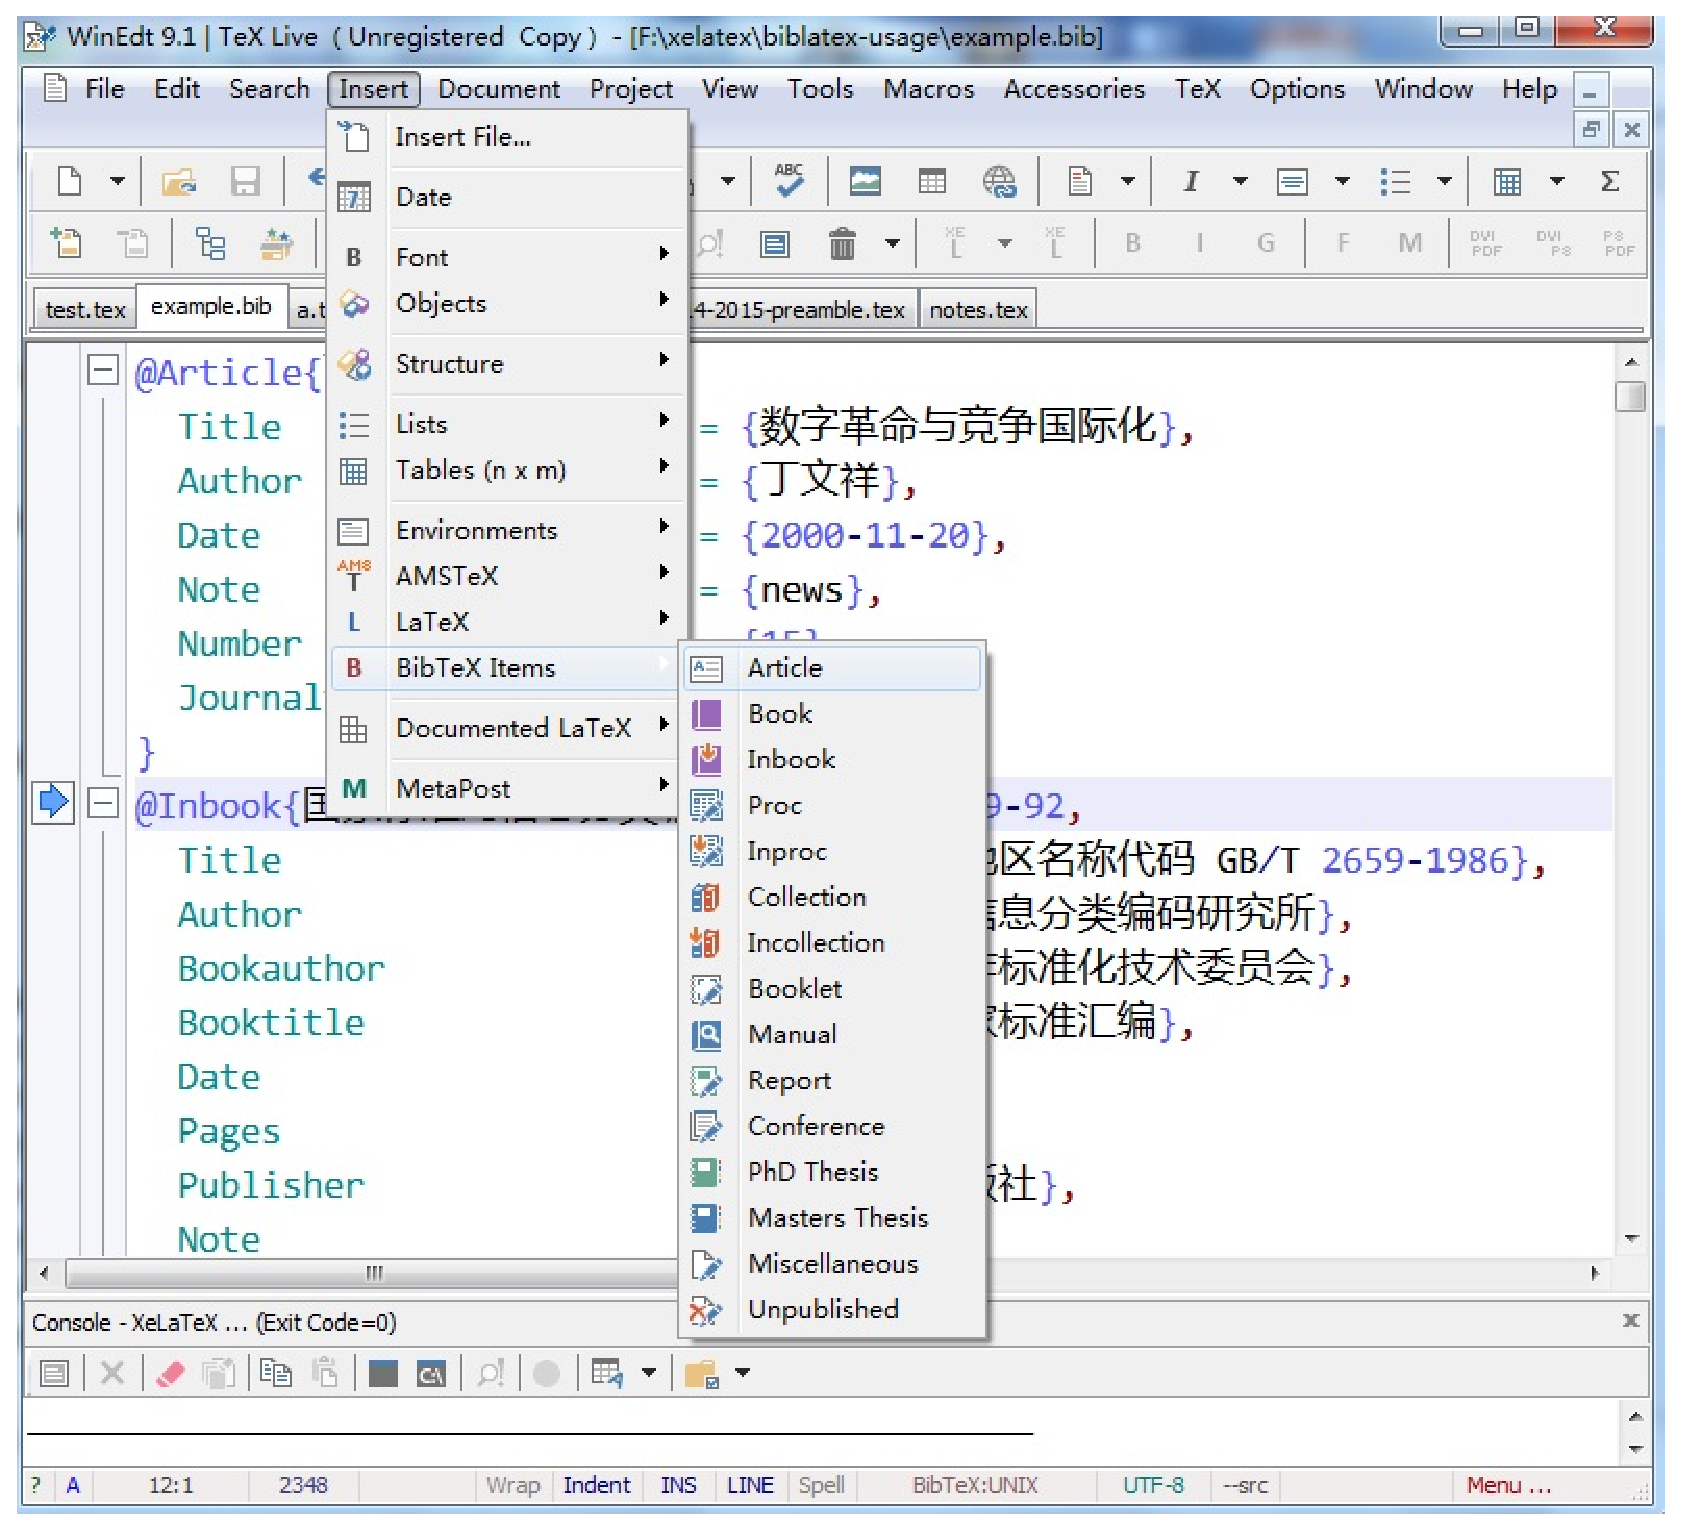
\includegraphics[width=\figwd\textwidth]{bib-winedt}
  \caption{winedt生成bib文件}\label{bib:winedt}
\end{figure}

\subsubsection{利用texstudio生成}
texstudio软件可以在多平台使用,linux下因为没有winedt所以比较常用,用其生成bib文件也很方便,它也提供各种条目类型的信息模板(图\ref{bib:texstudio})。texstudio软件下载地址\url{https://sourceforge.net/projects/texstudio/?source=navbar}。

\begin{figure}[!htb]
  \centering
  \includegraphics[width=\figwd\textwidth]{bib-texstudio}
  \caption{texstudio生成bib文件}\label{bib:texstudio}
\end{figure}

\subsubsection{利用Jabref软件生成}
利用Jabref软件是最重要的一种方式,因为它也是一个较强的参考文献管理工具。新建一个数据库就是新建一个bib文件(图\ref{bib:jabref-a}),新建一个记录就是加入一条参考文献信息(图\ref{bib:jabref-b}),参考文献的信息的录入也是可视化输入栏形式(图\ref{bib:jabref-c})。jabref软件可在官网(\url{http://www.jabref.org/})下载。

\begin{figure}[!htb]
  \centering
  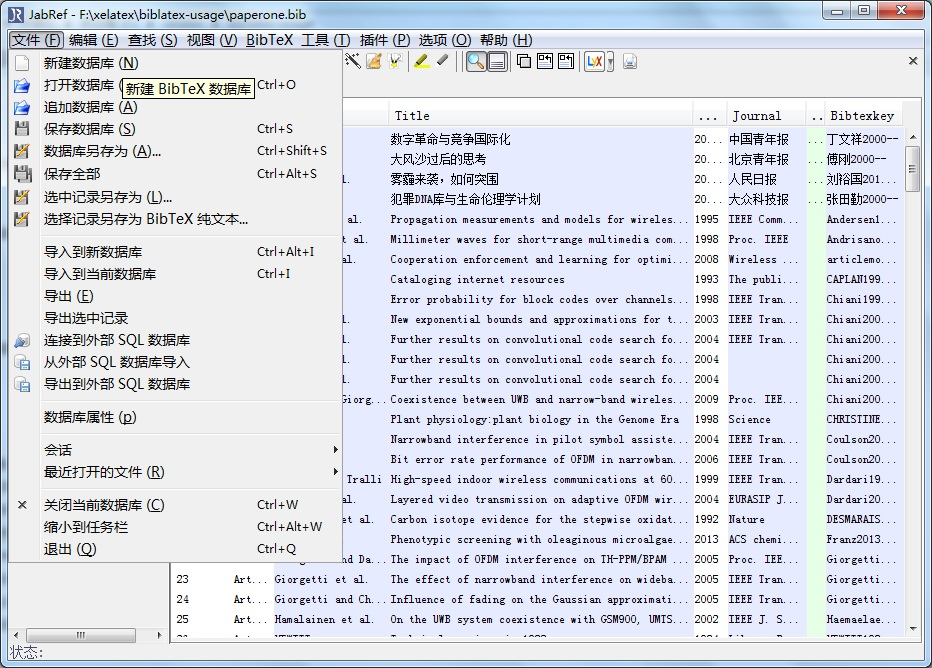
\includegraphics[width=\figwd\textwidth]{bib-jabref-a}
  \caption{Jabref软件生成bib文件}\label{bib:jabref-a}
\end{figure}

\begin{figure}[!htb]
  \centering
  \includegraphics[width=\figwd\textwidth]{bib-jabref-b}
  \caption{Jabref软件增加参考文献条目}\label{bib:jabref-b}
\end{figure}

\begin{figure}[!htb]
  \centering
  \includegraphics[width=\figwd\textwidth]{bib-jabref-c}
  \caption{Jabref软件录入参考文献信息}\label{bib:jabref-c}
\end{figure}

\subsubsection{随\LaTeX 文档生成}
\LaTeX 提供了filecontents环境允许在\LaTeX 文档编译的时候自动将信息写入文件中,自然这也可以用来生成bib文件。比如在导言区加入如下代码,可以生成一个example.bib源文件。
\begin{codetex}{利用filecontents环境随latex文档生成bib}{bib:genwithlatex}
\usepackage{filecontents}
\begin{filecontents}{example.bib}
@Article{傅刚2000--,
  Title                    = {大风沙过后的思考},
  Author                   = {傅刚 and 赵承 and 李佳路},
  Note                     = {news},
  Number                   = {14},
  Url                      = {http://www.bjyouth.com.cn/Bqb/20000412/GB/4216%5ED0412B1401.htm},
  Urldate                  = {2005-07-12},
  Date                     = {2000-04-12},
  Journaltitle             = {北京青年报}
}
@Book{顾炎武1982--,
  Title                    = {昌平山水记},
  Author                   = {顾炎武},
  Publisher                = {北京古籍出版社},
  Year                     = {1982},
  Location                 = {北京},
  Titleaddon               = {东京考古录}
}
\end{filecontents}
\end{codetex}

\subsubsection{获取标准bib文件}
上述给出的方法都是手动编写bib文件的方法,事实上这些手工编写方法还是比较繁琐的。那么是否有其它方法可以直接获取bib文件或其内容避免自己手工编写呢?答案是有的,latexstudio上共分享了这方面的几篇文章\cite{北京交通大学研究生公众号2016--}\cite{olref2016--}\cite{文献助手2016--}。总结起来主要有几个渠道:
\begin{enumerate}
  \item Google 学术: 检索文献 >> Cite(引用) >> BibTeX >> 复制粘贴到 mybibtex.bib 文件
  \item CNKI,(以 firefox 为例): (确保安装 Zotero 的 firefox 扩展 >>) CNKI 检索文献 >> 点击一下 url 输入框末尾的文件夹图标 >> 选中要导出的文献 >> 导出为 BibTeX 引用格式 >> 复制粘贴导出的 BibTeX 文献到 mybibtex.bib 文件。
  \item 必应学术(必应学术 – 学无止境,术有乾坤)、百度学术(百度学术 – 保持学习的态度)类似于google学术。
  \item 从一些学术期刊官网直接获取bib文件,比如IEEE,Springer,Elsevier等
  \item 使用文献助手工具,地址:\url{http://cite.latexstudio.net}
\end{enumerate}

熟练使用这些方法,应该可以进一步提高工作效率。说明一下: latexstudio网站原创、收集、整理了很多latex方面的知识、信息和资源,内容不一,对不同程度的latex爱好者都具有一定的参考价值,各位朋友可以了解学习。


\subsubsection{从pdf或文本文件转换bib文件}
批量生成参考文献数据以构成bib文件,还有一种方式是从参考文献表文本转换。比如从一个包含GB/T 7714-2015格式的参考文献表的pdf文件中,讲文献表拷贝到一个文本文件中,比如 textfilename 文件,其中每一条文献信息构成一个行。然后利用biblatex-gb7714-2015样式宏包附带的perl脚本gb7714texttobib.pl将其转换为bib文件比如bibfilename。该脚本的使用命令为:

\begin{codetex}{利用gb7714texttobib.pl将参考文献文本转换为bib文件}{code:trans2bib}
perl gb7714texttobib.pl in=textfilename out=bibfilename
\end{codetex}

其中in=后面是输入的参考文献文本文件,out=后面是输出的bib文件。

\subsection{\LaTeX 文档的组成}
\LaTeX 文档源文件是由具有某种结构和模式的代码所构成,参考文献自然也遵守这样的结构和模式。

\subsubsection{文档源文件基本结构}
\LaTeX 文档源文件的代码基本结构由导言区和正文区构成,导言区位于documentclass命令与begin\{document\}命令之间,而正文区位于begin\{document\}命令和end\{document\}命令之间。宏包在导言区加载,具体文档内容在正文区编辑。
\begin{codetex}{文档源文件的代码基本结构}{code:doc:structrue}
\documentclass{article}%文档类

%导言区:
%ctex中文设置
\usepackage{ctex}
%定义版面
\usepackage[paperwidth=210mm,paperheight=290mm,left=20mm,right=20mm,top=25mm, bottom=15mm]{geometry}
%书签功能,选项去掉链接红色方框
\usepackage[colorlinks=true,pdfstartview=FitH,linkcolor=blue,anchorcolor=violet,citecolor=magenta]{hyperref}

\begin{document}%正文区开始
正文内容
\end{document}
\end{codetex}

\subsubsection{biblatex宏包、参考文献数据源和样式的加载}
利用 biblatex 宏包生成参考文献可以说非常简单,只要在上述\LaTeX 基本文档基础上载入biblatex宏包和bib数据源,选择需要的参考文献样式,然后在正文需要的地方引用bib文件中准备的参考文献,然后在文档合适位置比如文档末尾打印参考文献表即可,例\ref{code:doc:structrue}和图\ref{fig:eg:ref}给出了示例代码及其结果。

\begin{codetex}{biblatex参考文献生成最小工作示例}{code:doc:structrue}
\documentclass{article}%文档类
%导言区开始:
%加载ctex宏包,中文支持
\usepackage{ctex}
%加载geometry宏包,定义版面
\usepackage[left=20mm,right=20mm,top=25mm, bottom=15mm]{geometry}
%加载hyperref宏包,使用超链接
\usepackage[colorlinks=true,pdfstartview=FitH,linkcolor=blue,anchorcolor=violet,citecolor=magenta]{hyperref}
%加载biblatex宏包,使用参考文献
%其中后端backend使用biber
%标注(引用)样式citestyle,著录样式bibstyle都采用gb7714-2015样式
\usepackage[backend=biber,bibstyle=gb7714-2015,%nature,%
citestyle=gb7714-2015%,backref=true%
]{biblatex}
%biblatex宏包的参考文献数据源加载方式
\addbibresource[location=local]{example.bib}

%正文区开始:
\begin{document}
%正文内容,引用参考文献
详见文献\cite{Peebles2001-100-100}\parencite{Miroslav2004--}
参考文献\cite[见][49页]{蔡敏2006--}\parencite[见][49页]{Miroslav2004--}

%打印参考文献表
\printbibliography[heading=bibliography,title=参考文献]
\end{document}
\end{codetex}

\begin{refsection}
\begin{figure}[!htb]
\centering
\fbox{
\parbox{15cm}{%\raggedright
详见文献\cite{Peebles2001-100-100}\parencite{Miroslav2004--}
参考文献\cite[见][49页]{蔡敏2006--}\parencite[见][49页]{Miroslav2004--}
\printbibliography[heading=subbibliography,title=参考文献]
}
}
\caption{最小工作示例的结果}\label{fig:eg:ref}
\end{figure}
\end{refsection}

其中,biblatex宏包和参考文献数据源都在导言区加载(例\ref{code:pkg:load}),宏包加载命令为usepackage,数据源加载命令为addbibresource。

\begin{codetex}{biblatex宏包、数据源和样式的加载}{code:pkg:load}
%biblatex宏包加载
%其中后端backend使用biber
%引用样式citestyle,著录样式bibstyle都采用gb7714-2015样式
\usepackage[backend=biber,bibstyle=gb7714-2015,%nature,%
citestyle=gb7714-2015%,backref=true%
]{biblatex}

%参考文献数据源加载
\addbibresource[location=local]{example.bib}
\end{codetex}

其中,参考文献样式作为biblatex宏包的可选参数加载,即用bibstyle选项加载著录样式,用citestyle选项加载标注样式,当两者使用同名样式时,可以用一个选项style表示,例\ref{code:pkg:load}中bibstyle和citestyle都选择使用gb7714-2015样式。实际上,标注样式和著录样式分开加载有时是很有用的,有朋友可能想用gb7714-2015的参考文献著录样式,但引用标注又不想要用上标?最简单的方式是著录样式使用gb7714-2015样式,而标注样式使用其他样式比如numeric-comp。当然修改gb7714-2015的标注样式文件中cite等命令也可以实现。参考文献样式还有许多,可以使用biblatex宏包提供的标准样式(标准样式详见biblatex手册Standard Styles一节),或者使用其它作者提供的定制样式,比如nature,science等,具体参见\label{sec:bib:style}节,用户可以根据需要选择使用。

为利用 biblatex 的高级功能,后端 backend 应尽量采用 biber 而不用 bibtex (如果backend为bibtex8,则biblatex宏包利用bibtex8和aux文件进行编译(\LaTeX 传统方法),而backend为biber则是利用biber和bcf文件进行编译)。

另外,biblatex宏包还提供一系列宏包选项,用于控制文献著录表,标注的标签等内容,详细内容参考biblatex手册宏包选项一节。

值得注意的是: 参考文献数据库源文件即bib文件可以是本地的,也可以是网络上的(具体参考biblatex手册Bibliography Commands一节中关于addbibresource命令的说明)。本地的数据源可以指定绝对路径或者相对路径,注意其中目录层级之间的间隔符用/而不是\textbackslash ,windows下默认复制的间隔符是\textbackslash ,需要将其改为/。数据源添加示例见例\ref{ref:addresource}。

\begin{codetex}{添加参考文献数据源的两种方式}{ref:addresource}
\addbibresource{bibfile1.bib} %本地数据源
\addbibresource{bibfile2.bib}
\addbibresource[location=local]{D:/zlatexreference/paperone.bib}
\addbibresource[location=remote]{http://www.citeulike.org/bibtex/group/9517} %网络数据源
\addbibresource[location=remote,label=lan]{ftp://192.168.1.57/~user/file.bib}
\end{codetex}

\subsubsection{文献的标注(引用)}
文献的标注(引用)可以采用\LaTeX 提供的cite命令(注意biblatex对其进行了重定义),也可以使用biblatex提供的其它命令比如parencite等,也可以采用参考文献样式包提供的定制命令比如gb7714-2015样式提供的pagescite,yearpagescite等。在文档中引用文献仅需要在合适的位置插入标注(引用)命令,命令的必选参数是所引用参考文献的bibtex键(引用关键字)。比如:

\begin{codetex}{参考文献的引用命令}{ref:cite:cmd}
详见文献\cite{Peebles2001-100-100}\parencite{Miroslav2004--}
参考文献\cite[见][49页]{蔡敏2006--}\parencite[见][49页]{Miroslav2004--}
详见文献\pagescite{Peebles2001-100-100}\pagescite[][201-301]{Peebles2001-100-100}
见赵耀东\yearpagescite[][205]{赵耀东1998--}和Simon\yearpagescite[][15]{Simon2001--}的文献。
\end{codetex}

当需要在参考文献表中打印不标注的文献时,可以使用nocite命令引入这些文献。其参数是具体条目的引用关键词(bibtex键)或者星号,星号表示将bib文件中所有的参考文献引入。使用命令如:

\begin{codetex}{不标注的文献的引用命令}{ref:nocite:cmd}
参考文献表中打印不标注的文献引入\nocite{Miroslav2004--,蔡敏2006--}。
参考文献表中打印不标注的文献引入,引入bib文件中中全部文献\nocite{*}。
\end{codetex}

另外,在biblatex中使用动态文献集也能产生类似nocite命令的效果,即打印文献表时也会自动输出定义在动态文献集中的文献。

\subsubsection{文献表的打印(输出)}

基于 biblatex 宏包的参考文献表打印(输出)与\LaTeX 传统方式不同,采用的命令是printbibliography。如果全文仅需一个参考文献,那么只要在合适的地方插入如下命令即可:

\begin{codetex}{参考文献表打印命令}{ref:bibprint:cmd}
\printbibliography[heading=bibliography,title=参考文献]
\end{codetex}

注意:printbibliography可以有很多可选参数,用于复杂的文献表控制,具体见biblatex宏包手册。

\subsubsection{参考文献正反超链接}

当加载hyperref宏包后,biblatex宏包除了提供正向超链接外还能提供功能强大的反向超链接。使用方式也很简单,就是使用backref选项。
例\ref{ref:hyperlink:back}给出了代码:
\begin{codetex}{参考文献反向超链接选项}{ref:hyperlink:back}
\usepackage[backend=biber,bibstyle=gb7714-2015,citestyle=gb7714-2015,%
backref=true%
]{biblatex}
\end{codetex}


\subsection{\LaTeX 文档的编译}
文档的编译与\LaTeX 传统方法一致,只是中间的参考文献编译过程略有变化,biblatex宏包使用biber后端时,准备参考文献数据用的命令为biber filename。编译命令可以利用软件调用,也可以自行在命令行输入,下面给出利用winedt、texstudio、命令行、和脚本等不同方式的具体操作过程。

需要注意,无论采用哪种方式编译,如果参考文献数据中存在一些特殊符号比如\&等,编译时会报错。对于这个问题除了手动修改bib文件中参考文献信息这一种方法外,还有两种自动处理方式,一是利用jabref,jabref有bibtex和biblatex两种模式,在biblatex模式下,对于一些特殊字符的输入,比如\&,jabref会自动将其转换为\textbackslash\&。二是使用gb7714-2015样式,在bib数据源不经任何处理的情况下,gb7714-2015样式也能自动处理一些特殊字符。

\subsubsection{利用winedt}
当文档准备好之后,第一步点击winedt工具栏的xelatex按钮(\parbox{1.2cm}{
\includegraphics[width=1.2cm]{button-compiler-winedt}}图中红框内的按钮)完成第一遍\LaTeX 编译;
第二步,打开命令行(可以用winedt菜单accessories下command prompt项)输入命令biber filename完成参考文献数据准备;
第三步,再次点击xelatex编译按钮,完成编译,如果存在反向超链接,那么再次用xelatex编译一遍可以得到正确结果。

\subsubsection{利用texstudio}
texstudio可以多平台使用,在windows和linux下均可。texstudio可以通过利用元命令构建编译命令实现一键编译,进入选项菜单的设置texstudio项,首先在常规选项卡下设置语言为zh\_cn将texstudio界面语言转变为中文,然后在构建选项卡设置默认的编译器为xelatex,设置默认文献工具为biber(图\ref{texstudio:defaulttool}),然后点击构建并查看的配置按钮(\parbox{0.5cm}{
\includegraphics[width=0.5cm]{texstudio-cmd-set}}),设置工具栏构建并查看按钮(\parbox{0.5cm}{
\includegraphics[width=0.5cm]{texstudio-cmd-build}})对应的命令由5个元命令构成(图\ref{texstudio:compilerchain})。这样点击构建并查看按钮即可完成一键编译功能。其编译的过程提示信息如例\ref{texstudio:onekeycompile}所示(环境为windows 7 x64+texlive 2016+tex studio 2.10.8)。

\begin{codetex}{texstudio一键编译过程提示}{texstudio:onekeycompile}
开始 : xelatex.exe -synctex=1 -interaction=nonstopmode "test".tex
完成

开始 : biber.exe "test"
INFO - This is Biber 2.5
INFO - Logfile is 'test.blg'
INFO - Reading 'test.bcf'
INFO - Found 0 citekeys in bib section 0
INFO - Found 4 citekeys in bib section 1
INFO - Found 0 citekeys in bib section 0
INFO - Processing section 1
INFO - Looking for bibtex format file 'example.bib' for section 1
INFO - Decoding LaTeX character macros into UTF-8
INFO - Found BibTeX data source 'example.bib'
WARN - Overwriting field 'year' with year value from field 'date' for entry ' 鍒樻捣娲013--'
WARN - Overwriting field 'year' with year value from field 'date' for entry ' 鑳′紵2011--'
WARN - BibTeX subsystem: C:\Users\ADMINI~1\AppData\Local\Temp\pru9Tr4B7_\example.bib_6592.utf8, line 1198, warning: possible runaway string started at line 1197
INFO - Overriding locale 'en-US' defaults 'normalization = NFD' with 'normalization = prenormalized'
INFO - Overriding locale 'en-US' defaults 'variable = shifted' with 'variable = non-ignorable'
INFO - Sorting list 'none/global/' of type 'entry' with scheme 'none' and locale 'en-US'
INFO - No sort tailoring available for locale 'en-US'
INFO - Writing 'test.bbl' with encoding 'UTF-8'
INFO - Output to test.bbl
INFO - WARNINGS: 3
完成

开始 : xelatex.exe -synctex=1 -interaction=nonstopmode "test".tex
完成

开始 : xelatex.exe -synctex=1 -interaction=nonstopmode "test".tex
完成
\end{codetex}


\begin{figure}[!htb]
  \centering
  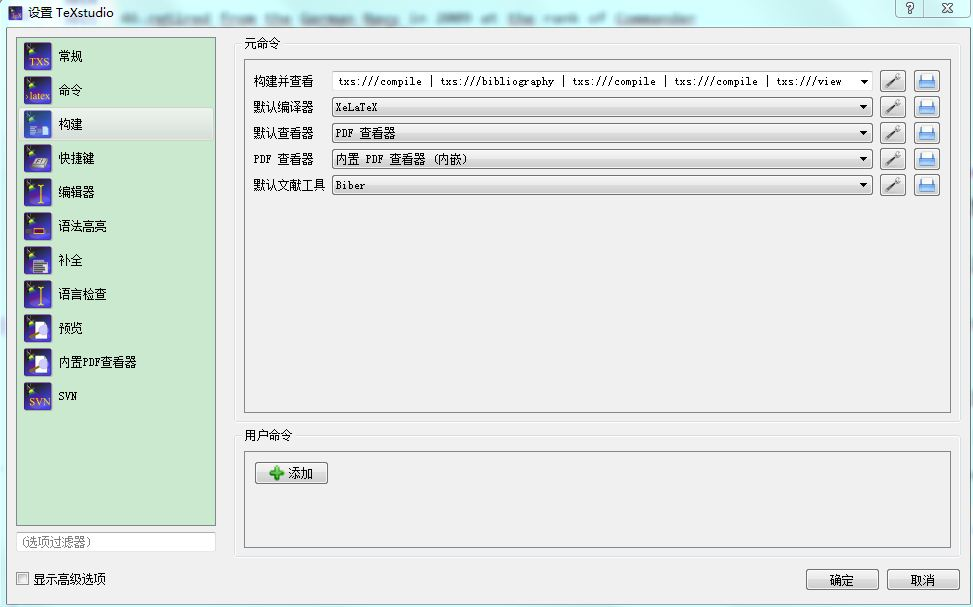
\includegraphics[width=\figwd\textwidth]{texstudio-defaulttool}
  \caption{texstudio设置默认的编译工具}\label{texstudio:defaulttool}
\end{figure}

\begin{figure}[!htb]
  \centering
  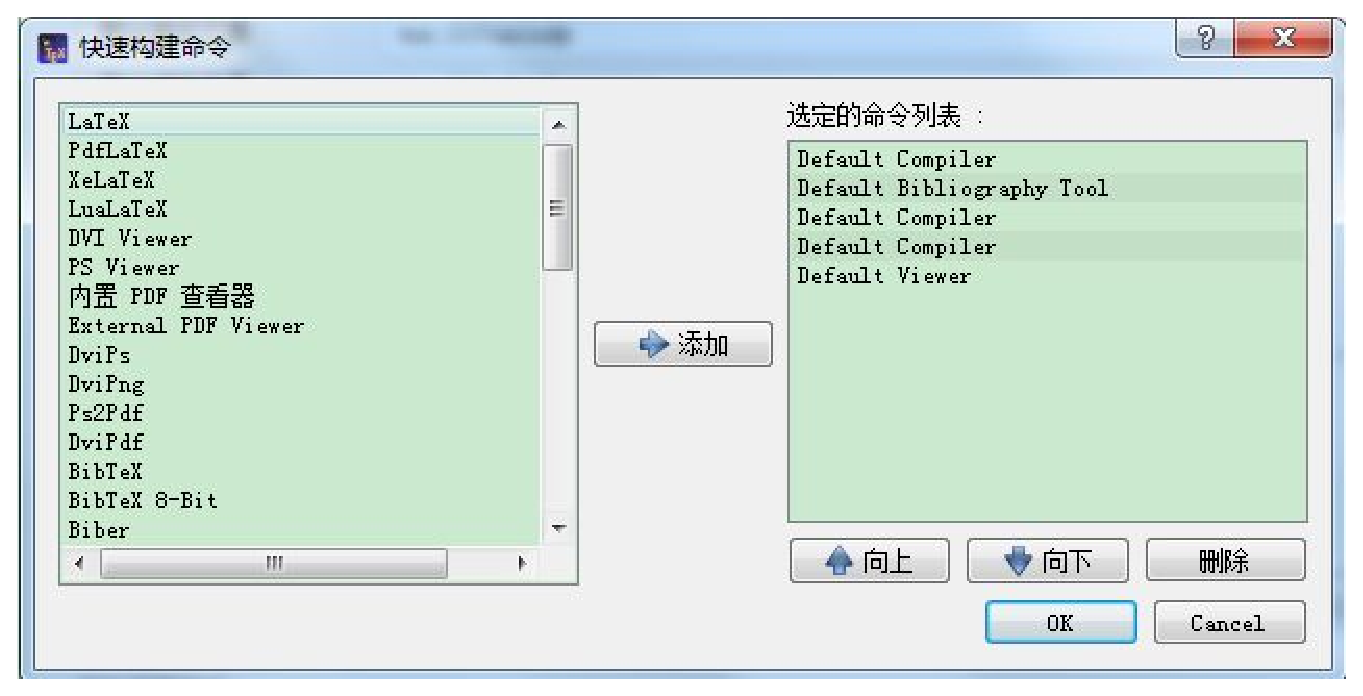
\includegraphics[width=\figwd\textwidth]{texstudio-compilerchain}
  \caption{texstudio配置构建并查看命令}\label{texstudio:compilerchain}
\end{figure}

linux(以deepin linux x64 v15+texlive 2016+texsudio为例)下texstudio的设置是类似的,但要正常编译还有一个关键问题,即还需要设置路径,这不是系统环境的路径设置,而是要告诉texstudio编译工具所在的路径,这同样在菜单选项下的设置texstudio项中设置,仍然进入构建选项卡,左下角点选显示高级选项,然后设置命令(\$PATH)为/usr/local/texlive/2016/bin/x86\_64-linux,如图\ref{texstudio:path:linux}所示。

\begin{figure}[!htb]
  \centering
  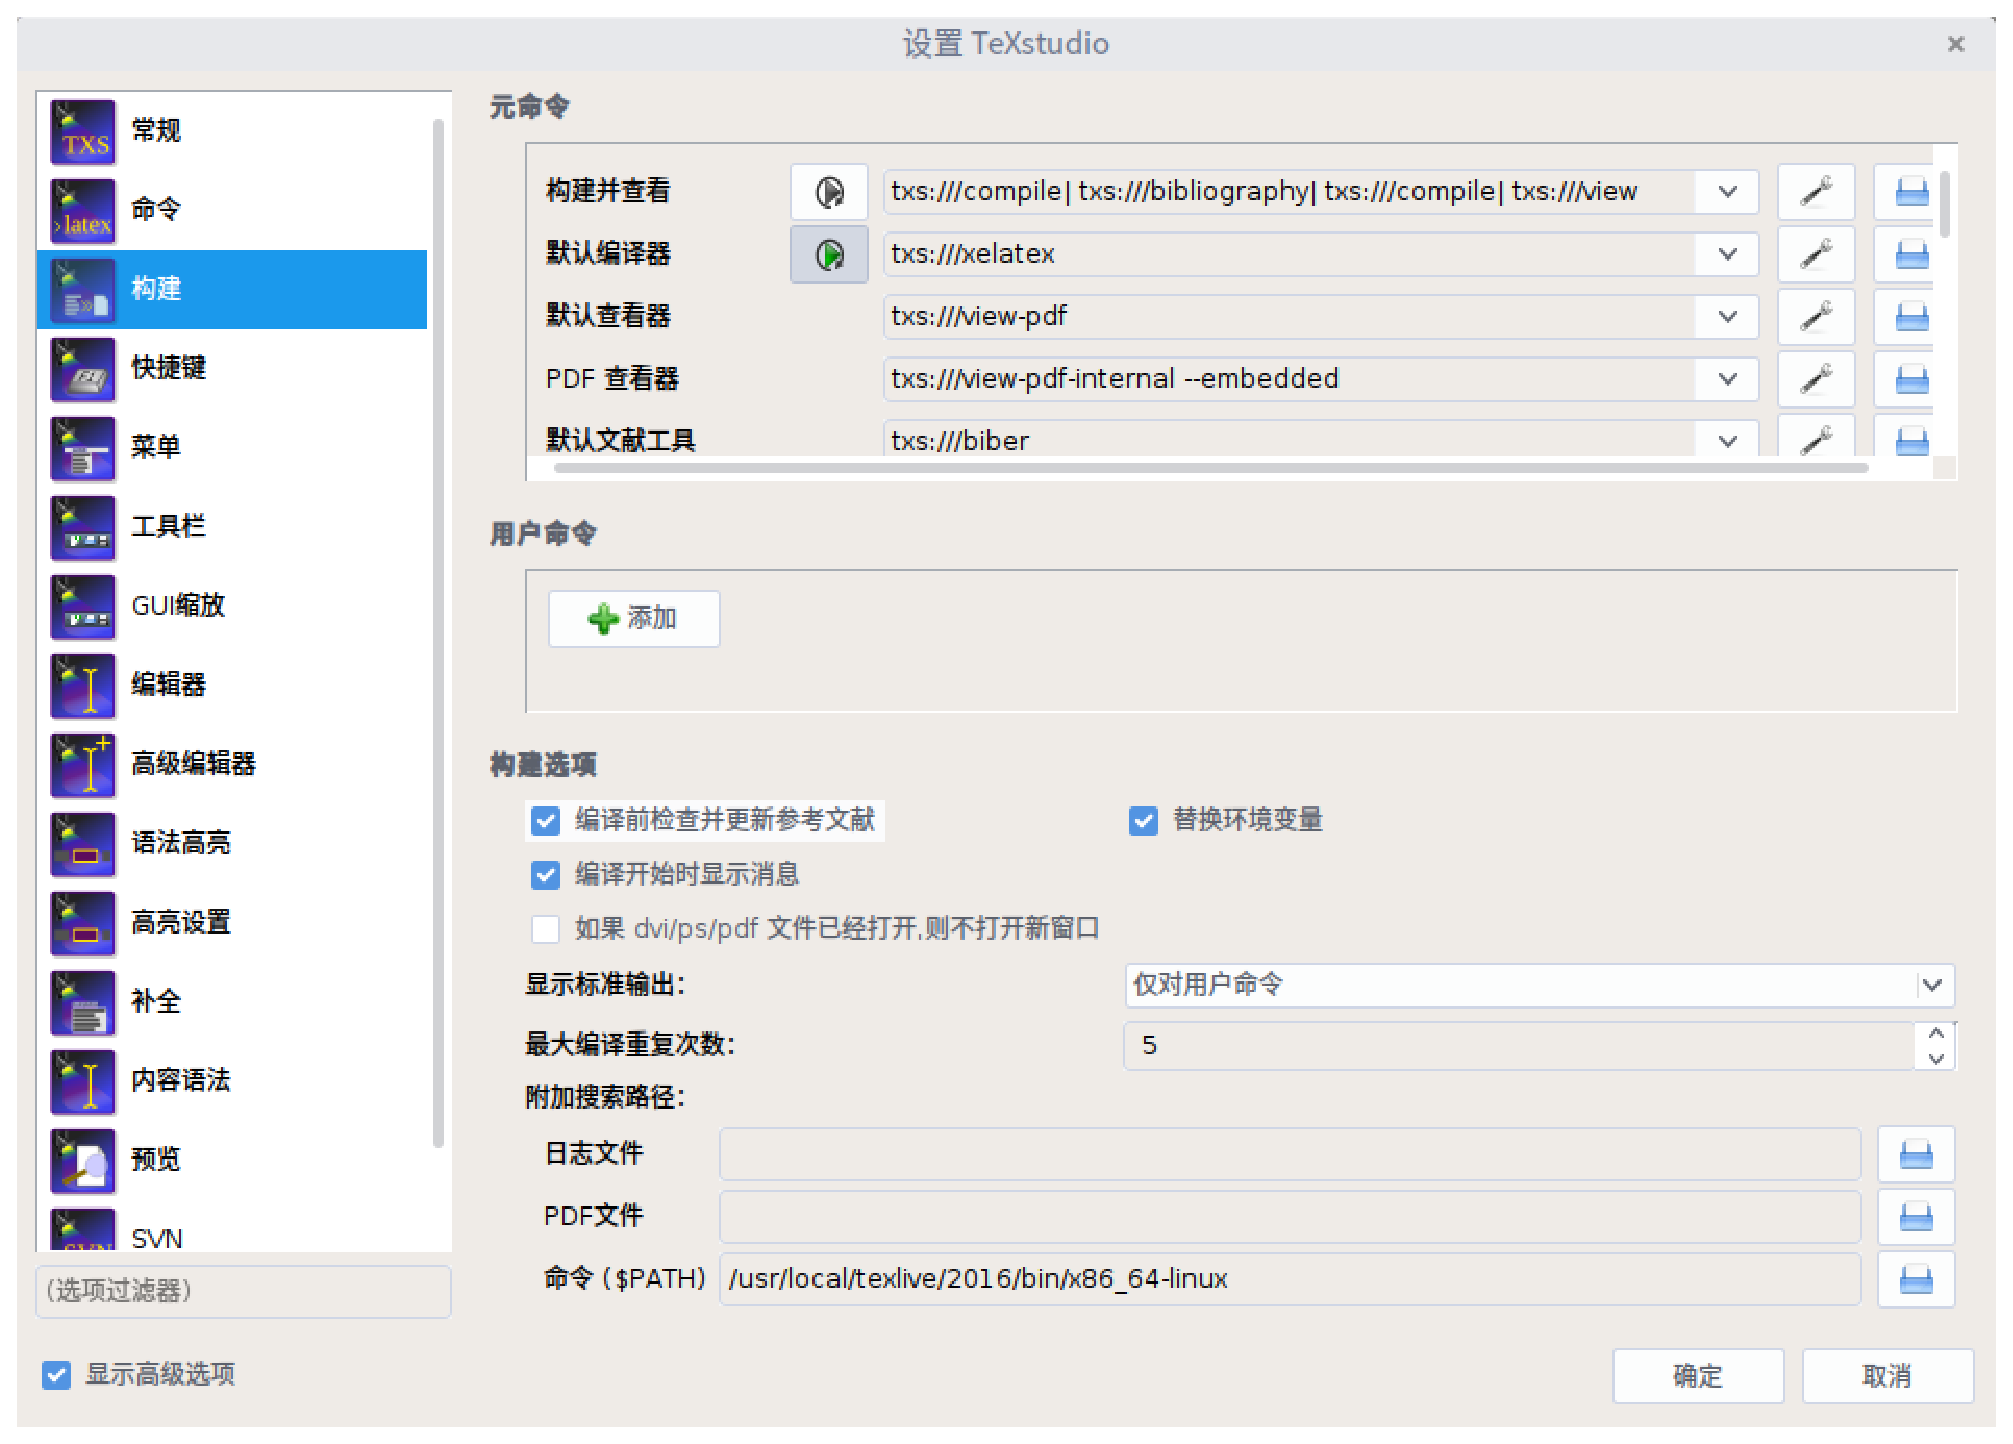
\includegraphics[width=\figwd\textwidth]{texstudio-path-linux}
  \caption{linux下texstudio设置命令路径}\label{texstudio:path:linux}
\end{figure}

\subsubsection{命令行或脚本}

命令行编译本质上是在命令行手动输入命令,命令过程仍然是一遍xelatex编译,biber编译,两边xelatex编译,命令如下:

\begin{codetex}{命令行手动输入的命令}{cmd:prompt}
xelatex.exe -synctex=1 -interaction=nonstopmode "test".tex
biber.exe "test"
xelatex.exe -synctex=1 -interaction=nonstopmode "test".tex
xelatex.exe -synctex=1 -interaction=nonstopmode "test".tex
\end{codetex}


利用脚本编译原理是一样的,只是利用编译脚本文件进行自动编译,注意:linux下的脚本文件需要添加一下路径。比如:
\begin{codetex}{window下的bat脚本文件}{bat:file:cmd}
@echo off
:: compile the tex file
xelatex.exe --synctex=-1 "test".tex
:: compile bibliography
biber "test"
:: compile again
xelatex.exe --synctex=-1 "test".tex
::to do it again for backref
xelatex.exe --synctex=-1 "test".tex
:: clear aux files
del /q *.aux *.bbl *.blg *.log *.out *.toc *.bcf *.xml *.synctex *.nlo *.nls *.bak *.ind *.idx *.ilg *.lof *.lot *.ent-x *.tmp *.ltx *.los *.lol *.loc *.listing *.gz
\end{codetex}

\begin{codetex}{linux下的sh脚本文件}{sh:file:cmd}
#!/bin/bash
# exec path for tex live 2016
export PATH=${PATH}:/usr/local/texlive/2016/bin/x86_64-linux

#compile the tex file
xelatex --synctex=-1 "test".tex
#compile bibliography
biber "test"
#compile again
xelatex --synctex=-1 "test".tex
#to do it again for backref
xelatex --synctex=-1 "test".tex
#clear aux files
rm -r *.aux *.bbl *.blg *.log *.out *.toc *.bcf *.xml *.synctex *.nlo *.nls *.bak *.ind *.idx *.ilg *.lof *.lot *.ent-x *.tmp *.ltx *.los *.lol *.loc *.listing *.gz
\end{codetex}

\subsubsection{利用latexmk宏包}
利用latexmk宏包可以实现一键编译,即使用一条命令即可完成整个编译过程。
\begin{codetex}{latexmk编译命令}{cmd:latexmk}
latexmk -xelatex "test.tex"
\end{codetex}

利用latexmk进行编译的方式也可以在winedt中实现,即定制winedt的工具按钮以实现一键编译功能。具体参见:
\href{https://blog.csdn.net/xenonhu/article/details/80010659}{Winedt 一键编译 LaTeX 文档}

\subsection{分章参考文献和书后参考文献}
分章参考文献在书籍写作中是一种比较常见的需求。在latex传统方法中,利用thebibliography 环境可是实现,但其格式只能在bibitem内输入,对于文献量较大时是不适合的。而利用bibliographystyle 和 bibliography 命令生成的参考文献可以与thebibliography 环境同时存在,生成多个不同的文献表,可以插入多个文献表但却是相同的,这是因为编译文档时,所有的信息都是写入一个 aux 文件中的。所以要实现分章参考文献表,需要使用 chapterbib 或 multibib 宏包,使用chapterbib时要把需要生成文献表的章放到单独的tex文件中,然后用include命令包含进主文件,这样可以生成多个aux文件以便生成分章参考文献表。而使用biblatex宏包可以很方便的在一个\LaTeX 文档中实现多种形式的参考文献划分,其中分章参考文献可以利用refsection环境或者宏包选项来实现。

\subsubsection{利用refsection环境分章}

利用refsection环境可以显式的设置需要打印参考文献的文档结构部分,比如把chapter的所有内容放在refsection环境内,那么在该refsection中使用参考文献打印命令printbibliography就会得到该环境内的参考文献信息,
例\ref{bib:refsection}给出的代码,结果如图\ref{bib:refsection:resa},\ref{bib:refsection:resb}所示。

\begin{codetex}{分章参考文献}{bib:refsection}
\documentclass{report}%%file:egrefsection.tex
\usepackage{ctex}
\usepackage[paperwidth=12cm,paperheight=6cm,top=0cm, bottom=1.5cm, left=1cm,right=1cm]{geometry}
\usepackage{titlesec}
\titleformat{\chapter}{\zihao{4}\heiti}{\thechapter}{1em}{}
\titlespacing*{\chapter}{0pt}{0.0\baselineskip}{0.5\baselineskip}[0pt]
\titleformat{\section}{\zihao{5}\heiti}{\thesection}{1em}{}
\titlespacing*{\section}{0pt}{0.5\baselineskip}{0.5\baselineskip}[0pt]
\usepackage[backend=biber,style=gb7714-2015]{biblatex}
\addbibresource[location=local]{example.bib}

\begin{document}
\chapter{序章}
\begin{refsection}
序章内容\cite{GPS1988--}
\printbibliography[heading=subbibliography,title=本章参考文献]
\end{refsection}

\chapter{正文章一}
\begin{refsection}
正文内容一\cite{杨洪升2013-56-75}
\printbibliography[heading=subbibliography,title=本章参考文献]
\end{refsection}

\chapter{正文章二}
\begin{refsection}
正文内容二\cite{马克思2013-302-302}
\printbibliography[heading=subbibliography,title=本章参考文献]
\end{refsection}
\end{document}
\end{codetex}

\begin{figure}[!htb]
  \centering
  \fbox{
\includegraphics[width=\figwd\textwidth,page=1]{egrefsection.pdf}}
  \caption{分章参考文献举例-序章}\label{bib:refsection:resa}
\end{figure}

\begin{figure}[!htb]
  \centering
  \fbox{
\includegraphics[width=\figwd\textwidth,page=2]{egrefsection.pdf}}
  \caption{分章参考文献举例-章一}\label{bib:refsection:resb}
\end{figure}

\subsubsection{利用宏包refsection选项分章}
除了利用refsection环境显式方法外,还可以利用宏包选项refsection=chapter等来设置需要区分打印参考文献的文档结构,这里设置refsection=chapter表示以章为单位区分打印参考文献,也可以设置成section,那么就是以节为单位进行区分打印。
例\ref{bib:opt:refsection}给出的代码,结果如图\ref{bib:refsection:resc}所示,可以看到其结果与图\ref{bib:refsection:resa}完全一致。

\begin{codetex}{利用宏包选项实现分章参考文献}{bib:opt:refsection}
\documentclass{report}%%file:egrefsectionb.tex
\usepackage{ctex}
\usepackage[paperwidth=12cm,paperheight=6cm,top=0cm, bottom=1.5cm, left=1cm,right=1cm]{geometry}
\usepackage{titlesec}
\titleformat{\chapter}{\zihao{4}\heiti}{\thechapter}{1em}{}
\titlespacing*{\chapter}{0pt}{0.0\baselineskip}{0.5\baselineskip}[0pt]
\titleformat{\section}{\zihao{5}\heiti}{\thesection}{1em}{}
\titlespacing*{\section}{0pt}{0.5\baselineskip}{0.5\baselineskip}[0pt]
\usepackage[backend=biber,refsection=chapter,style=gb7714-2015]{biblatex}
\addbibresource[location=local]{example.bib}

\begin{document}
\chapter{序章}
序章内容\cite{GPS1988--}
\printbibliography[heading=subbibliography,title=本章参考文献]

\chapter{正文章一}
正文内容一\cite{杨洪升2013-56-75}
\printbibliography[heading=subbibliography,title=本章参考文献]

\chapter{正文章二}
正文内容二\cite{马克思2013-302-302}
\printbibliography[heading=subbibliography,title=本章参考文献]
\end{document}
\end{codetex}

\begin{figure}[!htb]
  \centering
  \fbox{
\includegraphics[width=\figwd\textwidth,page=1]{egrefsectionb.pdf}}
  \caption{设置宏包选项实现分章参考文献}\label{bib:refsection:resc}
\end{figure}

\subsubsection{统一的全局参考文献}

biblatex参考文献利用refsection很容易生成分章节的参考文献,但如果要生成一个全局的参考文献,那么可以不使用任何的refsection或者使用一个refsection包含全部的文档(注意:两种方法对于一般情况下都是可以的,但第二种方法对于beamer类则不能使用,这在第\ref{sec:bib:inbeamer}节还会详细说明)。

但还有一种情况是既要生成分章参考文献又要有一个全局的参考文献。那么最简单的方式在文末利用printbibliography的section选项对所有的refsection同时打印一遍,代码如例\ref{bib:global:refsection}所示,但这样的方式更像是文献表堆积,不像一个统一的文献表,且其中的各章的文献引用标注序号不是全局的,只是各refsection内部的序号。

\begin{codetex}{利用refsection的全局参考文献}{bib:global:refsection}
\printbibliography[section=1,heading=subbibliography,title=第一章参考文献]
\printbibliography[section=2,heading=subbibliography,title=第二章参考文献]
\printbibliography[section=3,heading=subbibliography,title=第三章参考文献]
\end{document}
\end{codetex}

这个问题可以用refsegment代替refsection来解决。refsegment与refsection作用很像也用于划分,但其内部的文献序号是全文统一的。每一个segment都有一个编号从1开始,用printbibliography命令打印在某个refsegment环境内的使用参考文献,只需要给出segment=整数的一个值,该值表示第几个refsegment环境。而在refsegment环境外的参考文献默认在segment=0的segment内,若printbibliography命令中给出segment=0则打印不在任一refsegment环境内的文献,若不给出segment参数则遍历所有可以打印的参考文献,包括各个refsegment内的文献。

(注意:refsection内部不可以有refsection,即refsection不可嵌套,但其内部可以使用refsegment。printbibliography命令也可以对refsection内的所有refsegment遍历打印,也可以指定refsection内的某一个refsegment中的文献,只要给出segment参数,当printbibliography在refsection外打印其内refsegment中的文献,则还需指定section参数。

例\ref{eg:global:complex}给出一个测试代码,其结果如图\ref{fig:eg:global:complex}所示。其中“文献全局”命令遍历打印了所有不在refsection内的文献,包括refSegment A,refSegment B,以及不在其内的Gradshteyn文献和附录的Section E中的Parsons文献。

\begin{codetex}{全局参考文献综合示例}{eg:global:complex}
%file:egbibdiv.tex
\documentclass{article}
\usepackage{ctex,hyperref}
\usepackage{geometry}
\geometry{paperwidth=21cm,paperheight=26cm,%
left=1cm,right=1cm,top=1cm,bottom=1.5cm}
\usepackage[backend=biber,style=gb7714-2015]{biblatex}
\addbibresource{example.bib}
\renewcommand{\bibfont}{\zihao{6}}
\usepackage{titlesec}
%\titleformat{command}[shape]{format}{label}{sep}{before}[after]
\titleformat{\section}{\centering\bfseries}{第\thesection 节}{1em}{}[]
\titlespacing*{\section}{0pt}{0.0\baselineskip}{0.0\baselineskip}[0pt]
\titleformat{\subsection}{\flushleft\bfseries}{\S\,\thesubsection}{1em}{}[]
\titlespacing*{\subsection}{0pt}{0.0\baselineskip}{0.0\baselineskip}[0pt]
\begin{document}
\small 	参考文献测试\cite{Gradshteyn2000--}。
	\begin{refsegment}
		\section{refSegment A}
		分章节参考文献测试\cite{Chiani2003-840-845}
		\printbibliography[segment=1,heading=subbibliography,title=文献A]
	\end{refsegment}
	
	\begin{refsegment}
		\section{refSegment B}
		参考文献测试\cite{张敏莉2007-500-503}
	\end{refsegment}
	%\printbibliography放在refsegment环境外也是可以的
	\printbibliography[segment=2,heading=subbibliography,title=文献B]
	
	\begin{refsection}
		\section{refsection C}
		参考文献测试\cite{Zhang2007-500-503}
	\end{refsection}

	\begin{refsection}
		\section{refsection D}
		分章节参考文献测试\cite{Andersen1995-42-49}
    	\begin{refsegment}
			\subsection{refsegment D-1}
			分章节参考文献测试\cite{Simon2004--}。
		\end{refsegment}
		\begin{refsegment}
			\subsection{refsegment D-2}
			分章节参考文献测试\cite{Lin2004--}。
		\end{refsegment}
	\end{refsection}
    \printbibliography[section=2,segment=0,heading=subbibliography,title= 文献D0]
    \printbibliography[section=2,segment=1,heading=subbibliography,title= 文献D1]
    \printbibliography[section=2,segment=2,heading=subbibliography,title= 文献D2]
	\printbibliography[section=1,heading=subbibliography,title=文献C]
    \printbibliography[section=2,heading=subbibliography,title=文献D]
	%遍历非refsection内的参考文献
	\printbibliography[heading=bibliography,title=文献全局]
	\appendix
	\section{Section E}
	参考文献测试\cite{Parsons2000--}。
\end{document}
\end{codetex}

\begin{figure}[!htb]
	\centering
	% Requires \usepackage{graphicx}
	\fbox{
\includegraphics[width=0.9\linewidth]{egbibdiv.pdf}}\\
	\caption{全局参考文献综合示例}\label{fig:eg:global:complex}
\end{figure}

\subsection{筛选、缩略信息、排序、索引}

\subsubsection{文献表分类筛选的不同方法}
除了前述的分章节打印外参考文献可以分类筛选打印,主要基于printbibliography命令的选项来实现。主要包括:
\begin{itemize}
  \item type
  \item nottype
  \item keyword
  \item notkeyword
  \item category
  \item notcategory
  \item filter
  \item check
\end{itemize}
其中category,filter,check是需要手动定义的。

type,nottype分别表示打印是和不是某种条目类型的文献,keyword,notkeyword分别表示打印keywords域中含有或不含有某一个关键词的文献,category,notcategory分别表示是或不是某一设定的category的文献,filter表示属于某一设定筛选器的文献。注意因为category必须要在导言区设置,其实使用并不方便。

\subsubsection{筛选打印示例}

例\ref{eg:bib:filter}给出了这些选项的测试,分别利用type和keyword区分了图书等文献,定义了collections和standard两个筛选器用于打印论文集会议录和标准文献,定义了名为reportandthesis的category用于打印学位论文和报告。结果如图\ref{fig:eg:bibfilter}所示。

\begin{codetex}{分类筛选打印参考文献表}{eg:bib:filter}
%file:egbibfilter
\documentclass{article}
\usepackage{ctex,hyperref}
\usepackage{geometry}
\geometry{paperwidth=21cm,paperheight=26cm,%
left=1cm,right=1cm,top=1cm,bottom=1.5cm}
\usepackage[backend=biber,style=gb7714-2015]{biblatex}
\addbibresource{example.bib}
\renewcommand{\bibfont}{\zihao{6}}
\usepackage{titlesec}
%\titleformat{command}[shape]{format}{label}{sep}{before}[after]
\titleformat{\section}{\centering\bfseries}{第\thesection 节}{1em}{}[]
\titlespacing*{\section}{0pt}{0.0\baselineskip}{0.0\baselineskip}[0pt]
\titleformat{\subsection}{\flushleft\bfseries}{\S\,\thesubsection}{1em}{}[]
\titlespacing*{\subsection}{0pt}{0.0\baselineskip}{0.0\baselineskip}[0pt]
\DeclareBibliographyCategory{reportandthesis}
\addtocategory{reportandthesis}{汤万金2013-09-30--,Calkin2011-8-9,吴云芳2003--,CALMS1965--}
\begin{document}
文献\cite{张伯伟2002--}\cite{CRAWFPRD1995--}\cite{陈志勇2011--}\cite{Babu2014--}\cite{汤万金2013-09-30--}
\cite{Calkin2011-8-9}\cite{吴云芳2003--}\cite{CALMS1965--}\cite{张凯军2012-04-05--}\cite{KOSEKI2002--}
\cite{全国广播电视标准化技术委员会2007-1-1}\cite{国家环境保护局科技标准司1996-2-3}
\cite{楼梦麟2011-11-12}\cite{BUSECK1980-117-211}\cite{陈建军2010-93-93}
\cite{DESMARAIS1992-605-609}\cite{张田勤2000--}\cite{萧钰2001--}

\printbibliography[type=book,notkeyword=standard,title=【普通图书】]
\defbibfilter{collections}{%
type=collection
or type=proceedings
or type=incollection
or type=inproceedings
}
\printbibliography[filter=collections,title=【论文集、会议录】]
\defbibfilter{standard}{%
( type=book or type=inbook )
and keyword=standard
}
\printbibliography[filter=standard,title=【标准文献】]
\printbibliography[type=inbook,notkeyword=standard,title=【专著中析出的文献】]
\printbibliography[type=article,notkeyword=news,title=【期刊中析出的文献】]
\printbibliography[type=article,keyword=news,title=【报纸析出的文献】]
\printbibliography[category=reportandthesis,title=【报告和学位论文】]
\printbibliography[notcategory=reportandthesis,title=【非报告和学位论文】]
\end{document}
\end{codetex}

\begin{figure}[!htb]
  \centering
  \fbox{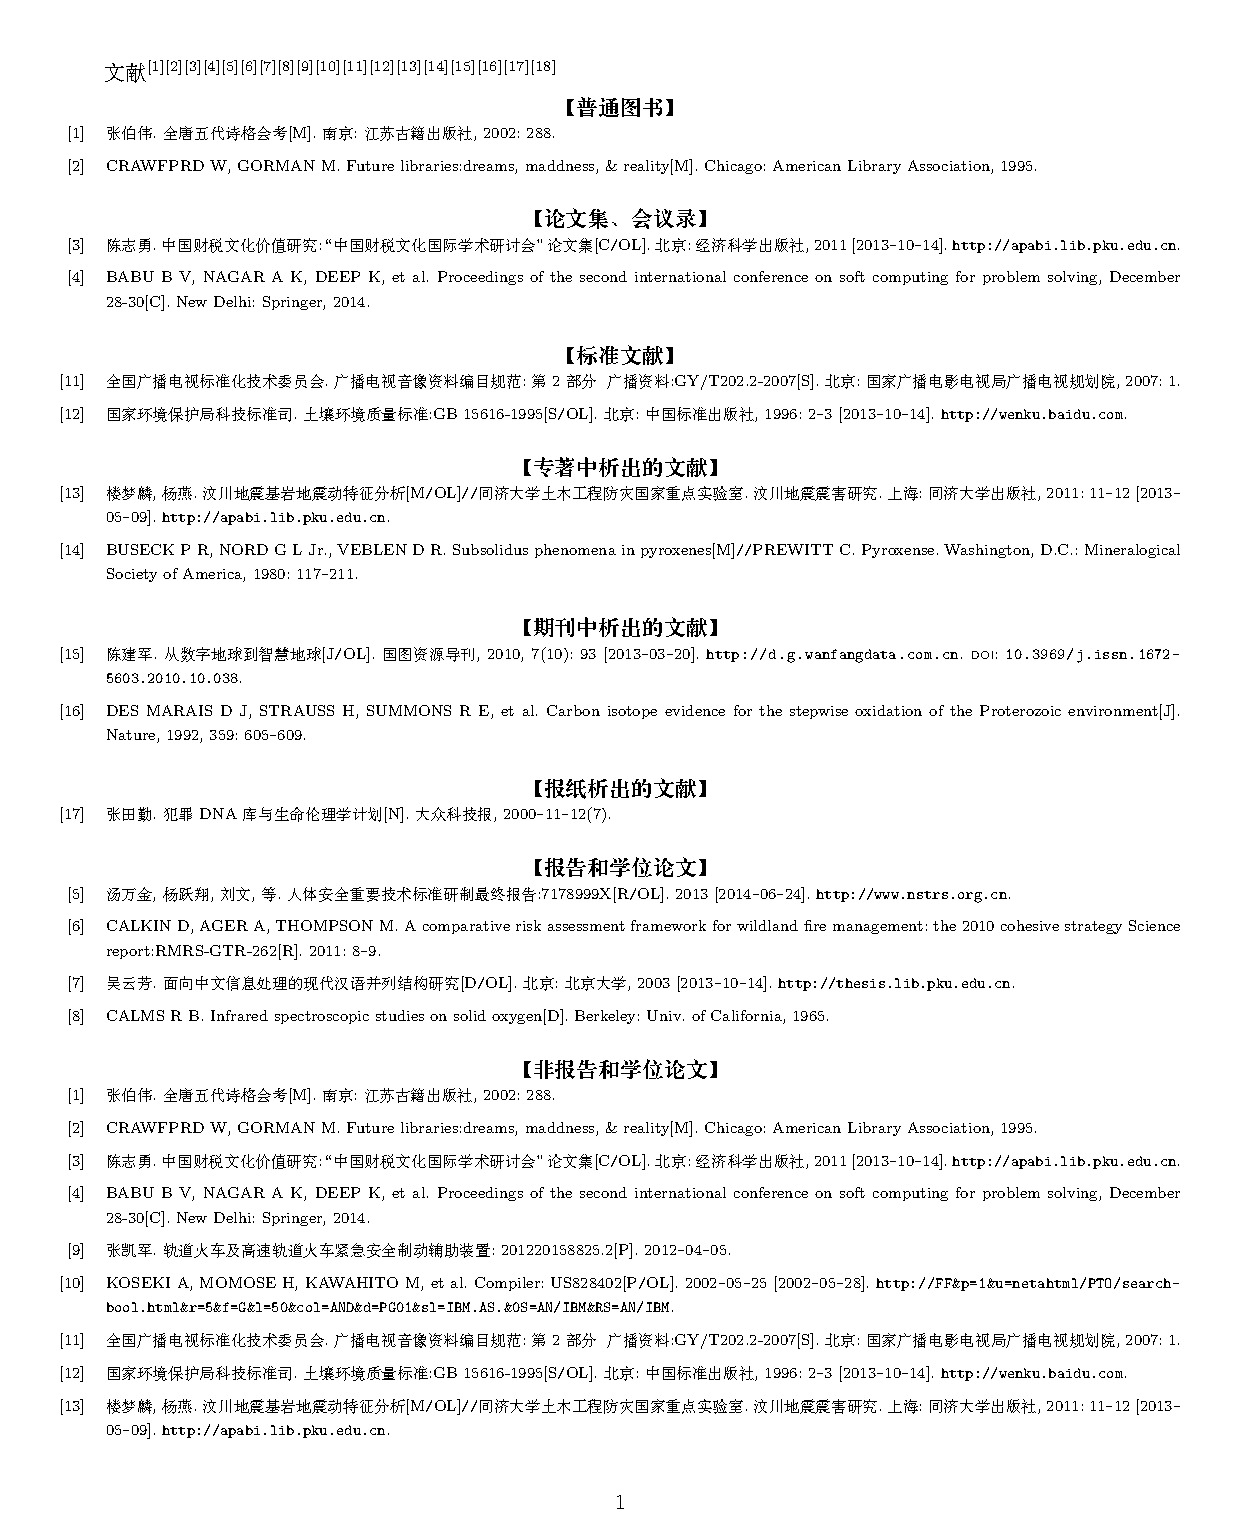
\includegraphics[width=0.8\textwidth,page=1]{egbibfilter.pdf}}
  \caption{脚注和旁注中参考文献表}\label{fig:eg:bibfilter}
\end{figure}


\subsubsection{文献缩略信息打印}

缩略信息打印示例,如例\ref{eg:print:biblist}所示。

\begin{codetex}{论文集信息打印}{eg:print:biblist}
\documentclass[twoside]{article}
\usepackage{ctex}
\usepackage{geometry}
\geometry{paperwidth=21cm,paperheight=29cm,top=1.5cm, bottom=1.5cm, left=2.54cm,right=2.54cm}
\usepackage{xcolor}
\usepackage[CJKbookmarks,colorlinks,bookmarksnumbered=true,pdfstartview=FitH,linkcolor=blue]{hyperref}
%\usepackage[backend=biber,style=gb7714-2015,maxbibnames=5,minbibnames=5]{biblatex}
\usepackage[backend=biber,style=gb7714-2015,gbpunctin=false]{biblatex}%align=gb7714-2015

\DefineBibliographyStrings{english}{in={}}

\DeclareBibliographyDriver{shortbooktitle}{%
\printfield{booktitle}\par}

\defbibcheck{shortbooktitle}{%
\iffieldundef{booktitle}{\skipentry}
{\ifcsdef{\strfield{shortbooktitle}=\strfield{booktitle}}{\skipentry}
{\savefieldcs{booktitle}{\strfield{shortbooktitle}=\strfield{booktitle}}}}%
}
%注意这里savefieldcs给命令拷贝booktitle域的信息是无关紧要的,
%如果有其他定义命令的序列比如savecs{\strfield{shortbooktitle}=\strfield{booktitle}}也是一样的,
%因为前面的ifcsdef判断只是判断命令是否存在,但因为biblatex中提供了savefieldcs命令所以应用它


\usepackage{filecontents}
\begin{filecontents}{\jobname.bib}
@Inproceedings{refa,
  Title                    = {Interference cartography for hierarchical dynamic spectrum access},
  Address                  = {Chicago, IL},
  Author                   = {AlayaFeki, A. and B. Sayrac and S. Ben Jemaa and E. Moulines},
  editor={Name, B and Dome, C},
  Booktitle                = {Proc. IEEE Symp. on New Frontiers in Dynamic Spectrum Access Networks (DySPAN)},
  Date                     = {2008-10},
  Pages                    = {1-5}
}

@Inproceedings{refb,
  Title                    = {Interference cartography for hierarchical dynamic spectrum access},
  Address                  = {Chicago, IL},
  editor={Name, B and Dome, C},
  Author                   = {BlayaFeki, A. and B. Sayrac and S. Ben Jemaa and E. Moulines},
  Booktitle                = {Proc. IEEE Symp. on New Frontiers in Dynamic Spectrum Access Networks (DySPAN)},
  Date                     = {2008-10},
  Pages                    = {1-5}
}

@Inproceedings{refc,
  Title                    = {Interference cartography for hierarchical dynamic spectrum access},
  Address                  = {Chicago, IL},
  bookauthor={Name, B and Dome, C},
  Author                   = {ClayaFeki, A. and B. Sayrac and S. Ben Jemaa and E. Moulines},
  Booktitle                = {Proc. IEEE Symp. on New Frontiers in Dynamic Spectrum Access Networks (DySPAN)},
  Date                     = {2008-10},
  Pages                    = {1-5}
}

@Inproceedings{refd,
  Title                    = {Interference cartography for hierarchical dynamic spectrum access},
  Address                  = {Chicago, IL},
  bookauthor={Name, B and Dome, C},
  Author                   = {MlayaFeki, A. and B. Sayrac and S. Ben Jemaa and E. Moulines},
  Booktitle                = {Proc. IEEE Symp. on New Frontiers in Dynamic Spectrum Access Networks (DySPAN)},
  Date                     = {2008-10},
  Pages                    = {1-5}
}

@Inproceedings{FOURNEY1971-17-38,
  Title                    = {Advances in holographic photoelasticity},
  Author                   = {M E FOURNEY},
  Booktitle                = {Symposium on Applications of Holography in Mechanics, August 23-25, 1971, University of Southern California, Los Angeles, California},
  Date                     = {1971},
  Pages                    = {17-38},
  Publisher                = {ASME},
  Location                 = {New York}
}

@Inproceedings{裴丽生1981-2-10,
  Title                    = {在中国科协技术期刊编辑工作经验交流会上的讲话},
  Author                   = {裴丽生},
  Booktitle                = {中国科协学术期刊编辑工作经验交流会资料选},
  Date                     = {1981},
  Pages                    = {2-10},
  Institution              = {中国科学技术协会学会工作部},
  Location                 = {北京}
}

@Book{Simon2001--,
  Title                    = {Spread Spectrum Communications Handbook},
  Address                  = {New York City},
  Author                   = {Simon, M. K. and Omura,J. K. and Scholtz,R. A. and Levitt,B. K.},
  Publisher                = {McGraw-Hill, Inc.},
  Year                     = {2001}
}
\end{filecontents}
\addbibresource{\jobname.bib}


\begin{document}
编译信息:biblatex v\versionofbiblatex;gb7714-2015*.* version number \versionofgbtstyle.

\section{文献表}
文献
\cite{refc}
\cite{refa}
\cite{refb}
\cite{refd}
\cite{FOURNEY1971-17-38}
\cite{裴丽生1981-2-10}
\cite{Simon2001--}

\printbiblist[title={book Shorthands}]{shortbooktitle}

\printbibliography%[heading=subbibintoc,title=【参考文献】]
\end{document}
\end{codetex}

\subsubsection{文献表和标注的排序}

排序涉及到两个方面的内容,一是文献表中的排序,二是标注的排序。其中标注的排序通常是在同一位置标注多个标签时,这种情况往往是多个引用关键字(词)传递给一个标注(引用)命令。一般情况下标注是不进行排序的,而是以引用时给出的顺序进行排序,当需要进行标签排序时需要启用sortcites选项,这时biblatex会按照当前文献表中的顺序对标注标签进行排序。

而文献表中的文献排序由sorting选项控制,常见的值包括:

\begin{description}
\item[nty] %Sort by name, title, year.
按照姓名、标题、年份排序。
\item[nyt] %Sort by name, year, title.
按照姓名、年份、标题排序。
\item[nyvt] %Sort by name, year, volume, title.
按照姓名、年份、卷数、标题排序。
\item[anyt] %Sort by alphabetic label, name, year, title.
按照字母标签、姓名、年份、标题排序。
\item[anyvt] %Sort by alphabetic label, name, year, volume, title.
按照字母标签、姓名、年份、卷数、标题排序。
\item[ynt] %Sort by year, name, title.
按照年份、姓名、标题排序。
\item[ydnt] %Sort by year (descending), name, title.
按照年份(降序)、姓名、标题排序。
\item[none] %Do not sort at all. All entries are processed in citation order.
不进行排序。所有的条目按照引用顺序处理。
\item[debug] %Sort by entry key. This is intended for debugging only.
按照条目键值排列。该选项只用于程序调试。
\item[name] %Use \prm{name}, as defined with \cmd{DeclareSortingTemplate} (\secref{aut:ctm:srt})
使用由 \verb|DeclareSortingTemplate|定义的排序模板名 name。
\end{description}
注意:除非另加说明,文献条目总是按升序排列。

通常情况下,在选择使用某种样式时,文献表的排序方式就已经设定。当需要调整排序时,就需要在加载biblatex宏包时显式地给出sorting选项,并可根据需要选择上述给出的选项值。

另外,因为biber能充分利用perl的一些模块的功能,所以biblatex还能根据Unicode::Collation::locale模块提供不同语言的排序的本地化调整方案。对于中文,默认的排序规则是按照中文字符的unicode编码进行排序,但可以通过设置选项来进行调整,对于中文有如下调整方案:zh,zh\_\_pinyin,zh\_\_big5han,zh\_\_gb2312han,zh\_\_stroke,zh\_\_zhuyin。

一般的,biblatex利用sortlocale选项将调整方案名传递给biber,biber利用 Unicode::Collation::locale 模块提供对应的排序。因此biblatex可以设置选项为:
  \begin{itemize}
    \item \verb|sortlocale=auto| 或者不设置该选项,为默认的unicode编码顺序
    \item \verb|sortlocale=zh|,为unicode编码顺序
    \item \verb|sortlocale=zh__pinyin|,为拼音顺序
    \item \verb|sortlocale=zh__big5han|,为big5 编码顺序
    \item \verb|sortlocale=zh__gb2312han|,为GB-2312 顺序
    \item \verb|sortlocale=zh__stroke|,为笔划数顺序
    \item \verb|sortlocale=zh__zhuyin|,为注音顺序
  \end{itemize}
中文排序本地化调整的测试文档见
\href{run:exampleandimage/testlocale.tex}{testlocale.tex}

当然这种调整可以直接利用在biber编译时设置相应的选项来实现,比如需要按拼音或字顺进行排序时,可使用biber选项,此时biblatex不需要设置sortlocale选项。

\begin{codetex}{中文文献排序时的biber选项}{eg:sort:bibercmd}
%按拼音排序,biber命令
biber -l zh__pinyin jobname
%按笔画排序,biber命令
biber -l zh__stroke jobname
\end{codetex}

一个简单的中文作者排序示例见\href{https://github.com/hushidong/biblatex-gb7714-2015/wiki}{(八)如何对文献表中的参考文献进行排序?}

有的时候,可能希望标注标签的排序和文献表中的顺序不同,操作方法,可以参考
\href{https://github.com/hushidong/biblatex-gb7714-2015/issues/30}{citation的顺序和bibliography的顺序如何不关联}。其中使用了biblatex宏包提供参考文献文境的概念,即不同的文境下可以使用不同的排序方式。


\subsubsection{文献信息索引}

当需要对参考文献的信息进行索引时,可以使用indexing选项。启用indexing后,biblatex的标准样式默认会将作者和题名加入到索引中去,如果需要增加一些信息的索引则需要对样式文件做修改。另外,要生成索引还需要使用索引相关的宏包,如makeidx。宏包加载如例\ref{eg:print:index}所示:

\begin{codetex}{文献信息索引}{eg:print:index}
\documentclass[twoside]{article}
\usepackage{ctex}
\usepackage{geometry}
\geometry{paperwidth=21cm,paperheight=29cm,top=1.5cm, bottom=1.5cm, left=2.54cm,right=2.54cm}
\usepackage{xcolor}
\usepackage[CJKbookmarks,colorlinks,bookmarksnumbered=true,pdfstartview=FitH,linkcolor=blue]{hyperref}
\usepackage[backend=biber,style=gb7714-2015,gbtype=true,block=none,indexing=true]{biblatex}%align=gb7714-2015
\addbibresource[location=local]{example.bib}
\usepackage{makeidx}
\makeindex

\begin{document}

\section{文献表}
文献
\cite{张伯伟2002--}
\cite{白书农1998-146-163}
\cite{杨洪升2013-56-75}
\cite{中华医学会湖北分会1984--}
\cite{雷光春2012--}
\cite{贾东琴2011-45-52}
\cite{汤万金2013-09-30--}
\cite{韩吉人1985-90-99}
\cite{马欢2011-27-27}
\cite{张凯军2012-04-05--}
\cite{国家环境保护局科技标准司1996-2-3}
\cite{中国职工教育研究会1985--}
\cite{丁文祥2000--}
\cite{李强2012-05-03--}

\cite{OBRIEN1994--}
\cite{FOURNEY1971-17-38}
\cite{Park2010-696-715}
\cite{Babu2014--}
\cite{Calkin2011-8-9}
\cite{CALMS1965--}
\cite{KOSEKI2002--}
\cite{standardinfoiso158}
\cite{Dublin2012-06-14--}

\printbibliography
\printindex
\end{document}
\end{codetex}

\subsection{参考文献标题格式}

期刊文章经常需要设置某种格式的参考文献标题,包括字号,大小,段落格式等。在书籍等写作中有时还需要将参考文献加入目录中,以便实现超链接。
\subsubsection{加入目录链接}

加入目录的命令是addcontentsline,在printbibliography命令前使用该命令即可将参考文献加入目录中,同时为了能够超链接正确可以加入hyperref宏包提供的phantomsection命令。例\ref{bib:inserttoc}给出了代码。
\begin{codetex}{手动加入目录链接}{bib:inserttoc}
\addcontentsline{toc}{chapter}{参考文献}
\phantomsection
\printbibliography[heading=bibliography,title=本章参考文献]
\end{codetex}

除了上述手动添加的方式外,还可以在printbibliography命令使用biblatex提供的选项来实现,比如heading=bibintoc,该选项与heading=bibliography是类似的,只是增加了在目录中加入链接的功能,例\ref{bib:inserttoc:bibintoc}给出了代码。
\begin{codetex}{使用bibintoc加入目录链接}{bib:inserttoc:bibintoc}
\printbibliography[heading=bibintoc,title=本章参考文献]
\end{codetex}

\subsubsection{重定义heading}

默认情况下,biblatex参考文献标题的格式主要依赖于\LaTeX 文档的章节的标题格式。当printbibliography中使用heading选项的参数是bibliography和bibintoc时,参考文献标题的格式与当前文档类的主划分单元的标题格式一致,比如book和report类中与chapter一致,而在article类中与section一致。heading选项的参数是subbibliography和subbibintoc时,则与主单元的下一层级的标题格式一致,即book和report类中与section一致,而在article类中与subsection一致。因此设置参考文献标题的格式最简单方式是设置文档的各级标题格式然后选择heading选项的参数(注意当heading选项不给出时,其默认参数为bibliography)。

事实上利用defbibheading命令重定义bibliography等heading的相关信息可以改变默认的标题对应方式,比如可以将bibliography与subsubsection层级标题格式对应起来,例\ref{bib:def:headsec}给出了代码。其中还使用了phantomsection和addcontentsline命令可以完成上一小节需要的加入目录链接功能。其中还使用了centering使标题居中,这预示了一种标题格式修改方式,甚至可以不使用文档类的标题格式而直接自定义标题。

\begin{codetex}{biblatex对于目录的影响}{bib:def:headsec}
\usepackage[backend=biber,style=gb7714-2015ay]{biblatex}
\defbibheading{bibliography}[\bibname]{%
\phantomsection%解决链接指引出错的问题,相当于加入了一个引导点
\addcontentsline{toc}{subsubsection}{#1}
	\centering\subsubsection*{#1}}%
\end{codetex}

需要注意,如果要使用titleps作为页眉页脚的设置宏包,那么需要利用defbibheading重设一下heading选项参数,因为默认情况下heading的参数比如bibliography中带有markboth命令,该命令与titleps共用时会导致页眉页脚一些出现问题。例\ref{bib:def:heading}给出了代码。而使用文档类默认的页眉页脚或者利用fancyhdr设置页眉页脚,则不需要修改。为了方便移植应用,这里给出三种设置页眉页脚的代码,例\ref{head:class:ctex}是使用文档类提供和ctex修改的页眉页脚;例\ref{head:fancyhdr}是使用fancyhdr设置的页眉页脚;例\ref{head:titleps}是使用titleps设置的页眉页脚。

\begin{codetex}{重设heading选项参数}{bib:def:heading}
\defbibheading{bibliography}[\bibname]{%
	\chapter*{#1}}%
%	\markboth{#1}{#1}}
%重定义命令中去掉了markboth那一句命令。
\end{codetex}

\begin{codetex}{文档类提供ctex修改的页眉页脚举例}{head:class:ctex}
%file:egheadclass.tex
\documentclass{book}
\usepackage{ctex}
\usepackage[paperwidth=12cm,paperheight=6cm,top=1.5cm, bottom=1.5cm, left=1cm,right=1cm]{geometry}
\usepackage{titlesec}
\titleformat{\chapter}{\zihao{4}\heiti}{\thechapter}{1em}{}
\titlespacing*{\chapter}{0pt}{0.0\baselineskip}{0.5\baselineskip}[0pt]
\titleformat{\section}{\zihao{5}\heiti}{\thesection}{1em}{}
\titlespacing*{\section}{0pt}{0.5\baselineskip}{0.5\baselineskip}[0pt]
\usepackage[backend=biber,style=nature]{biblatex}
\addbibresource[location=local]{example.bib}

\renewcommand{\bibfont}{\zihao{-6}\songti}
\setlength{\bibitemsep}{2pt}
\usepackage{hyperref}
\begin{document}
\tableofcontents
\begin{refsection}
\chapter{序章}
\section{序节}
序章内容\cite{GPS1988--}
\defbibentryset{bilangyi2013}{易仕和2013--,Yi2013--}
专著,双语文献引用\cite{bilangyi2013}

\phantomsection
\addcontentsline{toc}{chapter}{参考文献}
\printbibliography[heading=bibliography,title=本章参考文献]
\end{refsection}

\begin{refsection}
\chapter{正文章一}
\section{正文节一}
正文内容一\cite{杨洪升2013-56-75}

\phantomsection
\addcontentsline{toc}{section}{参考文献}
\printbibliography[heading=subbibliography,title=本章参考文献]
\end{refsection}

\begin{refsection}
\chapter{正文章二}
\section{正文节二}

正文内容二\cite{马克思2013-302-302}
\printbibliography[heading=subbibliography,title=本章参考文献]
\end{refsection}
\end{document}
\end{codetex}

\begin{codetex}{利用fancyhdr生成页眉页脚举例}{head:fancyhdr}
%file:egheadfancy.tex
\documentclass{book}
\usepackage{ctex}
\usepackage[paperwidth=12cm,paperheight=6cm,top=1.5cm, bottom=1.5cm, left=1cm,right=1cm]{geometry}
\usepackage{titlesec}
\titleformat{\chapter}{\zihao{4}\heiti}{\thechapter}{1em}{}
\titlespacing*{\chapter}{0pt}{0.0\baselineskip}{0.5\baselineskip}[0pt]
\titleformat{\section}{\zihao{5}\heiti}{\thesection}{1em}{}
\titlespacing*{\section}{0pt}{0.5\baselineskip}{0.5\baselineskip}[0pt]
\usepackage[backend=biber,style=nature]{biblatex}
\addbibresource[location=local]{example.bib}

\renewcommand{\bibfont}{\zihao{-6}\songti}
\setlength{\bibitemsep}{2pt}
\usepackage{hyperref}
\usepackage{fancyhdr}
\pagestyle{fancy}
\renewcommand{\chaptermark}[1]{%
\markboth{#1}{}}
\renewcommand{\sectionmark}[1]{%
\markright{\thesection\ #1}}
\fancyhf{} % delete current header and footer
\fancyhead[LE,RO]{\bfseries\thepage}
\fancyhead[LO]{\bfseries\rightmark}
\fancyhead[RE]{\bfseries\leftmark}
\renewcommand{\headrulewidth}{0.5pt}
\renewcommand{\footrulewidth}{0pt}
\addtolength{\headheight}{0.5pt} % space for the rule
\fancypagestyle{plain}{%
\fancyhead{} % get rid of headers on plain pages
\renewcommand{\headrulewidth}{0pt} % and the line
}

\begin{document}
\tableofcontents
\begin{refsection}
\chapter{序章}
\section{序节}
序章内容\cite{GPS1988--}
\defbibentryset{bilangyi2013}{易仕和2013--,Yi2013--}
专著,双语文献引用\cite{bilangyi2013}

\phantomsection
\addcontentsline{toc}{chapter}{参考文献}
\printbibliography[heading=bibliography,title=本章参考文献]
\end{refsection}

\begin{refsection}
\chapter{正文章一}
\section{正文节一}
正文内容一\cite{杨洪升2013-56-75}

\phantomsection
\addcontentsline{toc}{section}{参考文献}
\printbibliography[heading=subbibliography,title=本章参考文献]
\end{refsection}

\begin{refsection}
\chapter{正文章二}
\section{正文节二}
正文内容二\cite{马克思2013-302-302}
\printbibliography[heading=subbibliography,title=本章参考文献]
\end{refsection}
\end{document}
\end{codetex}

\begin{codetex}{利用titleps生成页眉页脚举例}{head:titleps}
%file:egheadtitleps.tex
\documentclass{book}
\usepackage{ctex}
\usepackage[paperwidth=12cm,paperheight=6cm,top=1.5cm, bottom=1.5cm, left=1cm,right=1cm]{geometry}
\usepackage[pagestyles]{titlesec}
\titleformat{\chapter}{\zihao{4}\heiti}{\thechapter}{1em}{}
\titlespacing*{\chapter}{0pt}{-1.0\baselineskip}{0.5\baselineskip}[0pt]
\titleformat{\section}{\zihao{5}\heiti}{\thesection}{1em}{}
\titlespacing*{\section}{0pt}{0.5\baselineskip}{0.5\baselineskip}[0pt]
\usepackage[backend=biber,style=nature]{biblatex}
\addbibresource[location=local]{example.bib}

\renewcommand{\bibfont}{\zihao{-6}\songti}
\setlength{\bibitemsep}{2pt}
\defbibheading{bibliography}[\bibname]{%
\phantomsection%
\addcontentsline{toc}{chapter}{#1}%
\chapter*{#1}}%
\defbibheading{subbibliography}[\bibname]{%
\phantomsection%
\addcontentsline{toc}{section}{#1}%
\section*{#1}}%
\usepackage{hyperref}

\newpagestyle{main}{%偶数页
\sethead[\small$\cdot$~\thepage~$\cdot$][]
[\small\,\thesection\quad\sectiontitle]%奇数页
{\small\,\thechapter\quad\chaptertitle}{}{\small$\cdot$~\thepage~$\cdot$}
\setfoot{}{}{}\headrule\footrule}
%注意\sectiontitle应该是titlesec宏包定义的命令
\renewcommand\headrule{\setheadrule{1pt}}
\renewcommand\footrule{\setfootrule{0pt}}

\newpagestyle{premain}{
\sethead[\small$\cdot$~\thepage~$\cdot$][][\small\,目录]
{\small\,\leftmark}{}{$\cdot$~\thepage~$\cdot$}
\setfoot{}{}{}\headrule\footrule}

\newpagestyle{pgref}{%
	\sethead[\small\,~\thepage~]% 偶数页左
	[]% 偶数页中
	[\small\,参考文献]% 偶数页右
	{\small\,\thechapter\quad\chaptertitle\hfil}% 奇数页左
	{}% 奇数页中
	{\small\,~\thepage~}% 奇数页右
	\setfoot{}{}{}%
	\headrule%
}%

\begin{document}
\pagestyle{premain}
\tableofcontents
\cleardoublepage

\begin{refsection}
\pagestyle{main}
\chapter{序章}
\section{序节}
序章内容\cite{GPS1988--}
\defbibentryset{bilangyi2013}{易仕和2013--,Yi2013--}
专著,双语文献引用\cite{bilangyi2013}
%\newpage
%\vfil\hspace{1pt}
%\newpage
\pagestyle{pgref}
\printbibliography[heading=bibliography,title=本章参考文献]
\cleardoublepage%页眉页脚分割正确需要该命令
\end{refsection}

\begin{refsection}
\pagestyle{main}
\chapter{正文章一}
\section{正文节一}
正文内容一\cite{杨洪升2013-56-75}
%\newpage
%\vfil\hspace{1pt}
%\newpage
\pagestyle{pgref}
\printbibliography[heading=subbibliography,title=本章参考文献]
\cleardoublepage
\end{refsection}

\begin{refsection}
\pagestyle{main}
\chapter{正文章二}
\section{正文节二}
正文内容二\cite{马克思2013-302-302}
%\newpage
%\vfil\hspace{1pt}
%\newpage
\pagestyle{pgref}
\printbibliography[heading=subbibliography,title=本章参考文献]
\cleardoublepage
\end{refsection}
\end{document}
\end{codetex}

\subsubsection{利用titlesec}

既然参考文献的标题可以使用文档类的标题格式,且titlesec的标题样式命令具有局部性,那么完全可以利用titlesec宏包定义一个需要的标题格式,在参考文献表中使用,使用完以后再恢复原来的设置。(注意: 当使用titlesec宏包重定义section等标题样式后,在defbibheading命令中使用centering可能无效)。例\ref{sec:md:titlesec}给出了测试代码,其结果如图\ref{bib:sec:md}所示。

\begin{codetex}{利用titlesec局部修改参考文献标题格式}{sec:md:titlesec}
%file:egsectitle.tex
\documentclass{book}
\usepackage{ctex}
\usepackage[paperwidth=12cm,paperheight=7cm,top=1.5cm, bottom=1.5cm, left=1cm,right=1cm]{geometry}
%注意页面高度太小的话,可能会使[openright]失效,原因待研
%这里设置paperheight=6或者5都会使第一章开启页不在奇数页
\usepackage{xcolor}
\usepackage[pagestyles]{titlesec}
\usepackage{titletoc}
\titleformat{\chapter}{\zihao{4}\heiti}{\thechapter}{1em}{}
\titlespacing*{\chapter}{0pt}{0.0\baselineskip}{0.5\baselineskip}[0pt]
\titleformat{\section}{\zihao{5}\heiti}{\thesection}{1em}{}
\titlespacing*{\section}{0pt}{0.5\baselineskip}{0.5\baselineskip}[0pt]
\usepackage[backend=biber,style=gb7714-2015]{biblatex}
\addbibresource[location=local]{example.bib}
\defbibheading{subbibliography}[\bibname]{%
\section{#1}}%
\renewcommand{\bibfont}{\zihao{-6}\songti}
\setlength{\bibitemsep}{2pt}
\usepackage{hyperref}

\begin{document}
\tableofcontents

\begin{refsection}
\chapter{序章}
\titleformat{\section}[frame]{\normalfont}{\filright\footnotesize\enspace SECTION \thesection\enspace}
{8pt}{\bfseries\filcenter}
\section{序节}
序章内容\cite{GPS1988--}
\printbibliography[heading=subbibliography,title=本章参考文献]
\end{refsection}

\begin{refsection}
\chapter{正文章一}
\section{正文节一}
正文内容一\cite{杨洪升2013-56-75}
\printbibliography[heading=subbibliography,title=本章参考文献]
\end{refsection}
\end{document}
\end{codetex}

\begin{figure}[!htb]
  \centering
  \fbox{\includegraphics[width=\figwd\textwidth,page=4]{egsectitle.pdf}}
  \caption{利用titlesec局部修改参考文献标题格式}\label{bib:sec:md}
\end{figure}


\subsection{参考文献内容格式}\label{sec:bib:content:md}

参考文献内容的格式可以重定义biblatex宏包提供的命令来实现。

\subsubsection{一般设置方法}

字体字号由钩子命令bibfont设置,垂直间距由bibitemsep、bibnamesep、bibinitsep三个尺寸进行设置,bibitemsep表示每一条参考文献之间的间隔,bibnamesep表示当本条文献与前一条文献的责任者不同时设置的间隔,bibinitsep表示本条文献与前一条文献的首字母不同时设置的间隔(注意:当设置排序sorting=none的时候,bibinitsep的作用有所变化),一般情况下使用bibitemsep,bibnamesep已然足够,需要注意这三个尺寸遵守addvspace的规则,同时存在时取最大的那个尺寸作为间隔。设置的方式如例\ref{bib:font:set}所示:

\begin{codetex}{参考文献表内容的格式}{bib:font:set}
%参考文献文本字体为默认字体,字号为小五,利用ctex设置
%如果不是利用ctex宏包,可以利用其它字号设置命令
\renewcommand{\bibfont}{\zihao{6}}
%设置各条参考文献之间的间距为0pt
\setlength{\bibitemsep}{0pt}
%\setlength{\bibnamesep}{1ex}
%\setlength{\bibinitsep}{2ex}
\end{codetex}

如果还对文献表中的文献信息有更多字体、颜色、字号方面的格式设置需求,可以进一步利用域格式进行设置,如例\ref{bib:font:setmore}所示。

\begin{codetex}{参考文献表内容的字体颜色格式}{bib:font:setmore}
详见:egfontinbiblio.tex
\end{codetex}

见\href{run:./exampleandimage/egfontinbiblio.tex}{egfontinbiblio.tex}

另外,biblatex-gb7714-2015样式包还增加了字体控制命令bibauthorfont,bibtitlefont,bibpubfont,用于控制文献表中作者、标题、出版项的字体和颜色。主要注意在beamer类中,因为beamer对biblatex做了patch,因此可以使用beamer的方法进行字体和颜色控制,当然使用这三个命令也没有问题。



\subsubsection{自定义环境和局部修改}

参考文献表是由biblatex或者样式包提供的参考文献表环境打印和控制的,通常是由list环境自定义而来,所以要设置参考文献表内容的段落格式,需要从修改参考文献表环境defbibenvironment\{bibliography\}入手,通常情况这是不需要去做的,由所选的样式包设置即可。

如果有特殊的需求可以自定义一个参考文献表环境来控制其格式。
如果使用list通用环境作为基础环境来定义的话,
其段落格式的参数设置可以参考文献\pagescite[][74-80]{Kopka2004--}\pagescite[][265-268]{Braams2015--}。(注意到其实latex中的很多环境比如center,quote等都是由通用list环境所定义的。)

同时,因为bibfont等命令的使用具有局部性,所以可以在文档中多次定义,用于打印不同效果的文献表。例\ref{bib:fontset:eg}给出一个完成的测试代码,其中打印了4个参考文献表,分别用了不同的字体。同时设置了bibitemsep、bibnamesep、bibinitsep三个尺寸控制各条文献的垂直间距。并且自定义了一个参考文献表环境marginref,并没有使用list环境,而是简单的编组后打印环境,可以看到其中各条文献的缩进效果。

\begin{codetex}{参考文献表内容格式修改举例}{bib:fontset:eg}
%file:egbibfont.tex
\documentclass{report}
\usepackage{ctex}
\usepackage{geometry}
\geometry{paperwidth=15cm,paperheight=12cm,top=0cm, bottom=1.5cm, left=1cm,right=1cm}
\usepackage{titlesec}
\titleformat{\chapter}{\zihao{5}\heiti}{\thechapter}{1em}{}
\titlespacing*{\chapter}{0pt}{0.0\baselineskip}{0.0\baselineskip}[0pt]
\titleformat{\section}{\zihao{-5}\heiti}{\thesection}{1em}{}
\titlespacing*{\section}{0pt}{0.0\baselineskip}{0.0\baselineskip}[0pt]
\usepackage[backend=biber,style=gb7714-2015]{biblatex}%sorting=none,
\addbibresource[location=local]{example.bib}

\usepackage{fontspec}
\newcommand{\ftArial}{\fontspec{Arial}\selectfont}
\newcommand{\ftcouriernew}{\fontspec{Courier New}\selectfont}
%参考文献文本字体设置为默认,字号为6,利用ctex设置
%如果不是利用ctex宏包,可以利用其它字号设置命令
\renewcommand{\bibfont}{\zihao{6}}
%设置各条参考文献之间的间距为0pt
\setlength{\bibitemsep}{0pt}
\setlength{\bibnamesep}{1ex}
\setlength{\bibinitsep}{2ex}

\newcommand{\itemcmd}[1]{#1\par}
\defbibenvironment{marginref}{\begingroup
\renewcommand{\baselinestretch}{0.8}
%\setlength{\parindent}{0pt}
\setlength{\parskip}{0pt}}
{\endgroup\clearpage}{\itemcmd}%\newline

\begin{document}
\chapter{序章}
\section{序节}
\tiny
序章内容\cite{GPS1988--,杨洪升2013-56-75,马克思2013-302-302}
正文内容一\cite{Andersen1995-42-49,BUSECK1980-117-211,Calkin2011-8-9}
正文内容二\cite{Parsons2000b--,Parsons2000--,Parsons2000noloc--,Parsons2000nodate--}
\printbibliography[heading=subbibliography,title=参考文献]
\newpage
\renewcommand{\bibfont}{\zihao{6}\ftArial\fangsong}
\printbibliography[heading=subbibliography,title=参考文献]
\newpage
\renewcommand{\bibfont}{\zihao{6}\ttfamily}
\printbibliography[heading=subbibliography,title=参考文献]
\newpage
\renewcommand{\bibfont}{\zihao{6}\ftcouriernew\kaishu}
\printbibliography[env=marginref,heading=subbibliography,title=参考文献]
\end{document}
\end{codetex}

第一个文献表如图\ref{bib:font:normal}所示,使用的是默认字体即宋体。第二个文献表如图\ref{bib:font:fs}所示,使用字体是Arial和仿宋。第三个文献表如图\ref{bib:font:tt}所示,使用的是默认字体的等宽字体。第四个文献表如图\ref{bib:font:kt}所示,使用的是Courier New和楷书字体,同时文献表环境是自定义的。(注意:因为linux下没有Arial和Courier New字体,所以用texlive自带的字体替换,linux下使用texlive自带的字体需要特殊设置,详见\pagescite[][15-16]{Berry2016--})。

\begin{figure}[!htb]
  \centering
  \fbox{\includegraphics*[viewport=0cm 2cm 15cm 12cm,clip=true,scale=0.8,page=1]{egbibfont.pdf}}
  \caption{参考文献表格式默认字体字号六}\label{bib:font:normal}
\end{figure}

\begin{figure}[!htb]
  \centering
  \fbox{\includegraphics*[viewport=0cm 4.5cm 15cm 12cm,clip=true,scale=0.8,page=2]{egbibfont.pdf}}
  \caption{参考文献表格式仿宋字体字号六}\label{bib:font:fs}
\end{figure}

\begin{figure}[!htb]
  \centering
  \fbox{\includegraphics*[viewport=0cm 3cm 15cm 12cm,clip=true,scale=0.8,page=3]{egbibfont.pdf}}
  \caption{参考文献表格式等宽字体字号六}\label{bib:font:tt}
\end{figure}

\begin{figure}[!htb]
  \centering
  \fbox{\includegraphics*[viewport=0cm 4.5cm 15cm 12cm,clip=true,scale=0.8,page=4]{egbibfont.pdf}}
  \caption{参考文献表格式楷书字体字号六}\label{bib:font:kt}
\end{figure}

\subsubsection{自定义环境举例}

如上一小节所述,可以利用defbibenvironment命令来自定义参考文献环境,其代码格式为如例\ref{bib:bibenvironment:eg}所示。其中还给出了顺序制样式的基本环境。对list的水平参数进行设置,以达到参考文献内容缩进对齐的效果。其中默认情况下,标签是右对齐的。如果要修改对齐方式为左对齐,可以有两种方式,一是设置域格式labelnumberwidth,二是进一步重设makelabel命令,如例\ref{bib:alignleft:eg}所示,两种方式选其一即可。

然而我们看GB/T 7714 2015 标准可以发现,其中顺序制的参考文献表中标签样式不是全部文献内容对齐,而是以当前参考文献项自身为基准进行对齐,这种方式如果通过list环境来实现修改起来会比较麻烦,因为其leftmargin需要根据每一项重设,熟悉list环境源码的朋友可以尝试一下。当然如果不使用list环境,我们可以利用hangindent或parshape来实现段落的格式。例\ref{bib:aligngbt:eg}给出了本文作者的一种实现方式,其中需要重定义\verb|\blx@bibitem|命令。详细的内容可以参考:\href{run:./exampleandimage/egbibenv.tex}{tex源文件},其结果如图\ref{bib:env:gb}所示,注意其中参考文献条目的顺序编码序号是用一个新的计数器处理的,事实上biblatex有提供相应的信息,利用该信息的一种实现可以参考biblatex-gb7714-2015样式包的gb7714-2015.bbx文件。

\begin{codetex}{自定义参考文献表环境举例}{bib:bibenvironment:eg}
%defbibenvironment命令格式为:
\defbibenvironment{环境名}{环境开始代码}{环境结束代码}{各项的代码}

%使用list环境的defbibenvironment命令格式样例:
\defbibenvironment{bibliography}
{\list
{\printfield[labelnumberwidth]{labelnumber}}%标签,由域labelnumber信息的提供
{\setlength{\labelwidth}{\labelnumberwidth}%标签宽度设置为labelnumberwidth
\setlength{\leftmargin}{\labelwidth}%
\setlength{\labelsep}{\biblabelsep}%标签与内容间距设置为\biblabelsep
\addtolength{\leftmargin}{\labelsep}%缩进宽度设置为\labelwidth+\labelsep
\setlength{\itemsep}{\bibitemsep}%垂直间距
\setlength{\parsep}{\bibparsep}}%
\renewcommand*{\makelabel}[1]{\hss##1}}
{\endlist}
{\item}
\end{codetex}

\begin{codetex}{基于list的参考文献表标签的左对齐}{bib:alignleft:eg}
%方式一
\DeclareFieldFormat{labelnumberwidth}{\mkbibbrackets{#1}\hfill}
%方式二
\renewcommand*{\makelabel}[1]{\hss##1\hfill}
\end{codetex}

\begin{codetex}{以当前条目为基准对齐的参考文献表环境}{bib:aligngbt:eg}
%file:egbibenv.tex
\makeatletter
\def\blx@bibitem#1{%
  \blx@ifdata{#1}
    {\begingroup
     \blx@getdata{#1}%
     \blx@bibcheck
     \iftoggle{blx@skipentry}{}{%
       \blx@setdefaultrefcontext{#1}%
       \global\let\blx@noitem\@empty
       \blx@setoptions@type\abx@field@entrytype
       \blx@setoptions@entry
       \blx@thelabelnumber
       \addtocounter{instcount}\@ne
       \blx@initsep
       \blx@namesep
       \csuse{blx@item@\blx@theenv}\relax
%       \blx@initsep   %移动到上面去,恢复bibnamesep等机制的作用
%       \blx@namesep
       \csuse{blx@hook@bibitem}%
       \blx@execute
       \blx@initunit
       \blx@anchor
       \blx@beglangbib
       \bibsentence
       \blx@pagetracker
       \blx@driver\abx@field@entrytype
       \blx@postpunct
       \blx@endlangbib}%
     \par\endgroup}%这里增加了一个\par
    {}}
\makeatother
\newcommand{\itemcmd}{%
\stepcounter{bibentrynumber}
\settowidth{\lengthid}{[\arabic{bibentrynumber}]}
\addtolength{\lengthid}{\biblabelsep}
\setlength{\lengthlw}{\textwidth}
\addtolength{\lengthlw}{-\lengthid}
\addvspace{\bibitemsep}%恢复\bibitemsep的作用
%\parshape 2 0em \textwidth \lengthid \lengthlw
\hangindent\lengthid
[\arabic{bibentrynumber}]\hspace{\biblabelsep}}
\newcounter{bibentrynumber}
\newlength{\lengthid}
\newlength{\lengthlw}
\defbibenvironment{envtest}
{\begingroup\setlength{\parindent}{0em}\setcounter{bibentrynumber}{0}}
{\endgroup}
{\itemcmd}%\newline\itemcmd
\end{codetex}

\begin{figure}[!htb]
  \centering
  \fbox{\includegraphics*[viewport=0cm 2cm 15cm 15cm,clip=true,scale=0.8,page=2]{egbibenv.pdf}}
  \caption{以当前条目为基准对齐的参考文献表环境}\label{bib:env:gb}
\end{figure}

\subsubsection{参考文献表中的行溢出问题}

参考文献表中各条参考文献有可能长度大于文本宽度,因此会涉及到断行的问题。一般情况下,断行不会出现问题。但有的时候,特别是在biblatex-gb7714-2015 1.0g版以前,诸如inbook等类型标题标识符后的//后没有空格导致其后紧跟的单词无法断行,进而导致行的溢出。这种情况下,可以采用设置更大的tolerance值来解决,或者可以hyphenation利用命令指定断行点。这些设置可以与文献表打印命令放在一个编组内,如例\ref{bib:biblist:outbox}所示。

\begin{codetex}{参考文献表行溢出问题解决}{bib:biblist:outbox}
{
%\hyphenation{Proce-edings}
\hyphenpenalty=5000 %断词阈值,值越大越不容易出现断词
\tolerance=500 %丑度,10000为最大无溢出盒子,参考the texbook 第6章
 \hbadness=100  %如果丑度超过hbadness这一阀值,那么就会发出警告
\printbibliography[heading=subbibintoc,title=【参考文献】]
}
\end{codetex}

\subsection{参考文献著录和标注样式}\label{sec:bib:style}

参考文献著录和标注样式是排版的主要内容之一,但对于普通用户来说只要学会选择使用即可,因为其格式已经由样式作者所设定。当然如果用户需要在某种样式的基础上有进一步的修改,那么完全可以开展这方面的工作。其中著录样式的在*.bbx文件中修改,而标注样式在*.cbx文件中修改。

\subsubsection{标准样式}
biblatex提供了一些标准的样式,比如numeric,authoryear,这两个样式是比较常用的,也是样式作者定制自定义样式的重要基础。biblatex还提供了更多著录样式,比如alphabetic,authortitle,verbose等,详见biblatex手册Bibliography Styles一节。标注样式也还有numeric-comp,numeric-verb,alphabetic,authortitle等,详见biblatex手册Citation Styles 一节。

\emph{特别需要强调的是numeric-comp,authoryear-comp是针对顺序编码和作者年制的两个标签压缩样式,顺序编码制的压缩样式主要针对多篇文献传递给一个标注命令的情况,而作者年制的压缩样式除了给一个标注命令传递多篇文献外,还需要连续引用文献具有相同作者,而要使相同作者的文献连续,可以通过手动方式给出,也可以通过自动排序方式实现}。

读者可以测试这些样式的效果,以便在需要的时候选择使用,而且著录和标注可以分别使用不同的样式,著录是一种,而标注则是另一种,实际使用的例子可以参考\href{https://github.com/sjtug/SJTUThesis/issues/300}{参考文献的顺序}。

需要注意: 还有一种情况是在同一种标注样式下有的标注需要是上标,有的则不需要,而且这种应用看来是比较常见的,网友海阔天空和xmtangjun都提出了这种需求,在标准样式下有supercite命令提供上标模式,而cite和parencite命令提供非上标模式。而在下一节的gb7714-2015样式中,xmtangjun提出把已经修改成上标模式parencite恢复成非上标模式,那么可以由cite命令提供上标模式,而parencite命令提供非上标模式,这种方法是可取的。

\subsubsection{gb7714-2015样式}
本文的作者在学习GB/T 7714-2015标准的基础上,定制了符合该标准的gb7714-2015样式包,分顺序制和作者年制两类。其加载方式见例\ref{code:pkg:load}。

样式包的主要特点包括:
\begin{enumerate}
  \item 实现了GB/T 7714-2015标准的完整功能,不仅包括两种编制方式下的各类型参考文献著录格式和标注格式等基本内容,还包括:双语文献格式,带页码的标注格式,作者年制下文献的自动排序和仅有年的标注格式,两种编码制方式下责任者缺省不同处理,其他信息缺省时的自动处理,一些信息如页码卷期等自动解析等特殊功能,而且增加了一个顺序编码制的标签对齐选项,提供右对齐、左对齐和项对齐三种方式。
  \item 实现了用户文献数据录入优化,用户在录入参考文献数据的时候,只需要录入文献的实际信息即可,不需要录入文献标识符和载体标识符,不需要录入language或者其它域信息用来区分中英文文献,完全实现自动中英文判断并处理。仅需要针对报纸文章和标准文章在note域输入news和standard 用以区分。
  \item 实现了对biblatex不同版本的兼容,能够应用于biblatex3.2以前的老版本,也能用于3.3以后姓名处理方式改变后的版本。即可以与texlive2014/2015/2016配合使用,无需升级biblatex情况下安装biblatex-gb7714-2015宏包即可使用。
  \item 实现了常规文档类book/report/article以及beamer类下的样式文件测试,均能达到要求。文档详细介绍了各条目类型的著录格式及其在biblatex 中对应域的构成,以及域信息的录入方法和一些注意点,说明了样式文件的使用方法和注意事项,并严格按照GB/T 7714-2015 标准测试了各种类型的文献。
\end{enumerate}

关于参考文献数据录入准备、条目类型的域构成、样式包使用说明等更多的内容详见\cite{胡振震2016}。

biblatex-gb7714-2015样式宏包可以使用tlmgr或离线方式安装。
在texlive 2016及以上版本下,使用tlmgr比较方便,步骤如下:

(a) 打开tlmgr-gui,在选项通用里面设置国内的ctan镜像源,比如\url{http://mirrors.ustc.edu.cn/CTAN/systems/texlive/tlnet}

(b) 点击,加载缺省软件包仓库。加载完成后可能要求升级tlmgr,那么先升级tlmgr。

(c) 在完成加载后,在匹配文本框填入biblatex-gb7714-2015,搜索安装即可。

这与安装其他宏包原理是一样的。

在texlive 2014 / texlive2015 下使用如下步骤:

(a) 在ctan上面下载biblatex-gb7714-2015宏包,下载地址:https://www.ctan.org/pkg/biblatex-gb7714-2015

(b) 解压压缩包,放到:texlive的texmf-dist/tex/latex或者texmf-local/tex/latex或者它们的子目录下面。(参考:文献\parencite{Berry2016--}的3.4.6节)

(c) 运行texhash或者mktexlsr命令,刷新文件名数据库。

texlive 2016及以上版本当然也可以用这种方式离线安装。

\subsubsection{其他定制样式}
在texlive安装包中或者ctan上面可以找到更多的定制样式,有针对某些期刊的文献样式比如nature,science,nejm等等,有些是作者自己兴趣所做比如:biblatex-caspervector样式包,该包作者本来是根据GB/T 7714-2005做的样式,后进一步形成了自己喜欢的风格。用户可以测试各样式包,并按需使用,进一步也可以参考其代码,修改自己需要的样式。

总的来说,因为biblatex提供了参考文献数据的完全访问能力,所以定义任何需要的样式都是可能的。因此用户一定可以选择合适的样式或者定制合适的样式来满足自身需要。

\subsubsection{快速定制/临时定制}\label{sec:style:def}

有的时候对于参考文献格式会有一些特殊的需求,而且往往这些格式并没有一个对应能够满足其要求的参考文献样式包,这种情况下就需要进行定制,比如\parencite{olqa2016--}提出的问题。在latex传统方法中,当文献量较小时,这种临时定制采用thebibliography环境是比较方便的,因为thebibliography 环境显式的将其中的内容插入,因此需要什么样的格式,那么就在bibitem中输入指定格式的条目内容即可。但该环境存在一个问题即: 无论引用与否环境中的参考文献都会全部打印。该环境也可以用来生成多个参考文献表,当然文献量较大时采用这种手动输入方式毕竟是繁琐的。

事实上利用biblatex可以实现快速的定制,biblatex宏包使用手册的Bibliography Style Files给出了样式文件定义的一般模式和方法。依据该模式是容易实现样式快速定制的,因为在一般情况下定制样式文件,其实并不需要处理太多的内容。总结起来,定制简单的参考文献格式需要处理的主要内容包括:
\begin{enumerate}
  \item 加载定制所需的基础样式比如标准样式或其它样式;
  \item 设置宏包选项;
  \item 设置单元或块的标点;
  \item 设置域格式;
  \item 设置驱动格式;
\end{enumerate}

当然对于一些复杂的参考文献样式(比如gb7714-2015)还需要处理更多的内容,包括:
\begin{enumerate}
  \item 增加和应用需要的判断和功能函数;
  \item 增加一些域格式,增加修改应用本地化字符等;
  \item 动态数据处理;
  \item 增加宏包选项;
  \item 等等。
\end{enumerate}

而标注样式的定制则更为简单,主要处理内容包括:
\begin{enumerate}
  \item 加载定制所需的基础样式比如标准样式或其它样式;
  \item 设置宏包选项;
  \item 定义或重定义引用命令;
\end{enumerate}

在上述ctex论坛上的提问中,参考文献著录格式主要需要修改的内容是分块、分块的标点、分块内容的格式。其中: 作者是一个块作为一行,标题是一个块作为一行,其它是一个块作为一行,那么把块标点设置为换行,就可以实现多行。同时各块的内容的字体不同,作者是粗体,标题是等宽,其它是斜体,那么把对应的块所构成域的格式改成需要的格式即可。这里给出该问题的一个简单解答,如图\ref{bib:style}所示。采用的样式文件代码如例\ref{bib:style:customize}所示,其中为了简化修改,把一些条目设置成了相同的格式。

\begin{figure}[!htb]
  \centering
  \fbox{\includegraphics*[viewport=0cm 1cm 20cm 19cm,clip=true,scale=0.8,page=1]{egstylecustomize.pdf}}
  \caption{参考文献样式快速定制}\label{bib:style}
\end{figure}

\begin{codetex}{参考文献样式定制举例}{bib:style:customize}
\ProvidesFile{studf.bbx}[2016/12/07 v1.0e biblatex bibliography style]
略,详见源文件。
\end{codetex}
源代码见\href{run:./exampleandimage/studf.bbx}{studf.bbx},
测试文件见\href{run:./exampleandimage/egstylecustomize.tex}{egstylecustomize.tex}。

如果对于中文参考文献需要一些特殊的处置,那么可以基于gb7714-2015进行修改,如例\ref{style:customize:gb}给出的代码。
其结果如图\ref{bib:style:gba},\ref{bib:style:gbb}所示。
\begin{figure}[!htb]
  \centering
  \fbox{
\includegraphics[viewport=0cm 1.5cm 12cm 20.5cm,clip=true,scale=0.8,page=1]{egstylecustomizegb.pdf}}
  \caption{国标风格的参考文献样式快速定制A}\label{bib:style:gba}
\end{figure}

\begin{figure}[!htb]
  \centering
  \fbox{
\includegraphics[viewport=0cm 8cm 12cm 20.5cm,clip=true,scale=0.8,page=2]{egstylecustomizegb.pdf}}
  \caption{国标风格的参考文献样式快速定制B}\label{bib:style:gbb}
\end{figure}

\begin{codetex}{参考文献样式定制举例-国标样式}{style:customize:gb}
\ProvidesFile{gbudf.bbx}[2016/12/07 v1.0e biblatex bibliography style]
略,详见源文件。
\end{codetex}
源代码见\href{run:./exampleandimage/gbudf.bbx}{gbudf.bbx},
测试文件见\href{run:./exampleandimage/egstylecustomizegb.tex}{egstylecustomizegb.tex}。

\subsubsection{通过宏包选项改变样式}\label{sec:opt:def}
在给定样式基础上,可以使用宏包选项来定制一些需要的样式,比如作者输出数量、文献表排序、文献标注排序、文献数据项的输出等等,宏包选项的详细说明可以参见\href{https://github.com/hushidong/biblatex-zh-cn/blob/master/biblatex-zh-cn.pdf}{biblatex 手册中文版}。

\paragraph{作者输出数量} 文献表和标注中的作者的数量可以通过宏包选项maxnames和minnames控制。两者也可以分开进行控制,分别利用maxbibnames,minbibnames和maxcitenames,mincitenames 进行控制。

\paragraph{文献表排序} 文献表排序可以使用sorting选项进行排序,有些样式中已经给出了sorting选项,如果用户想要另外的排序方式,那么可以自己选择合适sorting选项在biblatex宏包加载时给出。

\paragraph{标注排序} 当一个引用命令中有多个参考文献引用关键字时,可以利用sortcites选项来控制是否自动排序。当sortcites=false时不进行排序,按给出的顺序排列。当sortcites=true时,则按文献表的顺序排列。如果希望标注排序排序与文献表的排序不同,可以利用新文境newrefcontext来实现。比如:希望文献表按nyt排,而标注用ynt排,可以采用如下方式:宏包加载时使用
\lstinline!\usepackage[backend=biber,style=gb7714-2015ay,sortcite,sorting=ynt]{biblatex}!,然后在文献打印前加
\lstinline!\newrefcontext[sorting=nyt]!

\paragraph{文献数据项的输出} 如果要取消url,doi,isbn等信息项的输出,可以设置相应的选项为false。

\paragraph{标注后面的标点控制} 在英文有时因为习惯问题会有标点的问题,比如句尾出现脚注的标签,需要把它放到句点后面。有时可能也需要把标注标签放到句点后面。这时需要用autopunct选项来扫描标注后面的标点。下面的例子给出了在句尾的脚注文献与标点的处理。

\begin{codetex}{autopunct选项与脚注之后句点处理}{eg:autopunct}
\documentclass[twoside]{article}
\usepackage{ctex}
\usepackage{geometry}
\geometry{paperwidth=21cm,paperheight=29cm,top=1.5cm, bottom=1.5cm, left=2.54cm,right=2.54cm}
\usepackage{xcolor}
\usepackage[CJKbookmarks,colorlinks,bookmarksnumbered=true,pdfstartview=FitH,linkcolor=blue]{hyperref}
%\usepackage[backend=biber,style=gb7714-2015,maxbibnames=5,minbibnames=5]{biblatex}
\usepackage[backend=biber,style=numeric,autocite=footnote,autopunct=true]{biblatex}%align=gb7714-2015
\usepackage{filecontents}
\begin{filecontents}{\jobname.bib}

@Inproceedings{refa,
  Title                    = {Interference cartography for hierarchical dynamic spectrum access},
  Address                  = {Chicago, IL},
  Author                   = {AlayaFeki, A. and B. Sayrac and S. Ben Jemaa and E. Moulines},
  editor={Name, B and Dome, C},
  Booktitle                = {Proc. IEEE Symp. on New Frontiers in Dynamic Spectrum Access Networks (DySPAN)},
  Date                     = {2008-10},
  Pages                    = {1-5}
}

@Inproceedings{refb,
  Title                    = {Interference cartography for hierarchical dynamic spectrum access},
  Address                  = {Chicago, IL},
  editor={Name, B and Dome, C},
  Author                   = {BlayaFeki, A. and B. Sayrac and S. Ben Jemaa and E. Moulines},
  Booktitle                = {Proc. IEEE Symp. on New Frontiers in Dynamic Spectrum Access Networks (DySPAN)},
  Date                     = {2008-10},
  Pages                    = {1-5}
}

@Inproceedings{refc,
  Title                    = {Interference cartography for hierarchical dynamic spectrum access},
  Address                  = {Chicago, IL},
  bookauthor={Name, B and Dome, C},
  Author                   = {ClayaFeki, A. and B. Sayrac and S. Ben Jemaa and E. Moulines},
  Booktitle                = {Proc. IEEE Symp. on New Frontiers in Dynamic Spectrum Access Networks (DySPAN)},
  Date                     = {2008-10},
  Pages                    = {1-5}
}

@Inproceedings{refd,
  Title                    = {Interference cartography for hierarchical dynamic spectrum access},
  Address                  = {Chicago, IL},
  bookauthor={Name, B and Dome, C},
  Author                   = {MlayaFeki, A. and B. Sayrac and S. Ben Jemaa and E. Moulines},
  Booktitle                = {Proc. IEEE Symp. on New Frontiers in Dynamic Spectrum Access Networks (DySPAN)},
  Date                     = {2008-10},
  Pages                    = {1-5}
}

@Book{Simon2001--,
  Title                    = {Spread Spectrum Communications Handbook},
  Address                  = {New York City},
  Author                   = {Simon, M. K. and Omura,J. K. and Scholtz,R. A. and Levitt,B. K.},
  Publisher                = {McGraw-Hill, Inc.},
  Year                     = {2001}
}
\end{filecontents}
\addbibresource{\jobname.bib}


\begin{document}
%编译信息:biblatex v\versionofbiblatex;gb7714-2015*.* version number \versionofgbtstyle.

\section{文献表}
文献\cite{refc}.

文献\autocite{refa}.

文献\autocite{refb}。

文献\cite{refd}.

文献\cite{Simon2001--}.

\printbibliography%[heading=subbibintoc,title=【参考文献】]
\end{document}
\end{codetex}

\subsubsection{标注命令}

传统方法中类似natbib,mcite这样的宏包提供了很多有特色的标注命令。比如:
\begin{codetex}{natbib和mciteplus等宏包提供的标注名}{eg:cite:natbib}
\citep{jon90} fora parenthetical citation(Jones et al.,1990),
\citet{jon90} fora textual one, as Jones et al.(1990).
\citealt{jon90} Jonesetal.1990
\citealt*{jon90} Jones,Baker,andWilliams1990
\citealp{jon90} Jones et al.,1990
\citealp*{jon90} Jones,Baker,and Williams,1990
\citealp{jon90,jam91}  Jones et al.,1990;James et al.,1991
\citealp[pg.~32]{jon90}  Jones et al.,1990,pg.32
\citenum{jon90}  11
\citetext{priv.\comm.} (priv.comm.)

\citeauthor{jon90} ) Jonesetal.
\citeauthor*{jon90} ) Jones,Baker,andWilliams
\citeyear{jon90} ) 1990
\citeyearpar{jon90} ) (1990)

\cite{Glashow,*Salam,*Weinberg,Smith,*Jones}%multiplegroupsOK
\cite{Glashow,*Salam,*Weinberg}\cite{Glashow}%headcanberecitedanytime
\cite{Glashow,*Salam,*Weinberg}\cite{Glashow,*Salam,*Weinberg}%restatepreviousdefinition
\cite{Glashow,*Salam,*Weinberg}\cite{Glashow,*Weinberg}%restatepartofpreviousdefinition
\cite[page580ofGlashow]{Glashow,*Salam}%optionalargumentissupported
\nocite{*}%BibTeXwildcardOK,butusewithcaution
\end{codetex}

biblatex通过相应的处理模块,给出功能相同语法相同的命令。

此外,biblatex还提供更多标注命令,以及强大的标注命令定制功能,biblatex-gb7714-2015中的标注命令如例\ref{eg:cite:cmds}所示:

\begin{codetex}{常见的标注命令}{eg:cite:cmds}
1. 不带页码的引用(上标,方括号包围):
\cite{Peebles2001-100-100}

2. 不带页码的引用(非上标,方括号包围):
\parencite{Miroslav2004--}

3. 带页码的引用:
\cite[见][49页]{蔡敏2006--}  \parencite[见][49页]{Miroslav2004--}
\pagescite{Peebles2001-100-100}  \pagescite[][201-301]{Peebles2001-100-100}

4. 顺序编码制中同时输出作者和顺序编码标签,比如:
(一)直接的方法:见\citeauthor{refb}\cite{refb},\citeauthor{refc}\cite{refc}
(二)定义新的标注命令:见\authornumcite{refb,refc}
(三)用textcite但没有上标:见\textcite{refb,refc}

5. 作者年制文中已有作者还需要年份和页码的情况,使用命令yearpagescite,比如:
见赵耀东\yearpagescite[][205]{赵耀东1998--}和Simon\yearpagescite[][15]{Simon2001--}

6. 作者年制文中已有作者只需要年份的情况,使用命令yearcite和手动方式,比如:
见赵耀东\yearcite{赵耀东1998--}
见赵耀东(\cite*{赵耀东1998--})
见赵耀东(\citeyear{赵耀东1998--})

7. 在页脚中引用和打印文献表:
\footnote{在脚注中引用\footcite{赵学功2001--}}  \footfullcite{赵学功2001--}
\end{codetex}

\subsection{多语言文献}

不仅GB/T 7714-2015对于多语言文献提出了要求,某些期刊对于参考文献也有双语文献要求。这一问题可以通过两种方式解决,一是条目集类型(set)方式,二是关联文献(related)方式。两种方式都有静态和动态两种方法,这里只介绍利用条目集的方法。关于多语言文献的更详细介绍参见
\href{https://github.com/hushidong/biblatex-gb7714-2015/blob/master/biblatex-gb7714-2015.pdf}%
{biblatex-gb7714-2015宏包手册}。

\subsubsection{动态方法}
动态方法的使用更方便,直接在写文档时候,将双语文献设置成set,然后引用set的bibtex键。比如:

\begin{codetex}{设置set条目集用于双语文献动态方法}{eg:setforbilangentry}
%file:egbilang.tex
\documentclass{report}
\usepackage{ctex}
\usepackage{geometry}
\geometry{paperwidth=15cm,paperheight=9.5cm,top=0cm, bottom=1.5cm, left=1cm,right=1cm}
\usepackage{titlesec}
\titleformat{\chapter}{\zihao{5}\heiti}{\thechapter}{1em}{}
\titlespacing*{\chapter}{0pt}{0.0\baselineskip}{0.0\baselineskip}[0pt]
\titleformat{\section}{\zihao{-5}\heiti}{\thesection}{1em}{}
\titlespacing*{\section}{0pt}{0.0\baselineskip}{0.0\baselineskip}[0pt]
\usepackage[backend=biber,style=gb7714-2015]{biblatex}
\addbibresource[location=local]{example.bib}

\begin{document}
\chapter{序章}
序章内容\cite{GPS1988--}
\defbibentryset{bilangyi2013}{易仕和2013--,Yi2013--}
\defbibentryset{bilangzhang2007}{张敏莉2007-500-503,Zhang2007-500-503}
专著,双语文献引用\cite{bilangyi2013}\cite{bilangzhang2007}
\printbibliography[heading=subbibliography,title=参考文献]
\end{document}
\end{codetex}

得到的参考文献打印结果如图\ref{bib:eg:bilang}所示。

\begin{figure}[!htb]
  \centering
  \fbox{
\includegraphics[width=\figwd\textwidth,page=1]{egbilang.pdf}}
  \caption{双语文献参考文献}\label{bib:eg:bilang}
\end{figure}

\subsubsection{静态方法}
静态方法是在bib源文件中给出条目集(set)并使用biber后端,条目的域信息采用如下方法定义:
\begin{codetex}{设置set条目集用于双语文献静态方法}{eg:set:static}
@Set{set1,
entryset = {key1,key2,key3},
}
%如果要达到上例动态设置set一样的结果,在bib文件中静态设置set条目如下:
@Set{bilangyi2013,
entryset = {易仕和2013--,Yi2013--},
}
\end{codetex}
当使用bibtex后端时,则需要进一步设置,具体参考biblatex宏包手册。


\subsection{脚注题注小页环境中的引用}

文献不仅可以在正文中引用,也可以在脚注,题注,小页环境中引用,下面分别进行说明:

\subsubsection{脚注中的引用}

要在脚注中的引用文献,直接在footnote脚注的内容中添加cite等引用命令即可,比如:

\begin{codetex}{脚注中引用参考文献}{cite:infoot}
%file:egciteinfoot.tex
\documentclass{report}
\usepackage{ctex}
\usepackage{geometry}
\geometry{paperwidth=12cm,paperheight=8cm,top=0cm, bottom=1.5cm, left=1cm,right=1cm}
\usepackage{hyperref}
\usepackage{titlesec}
\titleformat{\chapter}{\zihao{5}\heiti}{\thechapter}{1em}{}
\titlespacing*{\chapter}{0pt}{0.5\baselineskip}{0.5\baselineskip}[0pt]
\titleformat{\section}{\zihao{-5}\heiti}{\thesection}{1em}{}
\titlespacing*{\section}{0pt}{0.5\baselineskip}{0.5\baselineskip}[0pt]
\usepackage[backend=biber,style=gb7714-2015]{biblatex}
\addbibresource[location=local]{example.bib}

\begin{document}
\chapter{序章}
正文内容脚注中引用参考文献\footnote{biblatex使用可以参考宏包手册\cite{Lehman2015}}
\printbibliography[heading=subbibliography,title=本章参考文献]
\end{document}
\end{codetex}

结果如图\ref{fig:eg:citeinfoot}所示。

\begin{figure}[!htb]
  \centering
  \fbox{
\includegraphics[width=\figwd\textwidth,page=1]{egciteinfoot.pdf}}
  \caption{脚注中引用参考文献}\label{fig:eg:citeinfoot}
\end{figure}

\subsubsection{题注中的引用}

在题注中引用文献方法是类似的,直接在caption题注的内容中添加cite等引用命令即可,比如:

\begin{codetex}{题注中引用参考文献}{eg:cite:incaption}
%file:egciteincaption.tex
\documentclass{report}
\usepackage{ctex}
\usepackage{geometry}
\geometry{paperwidth=12cm,paperheight=9cm,top=0cm, bottom=1.5cm, left=1cm,right=1cm}
\usepackage{titlesec}
\titleformat{\chapter}{\zihao{5}\heiti}{\thechapter}{1em}{}
\titlespacing*{\chapter}{0pt}{0.5\baselineskip}{0.5\baselineskip}[0pt]
\titleformat{\section}{\zihao{-5}\heiti}{\thesection}{1em}{}
\titlespacing*{\section}{0pt}{0.5\baselineskip}{0.5\baselineskip}[0pt]
\usepackage{hyperref}
\usepackage[backend=biber,style=gb7714-2015]{biblatex}
\addbibresource[location=local]{example.bib}

\begin{document}
\chapter{序章}
\begin{figure}[!htb]
  \centering
  \fbox{\parbox[c][2cm][c]{4cm}{\centering\large example figure}}
  \caption{在题注中引用文献\cite{GPS1988--}}\label{cite:incaption}
\end{figure}
\printbibliography[heading=subbibliography,title=本章参考文献]
\end{document}
\end{codetex}

结果如图\ref{fig:eg:citeincaption}所示。

\begin{figure}[!htb]
  \centering
  \fbox{
\includegraphics[width=\figwd\textwidth,page=1]{egciteincaption.pdf}}
  \caption{题注中引用参考文献}\label{fig:eg:citeincaption}
\end{figure}

\subsubsection{小页环境中的引用}
在小页环境中引用文献方法也是类似的,直接在小页环境的内容中添加cite等引用命令即可,比如:

\begin{codetex}{小页环境中引用参考文献}{eg:cite:inminipage}
%file:egciteinminipage.tex
\documentclass{report}
\usepackage{ctex}
\usepackage{geometry}
\geometry{paperwidth=12cm,paperheight=6cm,top=0cm, bottom=1.5cm, left=1cm,right=1cm}
\usepackage{titlesec}
\titleformat{\chapter}{\zihao{5}\heiti}{\thechapter}{1em}{}
\titlespacing*{\chapter}{0pt}{0.5\baselineskip}{0.5\baselineskip}[0pt]
\titleformat{\section}{\zihao{-5}\heiti}{\thesection}{1em}{}
\titlespacing*{\section}{0pt}{0.5\baselineskip}{0.5\baselineskip}[0pt]
\usepackage{hyperref}
\usepackage[backend=biber,style=gb7714-2015]{biblatex}
\addbibresource[location=local]{example.bib}

\begin{document}
\chapter{序章}
\fbox{
\begin{minipage}{0.5\linewidth}\centering
使用小页环境引用文献\cite{GPS1988--}
\end{minipage}}
\printbibliography[heading=subbibliography,title=本章参考文献]
\end{document}
\end{codetex}

结果如图\ref{fig:eg:citeinminipage}所示。

\begin{figure}[!htb]
  \centering
  \fbox{
\includegraphics[width=\figwd\textwidth,page=1]{egciteinminipage.pdf}}
  \caption{小页环境中引用参考文献}\label{fig:eg:citeinminipage}
\end{figure}


\subsection{脚注旁注中的文献表}

前面说过,biblatex可以访问和利用参考文献源文件中的任何数据。其中,就可以利用这一特点形成一个相关功能即: 将参考文献表放到脚注中,这在某些需要的时候是很有用的。

\subsubsection{使用biblatex命令实现脚注文献表}

biblatex提供了一个footfullcite命令实现将文献表放到脚注中,看例\ref{eg:bib:infoot}给出的代码,3个footfullcite命令将3条文献放入脚注中,文献的著录格式仍然是指定的gb7714-2015ay样式。
\begin{codetex}{脚注参考文献表}{eg:bib:infoot}
%file:egbibinfoot.tex
\documentclass{article}
\usepackage{ctex}
\usepackage[paperwidth=12cm,paperheight=9cm,%
left=1cm,right=1cm,top=1cm,bottom=1.5cm]{geometry}
\usepackage[colorlinks=true,pdfstartview=FitH,linkcolor=blue,
anchorcolor=violet,citecolor=magenta]{hyperref}%书签功能,选项去掉链接红色方框
\usepackage{titleref}%标题引用
\usepackage[backend=biber,style=gb7714-2015ay]{biblatex}
\renewcommand{\bibfont}{\zihao{6}}
\addbibresource[location=local]{example.bib}

\begin{document}
\section{页边的文献表}
参考文献\cite{白书农1998-146-163}
\footfullcite{陈志勇2011--}
\footfullcite{储大同2010-721-724}
\footfullcite{顾炎武1982--}
中文段落参考文献中文段落参考文献中文段落参考文献中文段落参考文献中文段落
参考文献中文段落参考文献中文段落参考文献中文段落参考文献中文段落参考文献
中文段落参考文献中文段落参考文献中文段落参考
\printbibliography[title=【全部引文】]
\end{document}
\end{codetex}

结果如图\ref{fig:eg:bibinfoot}所示。

\begin{figure}[!htb]
  \centering
  \fbox{
\includegraphics[width=\figwd\textwidth,page=1]{egbibinfoot.pdf}}
  \caption{脚注中的参考文献表}\label{fig:eg:bibinfoot}
\end{figure}


\subsubsection{使用biblatex命令和footmisc实现旁注文献表}

旁注文献表可以在脚注文献表的基础上,利用footmisc宏包实现。footmisc的side选项可以将脚注移到页边中,这样脚注参考文献表就变成了旁注参考文献表。例\ref{eg:bib:inmargin}给出测试代码。

\begin{codetex}{旁注参考文献表}{eg:bib:inmargin}
%file:egbibinmargin.tex
\documentclass{article}
\usepackage{ctex}
\usepackage[includemp,paperwidth=12cm,paperheight=9cm,%
left=1cm,right=1cm,marginparwidth=5cm,top=1cm,bottom=1.5cm]{geometry}
\usepackage[colorlinks=true,pdfstartview=FitH,linkcolor=blue,
anchorcolor=violet,citecolor=magenta]{hyperref}%书签功能,选项去掉链接红色方框
\usepackage{titleref}%标题引用
\usepackage[backend=biber,style=gb7714-2015ay]{biblatex}
\renewcommand{\bibfont}{\zihao{6}}
\addbibresource[location=local]{example.bib}
\usepackage[%
%   bottom,      % Footnotes appear always on bottom. This is necessary
%                % especially when floats are used
%   stable,      % Make footnotes stable in section titles
   perpage,     % Reset on each page
%   %para,       % Place footnotes side by side of in one paragraph.
   side,       % Place footnotes in the margin
%   ragged,      % Use RaggedRight
%   marginal,
%   norule,     % suppress rule above footnotes
%   %hang,
%   multiple,    % rearrange multiple footnotes intelligent in the text.
%   %symbol,     % use symbols instead of numbers
]{footmisc}

\begin{document}

\section{页边的文献表}
参考文献\cite{白书农1998-146-163}
\footfullcite{陈志勇2011--}
\footfullcite{储大同2010-721-724}
\footfullcite{顾炎武1982--}
中文段落参考文献中文段落参考文献中文段落参考文献中文段落参考文献中文段落
参考文献中文段落参考文献中文段落参考文献中文段落参考文献中文段落参考文献
中文段落参考文献中文段落参考文献中文段落参考

\newpage
\newgeometry{left=1cm,right=1cm,top=1cm,bottom=2cm}
\printbibliography[title=【全部引文】]
\end{document}
\end{codetex}

结果如图\ref{fig:eg:bibinmargin}所示。

\begin{figure}[!htb]
  \centering
  \fbox{
\includegraphics[width=\figwd\textwidth,page=1]{egbibinmargin.pdf}}
  \caption{旁注中的参考文献表}\label{fig:eg:bibinmargin}
\end{figure}

\subsubsection{使用自定义环境实现旁注文献表}

旁注的文献表还可以通过自定义参考文献环境命令的方式实现,这种方式下可以同时存在脚注和旁注参考文献。例\ref{eg:bib:infootmargin}给出了测试代码,这也是参考文献表环境定义的一个例子。需要注意,这里定义的命令中使用了kewword域中的引用关键词信息,这一信息是由gb7714-2015样式文件处理后提供的,所以使用这种方式必须加载gb7714-2015样式。而且这里的环境定义相对比较简单,可以进一步改进。或者也可以利用biblatex提供的接口使用文献的条目类型驱动,具体可以参考biblatex宏包说明的Mixing Programming Interfaces 一节。

\begin{codetex}{另一种脚注和旁注参考文献表}{eg:bib:infootmargin}
%file:egbibinfootmargin
\documentclass[twoside]{article}
\usepackage{ctex}
\usepackage{geometry}
\geometry{includemp,paperwidth=21cm,paperheight=19cm,%
left=1cm,right=1cm,marginparwidth=6cm,top=1cm,bottom=1.5cm}
\usepackage{xcolor}
%书签功能,选项去掉链接红色方框
\usepackage[CJKbookmarks,colorlinks,bookmarksnumbered=true,pdfstartview=FitH,linkcolor=blue]{hyperref}
\usepackage[backend=biber,style=gb7714-2015]{biblatex}
\addbibresource[location=local]{example.bib}

%\newcommand{\itemcmd}[1]{#1\par}
\defbibenvironment{marginref}{\begingroup}
{\endgroup}{\zihao{6}\songti}%\newline\itemcmd
\defbibheading{marginref}{}
\newcommand{\pz}[1]{% 定义 pz 为旁注命令
\marginpar[\flushright\textcolor{blue}{\scriptsize#1}]{\scriptsize#1}}
\newcommand{\pzcite}[1]{%
\cite{#1}
\marginpar[\flushright\textcolor{blue}{{\printbibliography[env=marginref,keyword=#1,heading=marginref]}}]
{\printbibliography[env=marginref,keyword=#1,heading=marginref]}}

\begin{document}
\section{脚注和旁注中的文献表}
参考文献\pzcite{Eggrers--}中文段落参考文献中文段落参考文献中文段
参考文献中文段落参考文献中文段落参考文献中文段落参考文献中文段落
参考文献中文段落参考文献中文段落参考文献中文段落参考文献中文段落
参考文献\pzcite{汤万金2013-09-30--}中文段落参考文献中文段落参考
参考文献\footfullcite{刘裕国2013-01-12--}
\footfullcite{Dublin2012-06-14--}
\footfullcite{王夫之1845--}
中文段落参考文献中文段落参考文献中文段落参考文献中文段落
参考文献中文段落参考文献中文段落参考文献中文段落参考文献中文段落

text text text text text text text text text
\fbox{here is a marginpar}\pz{some note.}
text text text text text text text text text
text text text text text text text text text

参考文献中文段落参考文献中文段落参考文献中文
\fbox{这里是旁注}\pz{中文旁注}
段落参考文献中文段落参考文献中文段落参考文献
中文段落参考文献中文段落参考
\printbibliography[title=【参考文献】]
\end{document}
\end{codetex}

结果如图\ref{fig:eg:bibinfootmargin}所示。

\begin{figure}[!htb]
  \centering
  \fbox{
\includegraphics[width=0.8\textwidth,page=1]{egbibinfootmargin.pdf}}
  \caption{脚注和旁注中参考文献表}\label{fig:eg:bibinfootmargin}
\end{figure}

\subsection{beamer类中的参考文献}\label{sec:bib:inbeamer}
在beamer类中使用biblatex生成参考文献与一般文档类中大体上一致,略有差别,主要是refsection环境无法使用。在实际应用中,beamer 类有两种文献表是主要的,一是文末的文献表,二是脚注中的文献表。

\subsubsection{文末文献表和脚注文献表}
文末的文献表,一般是全局文献,所以可以不使用任何的refsection或者refsegment,也可以使用refsegment环境。不用refsegment时,在frame中需要引用文献的地方加入cite等命令,在某一frame中用printbibliography打印输出即可。使用refsegment环境时,将引用参考文献的内容包含在各个refsegment环境中,然后使用一个全局的printbibliography命令遍历各个refsegment打印输出。这两种方法在beamer中都可以使用。

脚注中的文献表类似于一般文档类中的做法,使用biblatex提供的footfullcite命令即可。例\ref{eg:bib:beamer}给出了一个测试代码。其结果如图\ref{fig:eg:bibinbeamerfoot},\ref{fig:eg:bibinbeamer}所示。

\begin{codetex}{beamer中使用biblatex参考文献}{eg:bib:beamer}
%file:egbibinbeamer
\documentclass[xcolor=svgnames]{beamer}
\mode<presentation>
\usepackage{ctex}
\usepackage{graphicx}
\usepackage{xcolor}
\usepackage{listings}
\usepackage[backend=biber,style=gb7714-2015]{biblatex}
\renewcommand{\bibfont}{\zihao{8}\songti}
\addbibresource[location=local]{example.bib}

\title{\LaTeX{} 参考文献之 \newline
Biblatex宏包使用和GB/T7714-2015参考文献样式}
%\renewcommand{\thefootnote}{\fnsymbol{footnote}}
\author{胡振震\footnote{hzzmail@163.com}}
\date{\today}
\renewcommand{\footnotesize}{\tiny}

\begin{document}
\begin{frame}[plain]
  \titlepage
\end{frame}

\begin{frame}{测试参考文献}
\tiny
在脚注中引用或者把文献表放到脚注中
\footnote{在脚注中引用\footcite{Saito2006-169-176}}
\footfullcite{中国职工教育研究会1985--}
\footfullcite{Fontana2002-309-313}
\footfullcite{Robertson2011--}
\footfullcite{雷光春2012--}
\footfullcite{Humphrey1971--}
\footfullcite{马欢2011-27-27}
\footfullcite{中国图书馆学会1957--}
\footfullcite{刘彻东1998-38-39}
\end{frame}

\begin{frame}{参考文献}
\printbibliography[heading=bibliography,title=参考文献]
\end{frame}
\end{document}
\end{codetex}

\begin{figure}[!htb]
  \centering
  \fbox{
\includegraphics[width=\figwd\textwidth,page=2]{egbibinbeamer.pdf}}
  \caption{beamer类脚注中的参考文献表}\label{fig:eg:bibinbeamerfoot}
\end{figure}

\begin{figure}[!htb]
  \centering
  \fbox{
\includegraphics[width=\figwd\textwidth,page=3]{egbibinbeamer.pdf}}
  \caption{beamer类全局参考文献表}\label{fig:eg:bibinbeamer}
\end{figure}

\subsubsection{文献表中的条目序号}

因为beamer类中重定义了一些内容,比如空格,list环境的标签等,或者因为一些非标准标签的块环境自定义,biblatex默认使用的文献表环境,可能会导致文献表的序号丢失(图\ref{fig:eg:bibinblock:nsw}中文献表只有第一条有序号)或者不是想要的顺序编码的标签(图\ref{fig:eg:bibinbeamer}中的文献表就是一个图标,而不是一个序号,这也许不是想要的)。这个序号丢失的问题来自ctex论坛的提问\cite{olqa2016--}。

\begin{figure}[!htb]
  \centering
  \fbox{\includegraphics*[viewport=38cm 15.5cm 83cm 28.5cm,clip=true,scale=0.25]{egpostersnw.pdf}}
  %\fbox{}%bb=40cm 10cm 83cm 30cm,bbllx=40cm,bblly=10cm,bburx=83cm,bbury=30cm
  \caption{一个自定义block中参考文献表(序号丢失)}\label{fig:eg:bibinblock:nsw}
\end{figure}

这种情况下,要得到参考文献表的顺序编码序号,有两种方法: 一是使用自定义的参考文献环境,避免使用基于list的环境,二是将list环境命令的标签重新设置回来。第一种方法比如利用gb7714-2015样式文件,设置其align选项为gb7714-2015就可以得到顺序标签,
代码如例\ref{eg:bib:beamer:sngb}所示,结果如图\ref{fig:eg:bibinbeamer:sngb}所示。第二种方法,最方便的是设置beamer的内部主题,比如defbeamertemplate*\{bibliography item\}和setbeamertemplate\{bibliography item\},
代码如例\ref{eg:bib:beamer:sninner}所示,结果如图\ref{fig:eg:bibinbeamer:sninner}所示,其中利用setbeamertemplate\{bibliography item\}命令也可以设置成其他标签形式,beamer标准主题\pagescite[][96]{Tantau2015--}提供了default,article,book,online,triangle,text等6种形式,当不想要例\ref{fig:eg:bibinbeamer:sninner}中顺序编码标签时,完全可以选择这些标签形式。

\begin{codetex}{beamer中biblatex使用gb7714-2015定义的align=gb7714-2015选项}{eg:bib:beamer:sngb}
%file:egbeamersn.tex
\usepackage[backend=biber,bibstyle=gb7714-2015-m,%nature,%
citestyle=gb7714-2015,%,backref=true%gb,gbt7714_2005_n,
align=gb7714-2015%
]{biblatex}%biber,caspervector
\renewcommand{\bibfont}{\footnotesize}
\addbibresource[location=local]{bib.bib}
\end{codetex}

\begin{codetex}{beamer中biblatex利用内部主题设置文献表标签}{eg:bib:beamer:sninner}
%file:egbeamersnw.tex
\usepackage[backend=biber,bibstyle=gb7714-2015-m,%nature,%
citestyle=gb7714-2015,%,backref=true%gb,gbt7714_2005_n,
align=left%
]{biblatex}%biber,caspervector
\renewcommand{\bibfont}{\footnotesize}
\addbibresource[location=local]{bib.bib}
\defbeamertemplate*{bibliography item}{numeric}
{\hbox{[\printfield{labelnumber}]}}
\setbeamertemplate{bibliography item}[numeric]%book,numeric
\end{codetex}

\begin{figure}[!htb]
  \centering
  \fbox{
\includegraphics[viewport=0.5cm 3cm 12.3cm 7cm,clip=true,scale=0.8,page=3]{egbeamersn.pdf}}
  \caption{beamer中biblatex使用gb7714-2015定义的align=gb7714-2015选项后的文献表}\label{fig:eg:bibinbeamer:sngb}
\end{figure}

\begin{figure}[!htb]
  \centering
  \fbox{
\includegraphics[viewport=0.5cm 3cm 12.3cm 7cm,clip=true,scale=0.8,page=3]{egbeamersnw.pdf}}
  \caption{beamer中biblatex利用内部主题设置文献表标签后的文献表}\label{fig:eg:bibinbeamer:sninner}
\end{figure}

但需要注意的是,第二种方法对于标准beamer类或符合其规范的环境下才有效,对于一些自定义的环境可能无法起到作用,
比如在\href{run:./exampleandimage/egpostersnw.tex}{egpostersnw.tex文件}中的自定义的myblock环境中就没有效果。因此只能采用第一种方法,具体见\href{run:./exampleandimage/egpostersn.tex}{egpostersn.tex文件}的内容。其结果如图\ref{fig:eg:bibinblock:ns}所示。

\begin{figure}[!htb]
  \centering
  \fbox{\includegraphics*[viewport=38cm 15.5cm 83cm 28.5cm,clip=true,scale=0.25]{egpostersn.pdf}}
  %\fbox{}%bb=40cm 10cm 83cm 30cm,bbllx=40cm,bblly=10cm,bburx=83cm,bbury=30cm
  \caption{自定义block中使用gb7714-2015定义的align=gb7714-2015选项后的文献表}\label{fig:eg:bibinblock:ns}
\end{figure}

观察egpostersnr.tex文件所使用的主题beamerthemeZH.sty,理论上看beamer中定义block应该不会导致序号丢失的,但为什么这里就丢失了呢?仔细查看后,发现其中使用了ragged2e宏包中的justify命令,但事实上ragged2e说明文档中并没有该命令,而只有justifying命令,所以序号丢失的问题我估计是主题作者的justifying命令笔误了,导致了一些未知的问题。事实上只要把这个命令改回来,就不存在丢失的问题了,那么第二种方法的应用自然也没有问题。
详见\href{run:./exampleandimage/egpostersnr.tex}{egpostersnr.tex},
\href{run:./exampleandimage/egpostersnr.tex}{egpostersnr.pdf},
\href{run:./exampleandimage/beamerthemeZHM.sty}{beamerthemeZHM.sty}文件,其中beamerthemeZHM.sty就是原beamerthemeZH.sty文件的修正。

\subsubsection{beamer中biblatex参考文献表内容格式}
参考文献表的内容格式(包括段落、字体和颜色等)的修改,除了可以利用biblatex提供的钩子(见\ref{sec:bib:content:md}节)、自定义参考文献环境(见\ref{sec:bib:content:md}节)、设计和使用特定的参考文献样式(见\ref{sec:bib:style}节)外,还可以利用beamer主题进行修改,可以从Template/Color/Font三个角度进行修改。

从实践看,因为biblatex中给出的各条目参考文献中各块各单元都是一个编组,且这些编组都有其相应的域格式控制,因此段落格式(包括标点)和字体是不能通过beamer主题修改的,而因为biblatex的各单元的域格式并没有对颜色进行设置,因此beamer主题可以修改其颜色,代码如例\ref{eg:bib:beamer:color}所示,结果如图\ref{fig:eg:bibinbeamer:color}所示。

这里格式添加的原理是在条目开始时添加一个设置信息,遇到一个block时又添加一个设置信息,因为biblatex没有对域格式进行颜色设置,所以在各单元的编组外的颜色设置信息能够起到作用,而字体和标点设置信息因为编组内就有,编组外的设置信息自然无法起到作用。这里的遇到block产生添加信息也无非两条路子,一是重定义newblock命令,二是使用appto等命令在其后或前添加命令。

\begin{codetex}{beamer中biblatex利用颜色主题设置文献颜色}{eg:bib:beamer:color}
%file:egbeamer.tex
\usepackage[backend=biber,style=gb7714-2015%gb7714-2015,%nature,%
%,backref=true%gb,gbt7714_2005_n,
]{biblatex}%biber,caspervector
\renewcommand{\bibfont}{\footnotesize}
\addbibresource[location=local]{bib.bib}
%颜色设置-有效
\setbeamercolor{bibliography item}{fg=yellow}
\setbeamercolor{bibliography entry author}{fg=red}
\setbeamercolor{bibliography entry title}{fg=green}
\setbeamercolor{bibliography entry location}{fg=blue}
%\setbeamercolor{bibliography entry note}{fg=pink}
\setbeamertemplate{bibliography item}[book]
%段落格式设置-无效
%\defbeamertemplate*{bibliography entry article}{default}{}
%\defbeamertemplate*{bibliography entry title}{default}{\par}
%\defbeamertemplate*{bibliography entry location}{default}{\par}
%\defbeamertemplate*{bibliography entry note}{default}{\par}
\setbeamertemplate{bibliography entry article}[default]
\setbeamertemplate{bibliography entry title}[default]
\setbeamertemplate{bibliography entry location}[default]
\setbeamertemplate{bibliography entry note}[default]
%\setbeamertemplate{bibliography entry article}{\newline}
%\setbeamertemplate{bibliography entry title}{\newline}
%\setbeamertemplate{bibliography entry location}{\newline}
%\setbeamertemplate{bibliography entry note}{\newline}
%字体设置-无效
\setbeamerfont{bibliography item}{family=\rmfamily,size=\small,shape=\itshape}
\setbeamertemplate{bibliography entry article}{shape=\itshape}
\setbeamertemplate{bibliography entry title}{shape=\itshape}
\setbeamertemplate{bibliography entry location}{shape=\itshape}
\setbeamertemplate{bibliography entry note}{shape=\itshape}
\end{codetex}

\begin{figure}[!htb]
  \centering
  \fbox{
\includegraphics[viewport=0.5cm 3cm 12.3cm 7cm,clip=true,scale=0.85,page=3]{egbeamer.pdf}}
  \caption{beamer中biblatex利用颜色主题设置文献颜色}\label{fig:eg:bibinbeamer:color}
\end{figure}

\section{参考文献样式定制方法}

biblatex强大还体现在参考文献样式的定制功能上。本文作为biblatex的使用教程,除了在上一节介绍biblatex基本的功能和机制(包括:通过选项设置修改、通过简单语句操作修改)外,也将介绍更深层次的功能,主要放在本节中,通过介绍biblatex-gb7714-2015样式包等的设计与实现来阐述biblatex的高阶功能和强大机制。介绍的步骤,首先是根据样式设计的需求,提出可能要解决的问题,然后分析其原理性思路,接着介绍功能应用,最后则是代码的实现。

%biblatex相当完善和强大,笔者开发样式文件过程中仅使用了biblatex提供的一小部分功能,更多功能其实都没有涉及到。可以说,biblatex作为参考文献问题的一个完整解决方案是名副其实的。笔者在设计样式文件时应用biblatex宏包功能的思路和实现总结如下:

\subsection{gb7714-2015样式设计与实现}

\subsubsection{动机}
需求分析是设计的根本来源。之所以要开发biblatex-gb7714-2015样式包肯定存在一定的动机,包括填补空白,改进完善等等。具体到细节上,可能包括如下方面是biblatex-gb7714-2015样式设计的来源,也是要解决的问题:

\begin{enumerate}
  \item biblatex版本的兼容性(原来用的样式,在biblatex升级后不能用了,所以希望样式能够克服biblatex版本变化带来的问题)
  \item 格式修改的可逆性(希望样式中做的修改时可以通过选项等方式调整的,以增加用户使用的灵活性,用于可以通过选项等完全复原回到标准样式。)
  \item 多语言对照(希望实现标准提出的要求)
  \item 文献表的整体格式(希望实现类似word中的标签形式,而不仅是latex中list的那种风格)
  \item 新增加的条目类型(除了利用常见条目实现外,还可以针对国标的条目增加新的类型)
  \item 自定义的域(因为国标有一些文献类型载体标识等的要求,所以要使用自定义的域)
  \item 著录条目中的作者格式(除提供标准要求格式外,希望实现多种的格式)
  \item 著录条目中中英文不同的缩略词(希望实现标准的要求)
  \item 著录条目中的日期格式(希望实现标准的要求)
  \item 著录条目中的标点格式 (希望实现标准的要求)
  \item 著录条目中的域的解析(合期等)(希望实现标准的要求)
  \item 标注的格式(希望实现标准的要求)
\end{enumerate}

上述这些其实是后期不断完善提出来的总结,其实在初期设计时,主要还是针对目标即GB/T 7714-2015标准来一条条的实现,缺什么增加什么,哪个有问题改什么。

\subsubsection{著录样式的设计途径}
  biblatex的核心-参考文献样式文件的设计遵循一定的规则:
  \begin{enumerate}
    \item driver的作用:条目驱动,修改一些顺序,略去一些输出和标点
    \item micro的作用:输出宏,修改需要的输出内容
    \item format的作用:域打印格式,修改一些斜体,强调样式等。
    \item command的作用:一些设置和命令
    \item biblatex.sty/def和各bbx/cbx文件中的代码
  \end{enumerate}

  可以从上述这些方面进行设计。下面通过一个问题查找过程来进一步说明文献著录表的内容组织原理:


\paragraph{文献著录表的内容组织原理}

biblatex是利用tex语句控制文献内容组织,因此我们可以坚定一点就是,对于文献内容的组织一定不是神秘的,是可以分析清楚的,当出现问题的时候,通过一步步的分析是能解决好的。

如前所述,根据宏包设置,使用biber解析完参考文献信息后,就需要利用样式中的各种定义来输出文献表。我们从某一条参考文献来看问题。某一类型的参考文献输出由该类型的driver控制,driver中控制各种bibmacro来组织内容输出,bibmacro利用各种fieldformat,command来控制域的格式和标点,当出现一些特殊的问题时,我们可以顺着这样的思路来查找。

下面我们举例来说明本样式的作者年制中,当作者缺省时,利用title判断中英文出错的问题。这个问题本质上由于前面说过的,当作者缺省时,把title作为标签后,会把title域清除,因此再利用title域信息判断中英文,自然无法正常工作。我们来看看这是怎么一个过程:

这是一个作者缺省的book条目,在gb7714-2015ay样式不使用佚名方式的情况下报错,主要是testCJKfirst函数报错。这个函数主要用在作者,出版项等这些信息输出时的中英文判断。因为作者缺省,因此作者输出时就没有判断,而出错只能是在出版项中。我们把book的driver中macro输出一项一项注释掉并测试发现,当作者输出相关的macro存在时存在错误,注释掉则没有问题。于是深入来分析:

在book类的driver简化为如下三项输出:
\begin{texlist}
\DeclareBibliographyDriver{book}{%
  \usebibmacro{bibindex}%
  \usebibmacro{begentry}%
  \usebibmacro{author/editor+others/translator+others}%
  \setunit{\labelnamepunct}\newblock
  \usebibmacro{maintitle+title}%
  \newunit
  \usebibmacro{publisher+location+date}%
  \newunit\newblock
  \usebibmacro{finentry}}
\end{texlist}

其中usebibmacro\{author/editor+others/translator+others\}导致出错,该macro的思路是当存在author时输出author,没有时判断是否存在editor,存在则输出,不存在则判断是否存在translator,并进一步判断输出:
\begin{texlist}
\newbibmacro*{author/editor+others/translator+others}{%
  \ifboolexpr{
    test \ifuseauthor
    and
    not test {\ifnameundef{author}}
  }
    {\usebibmacro{author}}
    {\ifboolexpr{
       test \ifuseeditor
       and
       not test {\ifnameundef{editor}}
     }
       {\usebibmacro{editor+others}}
       {\usebibmacro{translator+others}}}}
\end{texlist}

显然这个例子中不存在author和editor,因此宏转到macro\{translator+others\},我们来看这个宏:
\begin{texlist}
\newbibmacro*{translator+others}{%
  \ifboolexpr{
    test \ifusetranslator
    and
    not test {\ifnameundef{translator}}
  }
    {\printnames{translator}%
     \setunit{\printdelim{translatortypedelim}}%
     \usebibmacro{translator+othersstrg}%
     \clearname{translator}}
    {}}
\end{texlist}

这个宏来自biblatex.def,显然这个宏表明当translator不存在则不做任何事情,这种情况下是不会出错的,于是我们再找,发现这个宏在authoryear.bbx中重定义了。
\begin{texlist}
\renewbibmacro*{translator+others}{%
  \usebibmacro{bbx:translator}{translator+othersstrg}}

\newbibmacro*{bbx:translator}[1]{%
  \ifboolexpr{
    test \ifusetranslator
    and
    not test {\ifnameundef{translator}}
  }
    {...code for existed translator...}%
    {\global\undef\bbx@lasthash
     \usebibmacro{labeltitle}%
     \setunit*{\printdelim{nonameyeardelim}}}%
  \usebibmacro{date+extradate}}
\end{texlist}

显然当translator不存在时,使用了labeltitle宏,再来看这个宏:
\begin{texlist}
\newbibmacro*{labeltitle}{%
  \iffieldundef{label}
    {\iffieldundef{shorttitle}
       {\printfield{title}%
        \clearfield{title}}
       {\printfield[title]{shorttitle}}}
    {\printfield{label}}}
\end{texlist}
从中可以看到,该宏把title域作为标签进行输出,并在输出后清除了title域,自然,在完成了整个author/editor+others/translator+others宏后,title域就不存在了,因此在后面的publisher+location+date宏中使用title域来进行中英文判断是必然会出错的,找到了问题所在,那么就有相应的方法,比如在动态数据修改时,把title信息存储到userd域中,然后publisher+location+date宏利用该域的信息进行判断这样就不会出现问题了。

\subsubsection{biblatex版本兼容性的解决思路}\label{sec:blx:compatibility}
样式首先根据biblatex版本信息进行版本判断,然后做针对性的兼容处理。
biblatex在texlive中的版本对应关系是:
texlive2015对应biblatex3.0;
texlive2016对应biblatex3.4,从3.2版开始修改了姓名机制;
texlive2017对应biblatex3.7;
2017年底又出了biblatex3.8a到3.10版。

  \begin{enumerate}
  \item biblatex版本判断

  原来是使用一个简单的字符流处理来解析版本信息,但容易出现问题。于是换成利用xstring宏包的命令来提取版本中的数字进行判断:
  \begin{texlist}
    %版本判断
    \providetoggle{iftexlivesix}%用于处理biblatex3.3开始改变的新的姓名机制
    \providetoggle{iftexliveseven}%用于处理biblatex3.7的兼容性
    \providetoggle{iftexliveeight}%用于处理biblatex3.8a的兼容性
    %\def\numparserta#1.#2a\relax{#1}%注意relax的重要性
    %\def\numparsertb#1.#2a\relax{#2}
    %\def\numinteger{\expandafter\numparserta\abx@version\relax}
    %\def\numdigital{\expandafter\numparsertb\abx@version\relax}
    \StrChar{\abx@version}{3}[\numdigital]
    %根据biblatex更新历史,当版本大于3.2开始,就用设置\toggletrue{iftexlivesix}
    \ifnumcomp{\numdigital}{>}{2}{\toggletrue{iftexlivesix}}{\togglefalse{iftexlivesix}}
    \ifnumcomp{\numdigital}{>}{6}{\toggletrue{iftexliveseven}}{\togglefalse{iftexliveseven}}
    \ifnumcomp{\numdigital}{>}{7}{\toggletrue{iftexliveeight}}{\togglefalse{iftexliveseight}}
  \end{texlist}


  \item biblatex版本的一些兼容性处理

  宏包选项:
  \begin{texlist}
  firstinits=true,%for texlive2014,2015;biblatex <=3.2
  giveninits=true,%for texlive2016,2017;biblatex >=3.3
  labeldate=true,%for texlive2014,2015,2016,2017;biblatex <3.8
  labeldateparts=true,%for biblatex >=3.8a
  \end{texlist}

  命令:
  \begin{texlist}
  \printdateextralabel,%for texlive2014,2015,2016;biblatex <=3.4
  \printlabeldateextra,%for texlive2017;biblatex >=3.7
  \DeclareSortingScheme %for texlive2014,2015,2016,2017;biblatex <3.8
  \DeclareSortingTemplate %for biblatex >=3.8a
  \end{texlist}

  \item 版本与兼容性的最终处理方法

  经过最终设计,下面给出的另一版本兼容性处理方式取代前面给出的处理方式,便于以后的扩展。这种方式自然兼容最新的版本,但老的版本的代码处理必须要到位,即因为biblatex版本升级增加了新的老版本时,对应该老版本的选择必须要实现,否则可能漏掉这些版本的处理。
  \begin{texlist}
    %版本判断,当版本继续更新时,增加一个新的toggle用以处理新的旧版,最新版本永远用iftlatest
    \providetoggle{iftlfive}%用于处理biblatex3.2之前的版本
    \providetoggle{iftlsix}%用于处理biblatex3.3开始改变的新的姓名机制后版本
    \providetoggle{iftlseven}%用于处理biblatex3.7的兼容性
    \providetoggle{iftleight}%用于处理biblatex3.8到3.9的兼容性
    \providetoggle{iftlatest}%用于最新版biblatex,目前是biblatex3.10,20180117
    \StrBefore{\abx@version}{.}[\numinteger]%以点区分整数和小数
    \StrBehind{\abx@version}{.}[\numdigital]%小数部分可能带字母所以需将其去掉,见下一行代码
    \IfInteger{\numdigital}{}{\StrGobbleRight{\numdigital}{1}[\numdigital]}
    \togglefalse{iftlfive}
    \togglefalse{iftlsix}
    \togglefalse{iftlseven}
    \togglefalse{iftleight}
    \toggletrue{iftlatest}
    \ifnumcomp{\numinteger}{=}{3}{
        \ifnumcomp{\numdigital}{<}{10}{\ifnumcomp{\numdigital}{>}{7}{\toggletrue{iftleight}\togglefalse{iftlatest}}{}}{}%>3.8 版本用iftleight=true表示
        \ifnumcomp{\numdigital}{=}{7}{\toggletrue{iftlseven}\togglefalse{iftlatest}}{}%3.7 版本用iftlseven=true表示
        \ifnumcomp{\numdigital}{<}{7}{\ifnumcomp{\numdigital}{>}{2}{\toggletrue{iftlsix}\togglefalse{iftlatest}}{}}{}%3.3-3.6 版本用iftlsix=true表示
        \ifnumcomp{\numdigital}{<}{3}{\toggletrue{iftlfive}\togglefalse{iftlatest}}{}%3.0-3.2 版本用iftlfive=true表示
    }{\ifnumcomp{\numinteger}{>}{3}{
       \blx@warning@noline{%
       biblatex version is >= 4.x.\MessageBreak
       if errors raised,Please contact biblatex-gb7714-2015 pkg author.}%
    }{ \toggletrue{iftlfive}\togglefalse{iftlatest}%2.x版本统一用iftlfive=true表示
       \blx@warning@noline{%
       biblatex version is <= 2.x.\MessageBreak
       if errors raised,Please contact biblatex-gb7714-2015 pkg author.}%
    }}
    \newcommand\defversion[2]{\csdef{codeversion#1#2}}%定义不同版本的命令
    \newcommand\switchversion[2]{\csuse{codeversion#1#2}}%使用不同版本的命令

\defversion{3.0}{opt}{
    %biblatex3.3版前(比如texlive2015中的3.0版)的使用方式

    %增加姓名大小写格式处理选项
    \DeclareBibliographyOption{gbnamefmt}[uppercase]{%
        %\ifstrequal{##1}{gbuppercase}{}{}%
        \ifstrequal{##1}{lowercase}{\execgblowercase}{}%
        \ifstrequal{##1}{none}{\execnamedefault}{}
        \ifstrequal{##1}{pinyin}{\execnamepinyin}{}
    }
    %\ExecuteBibliographyOptions{gbnamefmt}

    %增加标签对齐选项,right是默认的右对齐,left是左对齐,gb7714-2015无效,仍然为右对齐模式,因为舍弃了list类环境后出错。
    \DeclareBibliographyOption{gbalign}[right]{%texlive2015中的3.0版中的DeclareBibliographyOption选项没有类型说明
        \ifstrequal{##1}{right}{}{}
        \ifstrequal{##1}{left}{\setalignleft}{}
        \ifstrequal{##1}{gb7714-2015}{}{}
    }

    %增加一个出版项自动处理控制选项,当true时使用出版者不详等信息补充缺失的出版信息。
    \newtoggle{bbx:gbpub}
    \DeclareBibliographyOption{gbpub}[true]{%
        %\settoggle{bbx:gbpub}{#1} %或采用下面这一句
        \ifstrequal{##1}{false}{\togglefalse{bbx:gbpub}}{\toggletrue{bbx:gbpub}}}
    \ExecuteBibliographyOptions{gbpub}

    %增加一个处理佚名或noauthor的控制选项
    %因为在顺序编码制中,不需要使用,这里也增加,为了与作者年制的兼容性考虑。
    \DeclareBibliographyOption{gbnoauthor}[true]{}%

    \ExecuteBibliographyOptions{
      sorting=none,
      useprefix=true,  %名字的信息包括前缀
      firstinits=true,    %名字有缩写,参考3.1.2.3 Internal
      %giveninits=true,
      date    = year,  %日期仅写到年
      maxnames     = 3 ,    %设置名字最大数量
      minnames     = 3       %设置缩减后的名字最小数量
      %uniquename   = init
    }
}

\defversion{3.4}{opt}{
    % Alter settings that carry through from biblatex
    %biblatex3.3版后(比如texlive2016中的3.4版)的使用方式

    %增加姓名大小写格式处理选项
    \DeclareBibliographyOption[string]{gbnamefmt}[uppercase]{%
        %\ifstrequal{##1}{gbuppercase}{}{}%
        \ifstrequal{##1}{lowercase}{\execgblowercase}{}%
        \ifstrequal{##1}{none}{\execnamedefault}{}
        \ifstrequal{##1}{pinyin}{\execnamepinyin}{}
    }
    %\ExecuteBibliographyOptions{gbnamefmt}

    %增加标签对齐选项,right是默认的右对齐,left是左对齐,gb7714-2015是项对齐方式
    \DeclareBibliographyOption[string]{gbalign}[right]{%
        \ifstrequal{##1}{left}{\setalignleft}{}
        \ifstrequal{##1}{gb7714-2015}{\setaligngbstyle}{}
    }

    %增加一个出版项自动处理控制选项,当true时使用出版者不详等信息补充缺失的出版信息。
    \newtoggle{bbx:gbpub}
    \DeclareBibliographyOption[boolean]{gbpub}[true]{%
        %\settoggle{bbx:gbpub}{#1} %或采用下面这一句
        \ifstrequal{##1}{false}{\togglefalse{bbx:gbpub}}{\toggletrue{bbx:gbpub}}}
    \ExecuteBibliographyOptions{gbpub}

    %增加一个处理佚名或noauthor的控制选项
    %因为在顺序编码制中,不需要使用,这里也增加,为了与作者年制的兼容性考虑。
    \DeclareBibliographyOption[boolean]{gbnoauthor}[true]{}%

    \ExecuteBibliographyOptions{
      sorting=none,
      useprefix=true,  %名字的信息包括前缀
      %firstinits=true,    %名字有缩写,参考3.1.2.3 Internal
      giveninits=true,
      date         = year,  %日期仅写到年
      maxnames     = 3 ,    %设置名字最大数量
      minnames     = 3       %设置缩减后的名字最小数量
      %uniquename   = init
    }
}

\defversion{3.7}{opt}{
    %biblatex3.7版后(比如texlive2017中的3.7版)的使用方式

    %增加姓名大小写格式处理选项
    \DeclareBibliographyOption[string]{gbnamefmt}[uppercase]{%
        %\ifstrequal{##1}{gbuppercase}{}{}%
        \ifstrequal{##1}{lowercase}{\execgblowercase}{}%
        \ifstrequal{##1}{none}{\execnamedefault}{}
        \ifstrequal{##1}{pinyin}{\execnamepinyin}{}
    }
    %\ExecuteBibliographyOptions{gbnamefmt}

    %增加标签对齐选项,right是默认的右对齐,left是左对齐,gb7714-2015是项对齐方式
    \DeclareBibliographyOption[string]{gbalign}[right]{%
        \ifstrequal{##1}{left}{\setalignleft}{}
        \ifstrequal{##1}{gb7714-2015}{\setaligngbstyle}{}
    }

    %增加一个出版项自动处理控制选项,当true时使用出版者不详等信息补充缺失的出版信息。
    \newtoggle{bbx:gbpub}
    \DeclareBibliographyOption[boolean]{gbpub}[true]{%
        %\settoggle{bbx:gbpub}{#1} %或采用下面这一句
        \ifstrequal{##1}{false}{\togglefalse{bbx:gbpub}}{\toggletrue{bbx:gbpub}}}
    \ExecuteBibliographyOptions{gbpub}

    %增加一个处理佚名或noauthor的控制选项
    %因为在顺序编码制中,不需要使用,这里也增加,为了与作者年制的兼容性考虑。
    \DeclareBibliographyOption[boolean]{gbnoauthor}[true]{}%

    \ExecuteBibliographyOptions{
      sorting=none,
      useprefix=true,  %名字的信息包括前缀
      %firstinits=true,    %名字有缩写,参考3.1.2.3 Internal
      giveninits=true,
      date         = year,  %日期仅写到年
      urldate =edtf, %iso8601
      eventdate =edtf,
      maxnames     = 3 ,    %设置名字最大数量
      minnames     = 3       %设置缩减后的名字最小数量
      %uniquename   = init
    }
}

\defversion{3.10}{opt}{
    %biblatex3.10版后的使用方式

    %增加姓名大小写格式处理选项
    \DeclareBibliographyOption[string]{gbnamefmt}[uppercase]{%
        %\ifstrequal{##1}{gbuppercase}{}{}%
        \ifstrequal{##1}{lowercase}{\execgblowercase}{}%
        \ifstrequal{##1}{none}{\execnamedefault}{}
        \ifstrequal{##1}{pinyin}{\execnamepinyin}{}
    }
    %\ExecuteBibliographyOptions{gbnamefmt}

    %增加标签对齐选项,right是默认的右对齐,left是左对齐,gb7714-2015是项对齐方式
    \DeclareBibliographyOption[string]{gbalign}[right]{%
        \ifstrequal{##1}{left}{\setalignleft}{}
        \ifstrequal{##1}{gb7714-2015}{\setaligngbstyle}{}
    }

    %增加一个出版项自动处理控制选项,当true时使用出版者不详等信息补充缺失的出版信息。
    \newtoggle{bbx:gbpub}
    \DeclareBibliographyOption[boolean]{gbpub}[true]{%
        %\settoggle{bbx:gbpub}{#1} %或采用下面这一句
        \ifstrequal{##1}{false}{\togglefalse{bbx:gbpub}}{\toggletrue{bbx:gbpub}}}
    \ExecuteBibliographyOptions{gbpub}

    %增加一个处理佚名或noauthor的控制选项
    %因为在顺序编码制中,不需要使用,这里也增加,为了与作者年制的兼容性考虑。
    \DeclareBibliographyOption[boolean]{gbnoauthor}[true]{}%

    \ExecuteBibliographyOptions{
      sorting=none,
      useprefix=true,  %名字的信息包括前缀
      %firstinits=true,    %名字有缩写,参考3.1.2.3 Internal
      giveninits=true,
      date         = year,  %日期仅写到年
      urldate =iso, %iso8601,edtf
      eventdate =iso,
      maxnames     = 3 ,    %设置名字最大数量
      minnames     = 3       %设置缩减后的名字最小数量
      %uniquename   = init
    }
}

\iftoggle{iftlfive}{\switchversion{3.0}{opt}}{}%biblatex<=3.2
\iftoggle{iftlsix}{\switchversion{3.4}{opt}}{}%3.3<=biblatex<=3.6
\iftoggle{iftlseven}{\switchversion{3.7}{opt}}{}%biblatex=3.7
\iftoggle{iftleight}{\switchversion{3.7}{opt}}{}%3.8<=biblatex<=3.9
\iftoggle{iftlatest}{\switchversion{3.10}{opt}}{}%biblatex最新3.10
  \end{texlist}

  \end{enumerate}


\subsubsection{中英文混合文献表的解决思路}

考虑到我国引用参考文献通常是中英文混合的情况,因此不考虑针对中文的本地化处理,而是在英文本地化的基础(英文的本地化字符串设置文档是english.lbx)上添加一些中文要求的本地化字符串来使用。需要注意:本地化字符串的定义在lbx文件和bbx文件中是不一样的,lbx文件中用的是DeclareBibliographyStrings,而bbx文件中用的是DefineBibliographyStrings,两者的参数是不一样的。

而为了区分使用中英文的字符串,对参考文献条目中数据域内容进行中英文判断,若是中文则使用中文字符串,若是英文则使用英文字符串。

这里的中英文判断主要是在tex中的判断,利用对域中的信息进行检测,当信息的第一个字符是CJK字符时,判断该域的信息是中文的,否则是英文的。

在作者年制中不同语种文献分集时也有一个中英文判断,主要是利用动态数据修改的方法。利用perl正则表达式判断作者和标题域中是否有中文信息(可以用排除法即匹配不是英文数字标点的字符通常是中文字符,当然最直接的是用unicode的中文字符范围匹配),有的话设置cn,否则为en。事实上这种判断可以进一步扩展,利用强大的perl正则表达式,对所有的关键域进行判断,并在一些域中设置标识,用于tex输出时进行判断,而避免直接使用上述CJK字符判断函数。

\paragraph{利用字符流解析或者xstring宏包的函数}\label{sec:cjkjudge} 以实现中英文的判断

latex判断字符属于哪个区间的方法,最直接的思路就是利用\verb|`|获取字符的编码,然后利用编码进行判断。这里testCJKfirstchar函数就是这样的思路。

字符编码获取的简单方法如下:
\begin{texlist}
    \newcounter{charcode}
    \setcounter{charcode}{`文}
    编码为:\thecharcode
\end{texlist}

cjk字符判断函数如下:
\begin{texlist}
%定义判断中文字符的函数,用于判断作者等信息是否由中文字符构成
%2E00-2E7F 追加标点
%2E80-2EFF cjk部首补充
%2FF0-2FFF 表意文字描述符
%3000-303F cjk符号和标点
%3300-33FF cjk兼容
%3400-4DBF cjk统一表意符号扩展
%4E00-9FBF cjk统一表意符号
%中文范围4E00-9FA5
\providetoggle{ifCJKforgbt}
\def\testCJKfirstchar#1#2&{%
\ifnumgreater{`#1}{"2E7F}{\toggletrue{ifCJKforgbt}}{\togglefalse{ifCJKforgbt}}%
}%

%利用edef展开或xstring抽取第一个字符判断
%现在采用xstring方法,避免抽取的是编组符号
\def\testCJKfirst#1{%
%\edef\tempa{#1}%可以替换下面两句,但失去忽略多余编组功能
\exploregroups%
\StrChar{#1}{1}[\tempa]%
\expandafter\testCJKfirstchar\tempa&}
\end{texlist}

测试文件见:
\href{run:exampleandimage/testcharcode-utf8-xelatex.tex}{testcharcode-utf8-xelatex.tex},
\href{run:exampleandimage/testcharcode-gbk-xelatex.tex}{testcharcode-gbk-xelatex.tex}。
\href{run:exampleandimage/testcjk-utf.tex}{egtestcjk-utf.tex}。


然而利用\verb|`|获取编码的方法只对原始支持unicode编码的引擎有效,比如xelatex。当使用GBK编码时,如果加xetex原语
\footnote{\url{http://blog.chinaunix.net/uid-23755487-id-2976433.html}}
后使用xelatex编译也能够获得字符编码,但当使用pdflatex或latex编译时,就不能获取,因为\verb|`|的意义变了。因此继续使用上述方法就会出现问题,因此考虑刘海洋提供的利用CJKsymbol进行判断的思路
\footnote{\url{http://bbs.ctex.org/forum.php?mod=viewthread&tid=152663}},方法如下:

\paragraph{利用CJKsymbol进行的cjk判断}\label{sec:cjkjudgea} 以实现中英文的判断

函数如下:
\begin{texlist}
%
%   判断CJK字符的函数,用于判断作者等信息是否由中文字符构成
%   v1.0k,20180509,hzz
%
% 原理方法:因为考虑使用gbk编码的问题,将原来基于`加字符获取字符编码的cjk判断
% 函数更换成为利用\CJKsymbol的方法。解决方案由刘海洋提供。因为在gbk编码的文件
% 中使用pdflatex编译时`不再是xelatex中的意义。当然这里利用tex的判断方法也可以
% 用biber中的perl方法代替。当前使用这一函数能解决问题情况下,暂不做修改。
%
%   原理是:CJK 输出汉字最终会使用 \CJKsymbol。
%   因此重定义 \CJKsymbol,以在这个宏中设置\ifCJK为真。
%   注意这时整个字符串内只要有cjk字符那么就会判断为cjk。
    \providetoggle{ifCJKforgbt}
    \def\testCJKfirst#1{%
      \begingroup%
      \global\togglefalse{ifCJKforgbt}%
      \def\CJKsymbol##1{\global\toggletrue{ifCJKforgbt}}%
      \setbox0=\hbox{#1}%
      \endgroup}%
\end{texlist}

测试文件见:
\href{run:exampleandimage/testcjk-utf-xelatex.tex}{egtestcjk-utf-xelatex.tex},
\href{run:exampleandimage/testcjk-gbk-pdflatex.tex}{egtestcjk-gbk-pdflatex.tex}。

然而,该方法解决了gbk编码的问题,但又会导致utf编码时xelatex编译产生问题。当直接对字符进行判断时没有问题,但当字符时定义在一个宏中时,就会出现缺少\}的问题。比如:

\begin{texlist}
\documentclass[UTF8]{ctexart}
\usepackage{etoolbox}
\usepackage{xstring}

\newif\ifCJK
\def\testCJK#1{%
  \begingroup
  \global\CJKfalse
  \def\CJKsymbol##1{\global\CJKtrue}
  \setbox0=\hbox{#1}%
  \endgroup}

\def\hztmp{汉}

\edef\hztmpb{汉}

\begin{document}

\testCJK{Eng}
\ifCJK CJK\else Eng\fi

\testCJK{eng汉字}
\ifCJK CJK\else Eng\fi

%\testCJK{\hztmp}
%\ifCJK CJK\else Eng\fi
%
%\testCJK{\hztmpb}
%\ifCJK CJK\else Eng\fi

%\expandafter\testCJK\hztmp
%\ifCJK CJK\else Eng\fi
%
%\expandafter\testCJK\hztmpb
%\ifCJK CJK\else Eng\fi

\testCJK\hztmp
\ifCJK CJK\else Eng\fi

\testCJK\hztmpb
\ifCJK CJK\else Eng\fi
\end{document}
\end{texlist}

因此,只能利用最终的办法,就是利用动态数据修改中perl进行直接标识。




\subsubsection{考虑兼容GBK编码文件的解决思路}

在使用纯英文的文档中,不涉及到文件的编码问题。但在中文文档中可能涉及到文件编码的问题,因为默认情况下windows下创建的文件是cp 936编码即GBK编码,如果不将其转换为utf-8编码,那么就会涉及到该问题。

我们知道gbk编码的tex文档,利用pdflatex/latex能正确编译,利用xelatex能编译,但中文会显示乱码,在源文档前面增加 XeTeX 原语:\verb|\XeTeXinputencoding "GBK"|  后,显示正常。而 utf-8编码的tex文档,利用xelatex能正确编译,而pdflatex/latex则不能编译。总的来说,使用GBK编码的情况现在已经大为减少,而遇到时通常是使用pdflatex/latex编译的。因此在参考文献样式中也将面临这一问题。

在biblatex中提供了texencoding和bibencoding选项,它是通过将输入的选项值传递给biber,然后biber利用perl的encode模块实现编码转换的。因此只要是perl的encode模块支持的编码转换,biblatex都是支持的。perl的encode模块的信息见
\href{http://perldoc.perl.org/Encode.html}{encode},中文的编码信息见
\href{http://perldoc.perl.org/Encode/CN.html}{encode::cn}。用法可以参见:
\href{http://www.xuebuyuan.com/1128675.html}{perl文件编码处理问题}。

当使用GBK编码时,我们可以在biblatex中使用选项:
\begin{texlist}
texencoding=GBK
bibencoding=GBK
\end{texlist}

然而当biblatex的样式文件中含有一些中文字符串时,仍然会出现问题,因为这些字符与样式文件一样是utf-8编码的。因此要把这些字符串替换掉。这时可以使用命令来替换字符,然后用GBK编码的文件中的字符串来重定义这些命令。这一解决思路来自于
\href{https://github.com/CasperVector/biblatex-caspervector}{biblatex-caspervector}
。而且需要注意的是,当这一替换在样式文件内部进行时,仍然会出现问题,因此还需要在宏包结尾来进行替换。

处理代码如下:
\begin{texlist}
%
%   增加一个源文件编码选择选项,当true时可以使用GBK编码。
%   v1.0k, 2018.05.08, by hzz
%
% 原理方法:将需要输出的中文字符串用命令形式表示存储,采用utf8编码时采用bbx文
% 档内的定义即是utf8编码的中文字符串,但tex源文件是gbk编码时,利用gb7714-2015-gbk.def
% 文档内的gbk编码的字符串覆盖。这种覆盖只能在宏包末尾加载时成功实现,所以使用
% AtEndOfPackage。该解决思路学自biblatex-caspervector宏包。
% 另外注意:
% gbk编码的tex文档,利用pdflatex/latex能正确编译,利用xelatex能编译,但中文显示乱码
% 在源文档前面增加 XeTeX 原语:\XeTeXinputencoding "GBK" 后,显示正常
% utf-8编码的tex文档,利用xelatex能正确编译,而pdflatex/latex不能编译。
    \newtoggle{bbx:codegbk}
    \DeclareBibliographyOption{gbcodegbk}[false]{%
        \settoggle{bbx:codegbk}{#1}}
    \ExecuteBibliographyOptions{gbcodegbk}

    \def\str@bibliography{参考文献}
    \def\str@references{参考文献}
    \def\str@bytranslator{译}
    \def\str@andotherscn{等}
    \def\str@backrefpage{引用页}
    \def\str@backrefpages{引用页}
    \def\str@noaddress{出版地不详}
    \def\str@nopublisher{出版者不详}
    \def\str@edition{版}

    \AtEndOfPackage{%
	\iftoggle{bbx:codegbk}{%
		\ExecuteBibliographyOptions{texencoding = GBK}
        %%
%% ---------------------------------------------------------------
%% biblatex-gb7714-2015 --- A biblatex implementation of the
%% GBT7714-2015  bibliography style, GBK supported file
%% Maintained by huzhenzhen
%% history:
%% 2016/05/20 v1.0  2016/10/23 v1.0a 2016/11/11 v1.0b
%% 2016/11/14 v1.0c 2016/11/24 v1.0d 2016/12/07 v1.0e
%% 2017/02/26 v1.0g 2017/04/11 v1.0h 2017/11/21 v1.0i
%% 2018/01/20 v1.0j 2018/04/03 v1.0k
%% E-mail: hzzmail@163.com
%% Released under the LaTeX Project Public License v1.3c or later
%% ---------------------------------------------------------------
%%

    \def\str@bibliography{�����}
    \def\str@references{�����}
    \def\str@bytranslator{��}
    \def\str@andotherscn{��}
    \def\str@backrefpage{����ҳ}
    \def\str@backrefpages{����ҳ}
    \def\str@noaddress{����ز���}
    \def\str@nopublisher{�����߲���}
    \def\str@edition{��}

	}{}}
\end{texlist}

测试文件见:
\href{run:exampleandimage/testeggbk.tex}{eggbk.tex},
\href{run:exampleandimage/testeggbkay.tex}{eggbkay.tex}。注意编译时请使用pdflatex或latex。

同时也注意到,bbx文件处理“佚名”和“等”这些本地化字符串之间的差别,因为处理“佚名”的动态数据修改始终是在perl中进行的,所以直接给出中文字符没有问题。而“等”这些本地化字符串必须要用GBK编码的文件中的重定义进行覆盖。

另外还要注意的是,GBK编码的文件不能使用中文的bibtex键即中文的引用关键字。


\subsubsection{GB样式还原到标准样式的解决思路}

gb样式是在标准样式基础上修改的,因此只要还原每一个修改,那么最终一定能够从gb样式还原到标准样式。为了方便控制这种修改和还原,采用宏包选项控制的方式进行,因此需要增加相应的控制选项。

biblatex的宏包选项增加方法:
  \begin{enumerate}
    \item 在gb7714-2015.bbx文件中有四种常见的判断方式包括:
    版本的判断,
    宏包选项的判断,
    宏包选项控制的切换标记的判断,
    一般的域的是否定义或与字符串比较是否相同的判断。

        第一种判断,是直接根据已有的信息比如\verb|\abx@version|进行处理,该出的处理结果是直接展开的,可以用于后面的任意定义。

        第二种判断,是根据给出的宏包选项值或者不给出选项进行处理,例如定义的宏包选项gbalign ,这一选项是string 类型。在选项的执行代码中直接给出每一个选项值对应要执行的命令。比如:
        \begin{texlist}
        \DeclareBibliographyOption[string]{gbalign}[right]{%
            \ifstrequal{##1}{left}{\setalignleft}{}
            \ifstrequal{##1}{gb7714-2015}{\setaligngbstyle}{}
        }
        \end{texlist}
        这种情况下,特别要注意DeclareBibliographyOption 选项定义命令中给出的默认值right是在加载该选项但不给出值时的默认值,而不是将选项设置为该默认值。因此当加载时不给出gbalign选项时,不执行任何的语句,即不执行setalignleft,也不执行setaligngbstyle(因为不使用这两个命令的情况下项标签是右对齐的,这样也就是gbalign选项默认是右对齐的,只有设置宏包选项为left或gb7714-2015时才会因为setalignleft和setaligngbstyle命令二改变)。
        如果给出选项gbalign,相当于gbalign=默认值,如果给出选项gbalign=指定值,那么值就是指定值,然后并执行DeclareBibliographyOption 的定义代码,根据值进行处理。

        第三种判断,根据宏包选项控制对切换标记进行设置,然后再代码中应用切换标记判断。比如gbpub 选项,这一选项类似于standard.bbx中定义的url 等选项。
        \begin{texlist}
        \newtoggle{bbx:gbpub}
        \DeclareBibliographyOption[boolean]{gbpub}[true]{%
            %\settoggle{bbx:gbpub}{#1} %或采用下面这一句
            \ifstrequal{##1}{false}{\togglefalse{bbx:gbpub}}{\toggletrue{bbx:gbpub}}}
        \end{texlist}
        默认可以利用切换标记bbx:gbpub进行任何的定义。但如果展开的层次是与这里定义的宏包选项同一层次的,那么切换标记会根据默认值是false 而展开。如果是下一层的展开(就是不需要在加载时展开的),那么会根据展开时切换标记bbx:gbpub的值进行展开。

        注意到在上述这一定义后面,使用了选项默认执行命令:
        \begin{texlist}
        \ExecuteBibliographyOptions{gbpub}
        \end{texlist}
        这是宏包选项定义中的代码会立刻被执行,即bbx:gbpub的值设置为true。ExecuteBibliographyOptions 命令是用来执行选项的,如果不给出这一命令,且宏包加载选择中没有给出选项设置,那么toggle只有新建toggle 时的默认定义。还要注意这里的切换标记设置是立刻进行的,如果这里的定义不是设置切换标记,而是直接调用命令,比如上面的gbalign的情况,那么就需要该被调用命令是有定义的,即定义至少与宏包选项定义在同一展开层次,甚至先于宏包选项定义。

        还需要注意,如果给出了命令
        \begin{texlist}
        \ExecuteBibliographyOptions{gbpub}%等价于下一条命令
        \ExecuteBibliographyOptions{gbpub=true}
        \ExecuteBibliographyOptions{gbpub=false}
        \end{texlist}
        等价于在宏包加载时给出选项。但是宏包加载选项设置可以覆盖这个命令的设置。

        如果在宏包加载时给出选项gbpub=false,那么bbx:gbpub的值设置为false。
        如果在宏包加载时给出选项gbpub,gbpub=true,那么bbx:gbpub的值设置为true。

        第四种判断,利用iffieldundef和iffieldequalstr进行判断即可。

    \item 总结起来,宏包选项的问题需要注意宏包选项的展开顺序。宏包选项的定义如果不使用ExecuteBibliographyOptions命令或者不在加载时设置,那么定义的代码是不执行的。因此如果其他代码中需要使用该宏包选项定义代码中的信息是无法正确获取的。而当使用ExecuteBibliographyOptions命令或者加载选项时,那么宏包选项代码会立即展开,其中需要使用的宏则需要有定义,即先于或与宏包选项定义处于同一展开层。

        \begin{texlist}
    %\newtoggle{bbx:gbpub}
    %\DeclareBibliographyOption[boolean]{gbpub}[true]{%
    %  \settoggle{bbx:gbpub}{#1}}
    %这种机制的标识判断,能用于usemacro使用,域格式定义中,但无法用来判断后定义macro
    %定义宏和使用宏是两个不同的展开层级,而可以在定义macro中进行判断
    %\ExecuteBibliographyOptions{gbpub}
    %但是使用这句默认设置可以用来定义macro

    %\DeclareBibliographyOption{gbpub}[true]{%应使用这种直接的机制
    %\ifstrequal{#1}{false}{\pubaddmacronewdefine}{\pubaddmacroredefine}}

    %特别注意DeclareBibliographyOption,而给出的默认值是在加载时没有选项没有给出值时的默认值。
    %当加载时不给出gbpub选项时,不执行ifstrequal判断语句,无任何加载。
    %如果给出选项gb,或者gb=true,那么ifstrequal判断仍然是假,执行的默认的加载\pubaddmacroredefine
    %如果给出选项false,那么ifstrequal判断是真,执行的就是非默认的加载\pubaddmacronewdefine
    %\ExecuteBibliographyOptions{gbpub}%这句报错是因为\pubaddmacroredefine没有定义,如果把定义放到前面那么应该是可以的。

    %还是采用另一种方式可以较好的进行默认选项的处理
    \newtoggle{bbx:gbpub}
    \DeclareBibliographyOption[boolean]{gbpub}[true]{%
    %\settoggle{bbx:gbpub}{#1} %或采用下面这一句
      \ifstrequal{#1}{false}{\togglefalse{bbx:gbpub}}{\toggletrue{bbx:gbpub}}}
    \ExecuteBibliographyOptions{gbpub}

    \end{texlist}

  \end{enumerate}




\subsubsection{著录格式控制}

\paragraph{文献表环境和打印输出}
  biblatex宏包的参考文献表的打印
  \begin{enumerate}
  \item 根据biblatex.sty文件中的\verb|\blx@bibliography|命令可以知道,定义的参考文献表的环境的开始代码在命令中\verb|\blx@bibliography| 中,结束代码在\verb|\blx@endbibliography|中,循环项代码在\verb|\blx@bibitem| 中的\verb|blx@item@\blx@theenv}|命令中。参考文献循环打印依靠\verb|\blx@listloop| 命令实现。
  \item 从\verb|\blx@listloop|可以知道,各条参考文献表的指引信息是混合在一起的并且以|字符为分隔。将混合的参考文献指引信息解析成单独的指引信息,并交给\verb|\blx@bibitem|命令处理。
  \item \verb|\blx@bibitem|首先开始一个编组,然后根据单独一条参考文献的指引信息,获取数据,执行判断,利用参考文献表环境定义的循环项代码对参考文献内容设置段落格式,最后结束编组。在定义gbalign=gb7714-2015 样式的段落格式时,采用了parshape 或者hangindent命令来实现,所以其中增加了一个par 命令以使其生效。
  \end{enumerate}


\paragraph{作者格式控制}

\zhongdian{【注意】:texlive2015中的biblatex版本是3.0,texlive2016中biblatex的版本是3.4,新版本对于名字域打印有了较大变化(即不同版本的biblatex对于DeclareNameFormat的输入参数处理有所不同,如例\ref{eg:name:variables}所示),所以需做相应的修改,为此在biblatex中首先进行版本判断,然后根据版本不同分别进行设置。}

    \begin{codetex}{texlive2016中biblatex3.4版Name域格式输入参数的修改}{eg:name:variables}
    for biblatex version 3.0
    #1 The last names.
    #2 The last names, given as initials.
    #3 The first names.
    #4 The first names, given as initials.
    #5 The name prefixes,
    #6 The name prefixes, given as initials.
    #7 The name affixes,
    #8 The name affixes, given as initials.
    for biblatex version 3.4
    \namepartfamily
    \namepartfamilyi
    \namepartgiven
    \namepartgiveni
    \namepartprefix
    \namepartprefixi
    \namepartsuffix
    \namepartsuffixi
    \end{codetex}
    样式文件中的处理见\ref{sec:name:fmt:out}节。

作者信息的输出最高一层是在驱动中:
\begin{texlist}
\usebibmacro{author/editor+others/translator+others}
\end{texlist}

其中当存在作者时,由如下宏输出:
\begin{texlist}
\renewbibmacro*{author}
\end{texlist}

其中作者列表又由如下命令输出:
\begin{texlist}
\printnames{author}
\end{texlist}

printnames这种命令的输出格式通常由相应输出域的域格式控制,这里则是author域控制:
\begin{texlist}
\DeclareNameAlias{author}{sortname}%for author year style

\DeclareNameAlias{author}{default}%for numeric style
\end{texlist}

其中sortname,default域格式又是:
\begin{texlist}
\DeclareNameAlias{sortname}{family-given/given-family}

\DeclareNameAlias{author}{default}
\DeclareNameAlias{default}{given-family}
\end{texlist}

其中的关键是given-family和family-given两个域格式使用name:family-given和name:family-given宏进行输出。
真实的作者姓名格式在这两个宏中,因此做一定的处理。注意其中的输入参数为:
{namepartfamily},{namepartgiveni},{namepartprefix},{namepartsuffix}(使用名的首字母缩写)或
{namepartfamily},{namepartgiven},{namepartprefix},{namepartsuffix}(不使用缩写)。

\begin{texlist}
    %biblatex3.3版后(比如texlive2016中的3.4版)的使用方式
    \renewbibmacro*{name:given-family}[4]{%利用family-given定义given-family
      \ifuseprefix
        {\usebibmacro{name:delim}{##3##1}%
         \usebibmacro{name:hook}{##3##1}%
         \ifdefvoid{##3}{}{%
           \ifcapital
             {\mkbibnameprefix{\MakeCapital{##3}}\isdot}
             {\mkbibnameprefix{##3}\isdot}%
           \ifprefchar{}{\bibnamedelimc}}%
         \ifdefvoid{##2}{\mkbibnamefamily{\MakeCapital{##1}}}{\mkbibnamefamily{\MakeUppercase{##1}}}\isdot
         \ifdefvoid{##2}{}{\revsdnamepunct\bibnamedelimd\mkbibnamegiven{\MakeUppercase{##2}}\isdot}%\MakeCapital
         \ifdefvoid{##4}{}{\bibnamedelimd\mkbibnamesuffix{##4}\isdot}}
        {\usebibmacro{name:delim}{##1}%
         \usebibmacro{name:hook}{##1}%
         \ifdefvoid{##2}{\mkbibnamefamily{\MakeCapital{##1}}}{\mkbibnamefamily{\MakeUppercase{##1}}}\isdot
         %
         \ifboolexpe{%
           test {\ifdefvoid{##2}}
           and
           test {\ifdefvoid{##3}}}
           {}
           {\revsdnamepunct}%
         \ifdefvoid{##2}{}{\bibnamedelimd\mkbibnamegiven{\MakeUppercase{##2}}\isdot}%\MakeCapital
         \ifdefvoid{##3}{}{\bibnamedelimd\mkbibnameprefix{##3}\isdot}
         \ifdefvoid{##4}{}{\bibnamedelimd\mkbibnamesuffix{##4}\isdot}}
     }
     \renewbibmacro*{name:family-given}[4]{%
     \usebibmacro{name:given-family}{##1}{##2}{##3}{##4}}

        %biblatex3.3版前(比如texlive2015中的3.0版)的使用方式
    \renewbibmacro*{name:last-first}[4]{%
      \ifuseprefix
        {\usebibmacro{name:delim}{##3##1}%
         \usebibmacro{name:hook}{##3##1}%
         \ifblank{##3}{}{%
           \ifcapital
             {\mkbibnameprefix{\MakeCapital{##3}}\isdot}
             {\mkbibnameprefix{##3}\isdot}%
           \ifpunctmark{'}{}{\bibnamedelimc}}%
         %\mkbibnamelast{#1}\isdot
         \ifblank{##2}{\MakeCapital##1}{\mkbibnamelast{\MakeUppercase{##1}}}\isdot%\MakeUppercase %\mkbibnamelast{\MakeUppercase{#1}} %\MakeSentenceCase
         %注意上一句\MakeCapital后面如果再跟一个{}包含#1,则没有效果,可能是包在里面少了一层展开
         %因为机构名通常包括在{}内,所以要多展开一次才行,所以这里去掉#1 外面的{}
         %\mkbibnamelast{\MakeUppercase{#1}}\isdot
         %\ifblank{#4}{}{\bibnamedelimd\mkbibnameaffix{#4}\isdot}%这句放到后面
         \ifblank{##2}{}{\revsdnamepunct\bibnamedelimd\mkbibnamefirst{\MakeUppercase{##2}}\isdot}%
         \ifblank{##4}{}{\addcomma\addspace\bibnamedelimd\mkbibnameaffix{##4}\isdot}}
        {\usebibmacro{name:delim}{##1}%
         \usebibmacro{name:hook}{##1}%
         %\mkbibnamelast{#1}\isdot  %3.9.1 Generic Commands and Hooks,对姓重新处理,如下句: %\mkbibnamelast{\MakeUppercase{#1}}
         \ifblank{##2}{\MakeCapital##1}{\mkbibnamelast{\MakeUppercase{##1}}}\isdot  %大写,参考4.6.4 Miscellaneous Commands,\MakeUppercase %\MakeSentenceCase
         %\mkbibnamelast{\MakeUppercase{#1}}\isdot
         %\ifblank{#4}{}{\bibnamedelimd\mkbibnameaffix{#4}\isdot}%这句放到后面
         \ifblank{##2##3}{}{\revsdnamepunct}%
         \ifblank{##2}{}{\bibnamedelimd\mkbibnamefirst{\MakeUppercase{##2}}\isdot}%
         \ifblank{##3}{}{\bibnamedelimd\mkbibnameprefix{##3}\isdot}%
         \addcomma\addspace%
         \ifblank{##4}{}{\addcomma\addspace\bibnamedelimd\mkbibnameaffix{##4}\isdot}%
         }
     }

     \renewbibmacro*{name:first-last}[4]{%
     \usebibmacro{name:last-first}{##1}{##2}{##3}{##4}}
\end{texlist}


\paragraph{日期格式控制}\label{sec:date:fmt}
随着biblatex的更新,日期格式控制更趋完善。加上biblatex3.8a中biber解析出日期中月份和天数都不带引导的0,比如6月直接解析为6,而不像以前那样解析为06,所以需要特别的注意。因此对于新版本,有些日期比如online的发布日期,访问日期等,采用专门的格式edtf控制,而老版本则仍然使用原来定义的输出宏。比如:

\begin{texlist}
\defversion{3.7}{date}{
    \DeclareFieldFormat{urldate}{##1}
    \renewbibmacro*{urldate}{%
    \addspace\printtext{[}\printurldate\printtext{]}}%能用高层命令+选项尽量用命令(比如这里的\printurldate),而不用\blx@edtfdate这种更底层的命令

    \newbibmacro*{newsdate}{%%新增加一个新闻日期
    \blx@edtfdate{}{}%
    }

    \newbibmacro*{modifydate}{%新增加一个带括号的日期,用于表示电子资源的更新和修改日期,而公告日期则按日期格式
        \iffieldundef{year}{%
                \iffieldundef{endyear}{\iffieldundef{eventyear}{}{\printtext{(}\printeventdate\printtext{)}}}%
                {\printtext{(}\printenddate\printtext{)}}%
        }{\iffieldequalstr{year}{}{%因为year存在,但为空
            }{\printtext{(}\blx@edtfdate{}{}\printtext{)}}%
         }%
    }%
}

\defversion{3.4}{date}{
    \renewbibmacro*{urldate}{%
    \addspace\printtext{[}\printfield{urlyear}%
    \iffieldundef{urlmonth}{}{\bibrangedash\printfield{urlmonth}}%
    \iffieldundef{urlday}{}{\bibrangedash\printfield{urlday}}\printtext{]}}

    \newbibmacro*{newsdate}{%%新增加一个新闻日期
    \iffieldundef{year}{}{\printfield{year}%
    \iffieldundef{month}{}{\bibrangedash\printtext{\thefield{month}}%
    \iffieldundef{day}{}{\bibrangedash\printfield{day}}}}%
    }

    \newbibmacro*{modifydate}{%新增加一个带括号的日期,用于表示电子资源的更新和修改日期,而公告日期则按日期格式
        \iffieldequalstr{year}{}{%替换\iffieldundef{year},因为year总是存在,但为空
            \iffieldundef{endyear}{%
                \iffieldundef{eventyear}{}{\printtext{\mkbibparens{\printtext{\printfield{eventyear}}%
                \iffieldundef{eventmonth}{}{\bibrangedash\thefield{eventmonth}}%
                \iffieldundef{eventday}{}{\bibrangedash\printfield{eventday}}}}%
                }%
            }{%
                \iffieldundef{endyear}{}{\printtext{\mkbibparens{\printtext{\printfield{endyear}}%
                \iffieldundef{endmonth}{}{\bibrangedash\thefield{endmonth}}%
                \iffieldundef{endday}{}{\bibrangedash\printfield{endday}}}}%
                }%
            }%
        }%
        {%
            \iffieldundef{year}{}{\printtext{\mkbibparens{\printtext{\printfield{year}}%
            \iffieldundef{month}{}{\bibrangedash\thefield{month}}%
            \iffieldundef{day}{}{\bibrangedash\printfield{day}}}}%
            }%
        }%
    }%
}

\iftoggle{iftlfive}%%根据texlive/biblatex版本选择
    {\switchversion{3.4}{date}}%
    {\iftoggle{iftlsix}%
        {\switchversion{3.4}{date}}%
        {\switchversion{3.7}{date}}%
    }
\end{texlist}

\paragraph{条目标签中的日期格式}\label{sec:dateinlabel}
主要用于authoryear样式,在authoryear样式中有一个mergedate选项,使用该选项可以进行更多的标签日期格式控制。其中主要是重定义了date+extradate(3.8版,以前的版本叫date+extrayear).

其中有两点需要注意:

1. printdateextra,printlabeldateextra,这样的命令在biblatex.sty中是找不到的,因为biblatex实际定义的如下的命令:
\begin{texlist}
{\protected\def\blx@imc@printlabeldate{\csuse{mkdaterange#1}{label}}
        \protected\def\blx@imc@printlabeldateextra{\csuse{mkdaterange#1extra}{label}}}
\end{texlist}

然后由如下命令,解析为printdateextra,printlabeldateextra:
\begin{texlist}
\blx@regimcs{\printlabeldate \printlabeltime \printlabeldateextra \stripzeros \forcezerosy \forcezerosmdt \mkyearzeros \mkmonthzeros \mkdayzeros \mktimezeros}
\end{texlist}

biblatex很多命令都有类似的方式。

2. 日期的数据来源由DeclareLabeldate定义选择。
日期的的具体格式,则由宏包选项控制。比如labeldate=ymd来控制。(3.5版以上,以前的是datelabel选项)


\paragraph{卷期域格式控制} 卷期范围解析函数用于处理连续出版物,2个卷期的情况,函数如下:
\begin{texlist}
%用于解析连续出版物,2个卷期的情况
%\def\multivolumeparsetoparts#1/#2{\def\multivolumefirst{#1}\def\multivolumesecond{#2}}
%\def\multinumberparsetoparts#1/#2{\def\multinumberfirst{#1}\def\multinumbersecond{#2}}
%范围起止间隔符号还是用-,而不是与date相同的/,因为有合期期刊的问题,需要用到/符号
\newcommand{\multivolparser}[1]{%
    \IfSubStr{#1}{-}%
        {\StrBefore{#1}{-}[\multivolfirst]\StrBehind{#1}{-}[\multivolsecond]}%
        {\def\multivolfirst{#1}\def\multivolsecond{}}%
}

\newcommand{\multinumberparser}[1]{%
    \IfSubStr{#1}{-}%
        {\StrBefore{#1}{-}[\multinumberfirst]\StrBehind{#1}{-}[\multinumbersecond]}%
        {\def\multinumberfirst{#1}\def\multinumbersecond{}}%
}

%这里利用李志奇的范围数据解析函数,修改后用来处理卷volume的范围。
%他的这个函数是通用的,只能在使用数据前使用,如果多次使用前一次得到的数据就会被冲掉
%这里的范围起止判断符号还是用-,而不是与date相同的/,因为有合期期刊的问题,需要用到/符号
%\def\gbt@parse@range#1{%
%    \edef\gbt@tmpa{#1}%
%    \expandafter\gbt@parse@rangei\gbt@tmpa-\@empty}
%\def\gbt@parse@rangei#1-#2\@empty{%
%    \global\def\gbt@range@first{#1}%
%    \def\gbt@tmpa{#2}%
%    \ifx\gbt@tmpa\@empty%
%        \global\def\gbt@range@second{}%
%    \else%
%        \gbt@parse@rangeii#2\@empty%
%    \fi}
%\def\gbt@parse@rangeii#1-#2\@empty{%
%    \def\gbt@tmpa{#2}%
%    \ifx\gbt@tmpa\@empty%
%        \global\def\gbt@range@second{#1}%
%    \else%
%        \gbt@parse@rangeii#2\@empty%
%    \fi}

%这里写的number的解析函数,与上面的卷解析函数是类似的。
%\def\multinumberparser#1{%
%    \edef\gbnumbertmp{#1}%
%    \expandafter\multinumberparsetoparts\gbnumbertmp-\@empty}
%\def\multinumberparsetoparts#1-#2\@empty{%
%    \def\multinumberfirst{#1}%
%    \def\gbnumbertmp{#2}%
%    \ifx\gbnumbertmp\@empty%
%        \def\multinumbersecond{}%
%    \else%
%        \multinumberparsetopartsb#2\@empty%
%    \fi}
%\def\multinumberparsetopartsb#1-#2\@empty{%
%    \def\gbnumbertmp{#2}%
%    \ifx\gbnumbertmp\@empty%
%        \def\multinumbersecond{#1}%
%    \else%
%        \multinumberparsetopartsb#2\@empty%
%    \fi}
\end{texlist}

\paragraph{标点和空格的特点和机制} 用于实现满足标准要求的标点和间距。

  \begin{enumerate}
    \item 标点符号设置比如:renewrobustcmd*\{\textbackslash bibinitperiod\}\{\} 和renewcommand*\{\textbackslash revsdnamepunct\}\{\} 等用于全局修改标点。
    \item 如isdot/adddot,adddot将原样(逐字,如实)句点转换为缩写点在有利用printtext输入原样字符的时候很重要比如[s.n.] 中,比如title末尾。
    \item 利用newunit输出的标点,需要后面遇到printfield等命令有内容才输出标点,这是标点的异步处理机制。
    \item setunit*的作用是前面printtext等没有输出时候就不输出,见4.11.7.3 节的应用以及出版项缺省时的代码处理。
    \item 标点和空格的调试方法:有时引入多余的空格和标点后很难快速处理,那么需要调试,调试的第一步是注释掉多余的代码,实现无多余空格或标点情况(一种快速方法是直接在一个printtext输出各相关域),然后一步步恢复原来的代码,直到找到多余空格或标点产生的原因,最后根据原因作出修改。
    \item 多余空格的引入,可能来自于如下方面(下面是已经遇到的,可能还有更多)
    \begin{itemize}
    \item 行末空格引入,解决方法:把相关的代码行结尾用\%符号注释。
    \item mkbibparens等命令引入,解决方法:利用printtext\{(\},printtext\{)\}来代替
    \item nopunct等命令引入,这种引入的空格使用unspace命令还消除不了,解决方法:避免使用nopunct命令,而在标点设置时多做判断,只有有内容时才设置标点,而不是过分依赖biblatex提供的标点异步处理机制。
    \end{itemize}

    \item 短横线相关的字符,参考: unicode 表

        \begin{itemize}
        \item 0x2d:hyphen :\char"2D,直接输入键盘短横线得到\verb|-|,即为连字符
        \item 0x2010:hyphen :\char"2010
        \item 0x2011:non breaking hyphen :\char"2011
        \item 0x2012:figure dash :\char"2012
        \item 0x2013:en dash :\char"2013,直接输入两个键盘短横线得到\verb|--|
        \item 0x2014:em dash :\char"2014,中文全角的一段破折号线,可以用三个短横线得到\verb|---|
        \item 0x2212:mathematical minus :\char"2212
        \end{itemize}
        biblatex中页码范围中的间隔符是\verb|\bibrangedash|,默认则是en dash。可以通过设置如下命令做修改:
        \begin{texlist}
        \DefineBibliographyExtras{english}{\renewcommand*{\bibrangedash}{-}}% 将页码间隔符替换为hypen连字符
        \end{texlist}
        而日期成分之间的间隔符则是\verb|\bibdatesep|,默认是hyphen,即连字符。

    \item 使用printtext等命令确保异步处理机制不被破坏,典型的例子为,专利的公告日期(对于3.7以上版本)使用了biblatex的内容宏,但还需要将其用printtext包围起来,比如:
        \begin{texlist}
        %
        %   专利的公告日期、或报纸的日期的输出宏
        %   20160701,v1.0,新增加
        %   20180405,为biblatexv3.10版本,出现多出点bug做处理,Hu Zhenzhen
        %
        %   原理方法:加上printtext避免破坏异步标点机制
        %
        \newbibmacro*{newsdate}{%%
        \printtext{\blx@isodate{}{}}%%
        }
        \end{texlist}

    \item beamer中标题后面的标点情况,beamer对bibmacro\{title\}做了patch以实现特殊的效果。比如:
    \begin{texlist}
    \pretocmd{\abx@macro@title}
       {\ifcsundef{abx@name@labelname}{}{\let\bbx@tempa\labelnamepunct}%
        \bbx@tempa\newblock\unspace\usebeamercolor[fg]{bibliography entry title}}{}{}
    \apptocmd{\abx@macro@title}
       {\ifcsundef{abx@field@title}{}{\ifpunct{}{\midsentence\newunitpunct}}
        \newblock\unspace\usebeamercolor[fg]{bibliography entry note}}{}{}
    \end{texlist}
    该patch详见beamerbaselocalstructure.sty文件。需要注意\verb|abx@field@title|,在biblatex中是有newbibmacro\{title\}产生的。注意到在apptocmd做的patch中,midsentence命令隐藏了其前面的标点并重新做标点最终,因此其后的newunitpunct命令必将输出标点,因此无论如何标题后面必然会出现一个newunitpunct控制的标点,这个标点一般情况下是可以用的,但是对于有些文献类型比如inbook,析出文献标题后面没有标点只有//,因此需要将该标点去掉,所以需要反处理该patch。
    通过测试表明,无论是在title前再做pretocmd或者在title后再做apptocmd 都会产生问题,多个的apptocmd的机制大体是前一个做完后,后一个在其基础上处理,而apptocmd主要做的是封装,因此前一个产生的效果无法消除。但通过思考发现,使用patchcmd 可以对前面的效果产生影响,它不是封装而是一种替换,所以可以将前面封装的效果去掉。比如:
    \begin{texlist}
    %
    %   文献标题后的标点问题
    %   20180405,v1.0k,为texlive2017以上版本中的beamer兼容性做的处理,Hu Zhenzhen
    %
    %   原理方法:如下代码处理texlive2017以上版本中,beamer中文献的标题后出现两个点的情况:
    %   texlive2017以上的beamer中对macro{title}做了patch,正常情况下不会出现两个点的情况,但由于
    %   之前为了处理texlive2015,2016下的title格式添加了adddot,导致出现两个点的情况,而且也影响
    %   析出文献的//符号的输出,因此再次对macro{title}做patch消除beamer中做apptocmd时添加的\newunitpunct
    \ifboolexpr{%
        test{\iftoggle{iftlfive}}
        or
        test{\iftoggle{iftlsix}}
      }{}%
      {%texlive 2017对应iftlseven以上版本
      \DeclareFieldFormat{title}{#1}%
      \DeclareFieldFormat[article,patent,thesis,unpublished]{title}{#1}
      \AtBeginDocument{%
      \@ifclassloaded{beamer}
        {\patchcmd{\abx@macro@title}{\newunitpunct}{}{}{}}{}}
      }
    \end{texlist}

  \end{enumerate}



\subsubsection{动态数据修改}
利用biber在处理数据源时的动态处理,可以处理一些数据,比如设置一些域的值用于进一步的判断和应用;也可以用来进行中英文判断;也可以用来处理关联条目等等。

\paragraph{基本原理和方法}
biber动态数据处理,详见biblatex说明文档Dynamic Modification of Data一节和bbx文件中DeclareSourcemap的内容。
  \begin{enumerate}
    \item map的作用,对条目逐条进行处理
    \item final作用,当不成立map终止。
    \item append的作用,给域添加信息
    \item origfieldvalue来源
    \item overwite选项有无的作用,无overwite时,只要域原有信息,那么就不再map,有overwite时,则进行覆盖。\bc{注意:使用append的时候也需要overwite选项}。
    \item biblatex3.4以后的版本可以使用foreach选项,而3.0版只能一个域一个域的处理,意味着每一个域处理都要写一个map 步。
    \item date域仅作为解析用,不出现在bbl文件中,所以在bbx内部进行日期判断的时候要注意,不使用date 域而要用由其解析出来的year 等域进行判断,而且当date域的内容不符合解析格式要求时,自动忽略掉,那么信息有可能丢失,因此当有不符合解析格式的日期信息时应放到year 域中。
    \item 动态数据处理中利用正则表达式可以用来处理特殊字符,对于参考文献信息中一些特殊字符比如\&等,除了利用jabref软件的biblatex 可以自动转换外,利用动态数据修改也可以做一定的处理,比如对一些容易出现这种字符的域进行处理,使其内容符合tex源文件书写规则,即在特殊字符前加上斜杠。注意利用正则表达式处理\%,\#时直接在regexp中写字符没有问题,但是对于\&字符就存在问题,所以对于该字符使用十六进制表示方法\verb|\x26|。 比如:



    \begin{texlist}
    %for texlive >2016
    \DeclareStyleSourcemap{
        \maps[datatype=bibtex]{
            \map[overwrite, foreach={title,booktitle,journaltitle,journal,publisher,address,location,institution,organization}]{
                \step[fieldsource=\regexp{$MAPLOOP}, match=\regexp{([^\\])\#}, replace=\regexp{$1\\\#}]
            }
            \map[overwrite, foreach={title,booktitle,journaltitle,journal,publisher,address,location,institution,organization}]{
                \step[fieldsource=\regexp{$MAPLOOP}, match=\regexp{([^\\])\%}, replace=\regexp{$1\\\%}]
            }
            \map[overwrite, foreach={title,booktitle,journaltitle,journal,publisher,%
            address,location,institution,organization}]{
                \step[fieldsource=\regexp{$MAPLOOP}, match=\regexp{([^\\])\x26}, replace=\regexp{$1\\\x26}]
            }
        }
    }

    %for texlive 2015
    \DeclareStyleSourcemap{
        \maps[datatype=bibtex]{
            \map[overwrite]{%title,booktitle,journaltitle,journal,publisher,address,location,institution,organization
            \step[fieldsource={title}, match=\regexp{([^\\])\x26}, replace=\regexp{$1\\\x26}]
            }
            \map[overwrite]{
            \step[fieldsource={booktitle}, match=\regexp{([^\\])\x26}, replace=\regexp{$1\\\x26}]
            }
            \map[overwrite]{
            \step[fieldsource={journaltitle}, match=\regexp{([^\\])\x26}, replace=\regexp{$1\\\x26}]
            }
            \map[overwrite]{
            \step[fieldsource={journal}, match=\regexp{([^\\])\x26}, replace=\regexp{$1\\\x26}]
            }
            \map[overwrite]{
            \step[fieldsource={publisher}, match=\regexp{([^\\])\x26}, replace=\regexp{$1\\\x26}]
            }
            \map[overwrite]{
            \step[fieldsource={address}, match=\regexp{([^\\])\x26}, replace=\regexp{$1\\\x26}]
            }
            \map[overwrite]{
            \step[fieldsource={location}, match=\regexp{([^\\])\x26}, replace=\regexp{$1\\\x26}]
            }
            \map[overwrite]{
            \step[fieldsource={institution}, match=\regexp{([^\\])\x26}, replace=\regexp{$1\\\x26}]
            }
            \map[overwrite]{
            \step[fieldsource={booktitle}, match=\regexp{([^\\])\#}, replace=\regexp{$1\\\#}]
            }
            \map[overwrite]{
            \step[fieldsource={booktitle}, match=\regexp{([^\\])\%}, replace=\regexp{$1\\\%}]
            }
        }
    }
    \end{texlist}

  \end{enumerate}

\paragraph{数据模型}
  下面介绍biblatex数据模型与动态数据处理的关系。

  biblatex提供了数据模型定义功能,这在真正需要定义一些新的条目类型和域时是用得到的。但实际上,从本样式实践的经验看,为了biblatex 的兼容性考虑,没有必要使用数据模型定义功能去费力地定义新的条目类型,反而直接利用动态数据处理来将bib 中的一些类型转换成biblatex 支持的类型会更方便,其中要做一定的区分可以利用一些域的信息进行判断,比如note域等于news 或standard。
  \begin{enumerate}
      \item biblatex默认做的别名处理其实是用DeclareDriverSourcemap做的,这是驱动层的映射。在本样式中,因为usera域是在用户层的映射中做的,所以biblatex做的默认别名处理还不够,还需要在用户层首先处理usera域。而因为DeclareDriverSourcemap 中会增加一些不需要的信息,比如thesis类型中的typer域在GB/T7714标准中是并不需要的,这可以利用DeclareSourcemap,DeclarestyleSourcemap(\bc{注意texlive2016 的biblatex3.4 仅支持1 个styleSourcemap,而biblatex3.7则已经支持多个styleSourcemap})先进行映射,这样就避开了DeclareDriverSourcemap。 或者在增加DeclareDriverSourcemap,将标准样式中的默认DeclareDriverSourcemap增加的信息去掉(详见gb7714-2015ay.bbx中的处理和说明)。
      \item 数据模型在blx-dm.DEF中,可以看到standard有条目类型定义,但域和约束没有定义,而biblatex标准样式默认做的别名处理中的其它一些条目比如electronic等是有域和约束定义的。
      \item 标准样式standard.BBX中的DeclareBibliographyAlias\{*\}\{misc\} 将一些数据模型中没有定义的条目直接用misc条目的驱动处理,这不是驱动层的数据源映射,只是利用其驱动进行输出。有一个问题是DeclareBibliographyAlias\{newspaper\}\{article\}是否可以实现?还是要定义数据模型?从实践结果看是不需要定义数据模型的,并且驱动的别名处理等价于驱动层映射。比如:
          做了用户层映射后:
          \begin{texlist}
          \DeclareSourcemap{
            \maps[datatype=bibtex]{%增加文献标识符如[M],[J]等,下面首先生成这一信息
                \map{
                    \pertype{newspaper}%增加一个新闻报纸的类型newspaper
                    \step[fieldset=usera, fieldvalue={N}]%因为没有专门的驱动,这句的目的是定义一个usera域,方便映射为article 后判断
                    \step[fieldset=note, fieldvalue=news]
                    }
                }
            }
            \end{texlist}

            做别名处理:
            \begin{texlist}
            \DeclareBibliographyAlias{newspaper}{article}%定义驱动别名,以替代驱动层映射
            \end{texlist}

            能达到驱动层或样式层中条目类型转换所实现的效果。
            \begin{texlist}
            \DeclareStyleSourcemap{
                \maps[datatype=bibtex]{
                    \map{%尝试未定义数据模型的newspaper类型映射为article,newspaper完全是针对gb7714的新类型,在biblatex 中完全没有定义
                         %但从实践看,并没有什么影响,映射过来就可以了。
                    \step[typesource=newspaper, typetarget=article, final]
                    }
                }
            }
            \end{texlist}

      \item 从实践看,数据模型中完全没有定义的条目类型newspaper也可以进行数据源映射。
  \end{enumerate}

\paragraph{用于关联条目的动态修改的命令封装及关联条目格式}

实现动态的条目关联,可以利用动态数据修改的方法。要对多个条目实现关联,那么需要多次数据映射,biblatex3.7及以上版本可以存在多个DeclareStyleSourcemap,因此做关联的封装命令就是基于此:

\begin{texlist}
    \newcommand{\defdoublelangentry}[2]{%
    \edef\entrykeya{#1}
    \edef\entrykeyb{#2}
        \DeclareStyleSourcemap{
          \maps[datatype=bibtex]{
            \map{
              \step[fieldsource=entrykey, match=\entrykeya, final]
              \step[fieldset=related, fieldvalue=\entrykeyb]
            }
          }
       }
    }
\end{texlist}

命令defdoublelangentry有两个输入参数,第一个是主条目,第二个是与主条目关联的条目的列表。多次使用该命令,即可实现多次数据映射,当然因为DeclareStyleSourcemap只能存在于导言区,因此defdoublelangentry也只能存在于导言区。

关联条目之间用命令relateddelim分隔,但实际上因为related宏输出时,不知道是何原因考虑的是主条目的关联条目之间的分隔,这在双语文献中是有问题的,需要在主条目后也进行分隔,因此对该宏修改如下:

\begin{texlist}
\renewbibmacro*{related}{%
  \ifboolexpr{ test {\iffieldundef{related}} or test {\ifrelatedloop} }
    {}
    {\usebibmacro{begrelated}%
     \def\bbx@tempa{}%
     \setcounter{bbx:relatedtotal}{0}%
     \def\do##1{%
       \entrydata{##1}{%
         \ifrelatedloop
           {}
           {\stepcounter{bbx:relatedtotal}%
            \gappto{\bbx@tempa}{##1,}}}}%
     \docsvfield{related}%
     \restorefield{related}{\bbx@tempa}%
     \ifnumgreater{\value{bbx:relatedtotal}}{0}
       {\listcsxadd{bbx:relatedloop}{\strfield{entrykey}}%
        \iffieldundef{clonesourcekey}
          {}
          {\listcsxadd{bbx:relatedloop}{\strfield{clonesourcekey}}}%
        \setcounter{bbx:relatedcount}{0}%
        \def\do{%
          \stepcounter{bbx:relatedcount}%
          \ifnumgreater{\value{bbx:relatedcount}}{0}%为使主条目与关联条目做分隔,这里做修改,从1改为0
            {\ifcsundef{relateddelim\strfield{relatedtype}}
              {\printtext{\relateddelim}}
              {\printtext{\csuse{relateddelim\strfield{relatedtype}}}}}
            {}}%
        \ifbibmacroundef{related:\strfield{relatedtype}}
          {\appto{\do}{\usebibmacro{related:default}}}
          {\appto{\do}{\usebibmacro*{related:\strfield{relatedtype}}}}%
        \iffieldformatundef{related:\strfield{relatedtype}}
          {\def\bbx@tempa{related}}
          {\def\bbx@tempa{related:\strfield{relatedtype}}}%
        \iffieldformatundef{relatedstring:\strfield{relatedtype}}
          {\def\bbx@tempb{relatedstring:default}}
          {\def\bbx@tempb{relatedstring:\strfield{relatedtype}}}%
        \printtext[\bbx@tempa]{%
          \usebibmacro{begrelatedloop}%
          \iffieldundef{relatedstring}
            {\ifboolexpr{
               test {\ifnumgreater{\value{bbx:relatedtotal}}{1}}
               and
               test {\ifbibxstring{\thefield{relatedtype}s}}
             }
               {\printtext[\bbx@tempb]{%
                  \bibstring[\mkrelatedstring]{\thefield{relatedtype}s}}}
               {\iffieldbibstring{relatedtype}
                  {\printtext[\bbx@tempb]{%
                     \bibstring[\mkrelatedstring]{\thefield{relatedtype}}}}
                  {}}}
            {\iffieldbibstring{relatedstring}
               {\printtext[\bbx@tempb]{%
                  \bibstring[\mkrelatedstring]{\thefield{relatedstring}}}}
               {\printfield[\bbx@tempb]{relatedstring}}}%
          \docsvfield{related}%
          \usebibmacro{endrelatedloop}}}%
       {}%
     \usebibmacro{endrelated}}}
\end{texlist}






















\subsubsection{标注样式的设计途径}
  针对GB/T 7714-2015标注,设定相应的选项,其中考虑不同biblatex版本带来的变化。同时也修改或增加用于实现标准要求的标注命令。

  标注命令定义使用DeclareCiteCommand命令,设置上标,包围符号,标注前后内容等。针对GB/T7714-2015中关于引用标注的特殊要求,增加了一些方便实现要求的命令比如pagescite、yearpagescite等。具体的实现见gb*.cbx文件。

\paragraph{标签中的标点和间隔符号}
文献表中的标签和正文中的标注标签都有标点和间隔符号问题,但两者可能存在一定的差异,不同版本的biblatex中也可能不同,但新的版本中通常是可以用一个相同的钩子来实现的,比如作者年制中作者和年份之间的标点:
\begin{texlist}
\renewcommand*{\nameyeardelim}{\addcomma\space}
\end{texlist}

\paragraph{标注(引用)标签中的作者数量}
引用标签的生成机制,即责任者截短时的歧义消除问题,见说明文档4.11.4 Name Disambiguation 节。
  \begin{enumerate}
    \item uniquename的作用,用于姓名间的歧义消除。
    \item uniquelist的作用,用于姓名列表间的歧义消除。
  \end{enumerate}


关于这两个选项的参数设置,可以在样式中设置,也可以在宏包加载时设置,\bc{注意宏包加载时的设置会覆盖样式中的设置}。

还要注意,说明文档中uniquelist的默认选项是false,这是错误的,从实践看是true,从biblatex.sty文件的代码看也是如此,比如:
\begin{texlist}
\DeclareBibliographyOption[boolean]{uniquelist}[true]{%
  \ifcsdef{blx@opt@uniquelist@#1}
    {\letcs\blx@uniquelist{blx@opt@uniquelist@#1}}
    {\blx@err@invopt{uniquelist=#1}{}}}
\DeclareTypeOption[boolean]{uniquelist}[true]{%
  \ifcsdef{blx@opt@uniquelist@#1}
    {\letcs\blx@uniquelist{blx@opt@uniquelist@#1}}
    {\blx@err@invopt{uniquelist=#1}{}}}
\DeclareEntryOption[boolean]{uniquelist}[true]{%
  \ifcsdef{blx@opt@uniquelist@#1}
    {\letcs\blx@uniquelist{blx@opt@uniquelist@#1}}
    {\blx@err@invopt{uniquelist=#1}{}}}
\def\blx@opt@uniquelist@false{0}
\def\blx@opt@uniquelist@true{1}
\def\blx@opt@uniquelist@minyear{2}
\end{texlist}
无论选项是否给出,上面定义选项中的代码都会自动执行,当选项不给出,则自动调用默认的参数(因为代码中直接使用了输入参数,当没有输入参数,自然就会使用默认参数)来进行处理,显然这里是true。





\subsection{一个项目示例}
\subsubsection{介绍}
这是一个国内某期刊英文版的参考文献定制样式,项目不是很复杂,给出了两个示例,一是文献表示例(图\ref{fig:proj:bibl:ega}),二是引用标签示例(图\ref{fig:proj:cite:ega})。我们需要根据这两个示例来开发相应的样式,即bbx和cbx文件。

\begin{figure}[!htb]
  \centering
  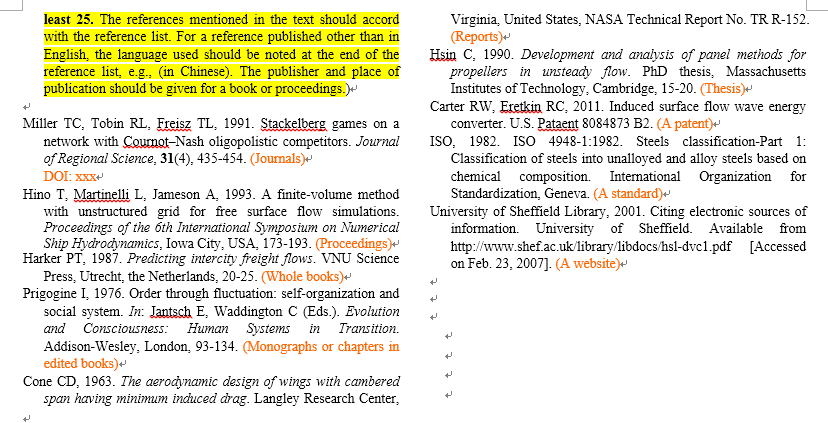
\includegraphics[width=0.9\textwidth]{project-ega-bibliography.png}
  \caption{定制项目文献表示例}\label{fig:proj:bibl:ega}
\end{figure}

\begin{figure}[!htb]
  \centering
  
\includegraphics[width=0.5\textwidth]{project-ega-citation.png}
  \caption{定制项目引用标签示例}\label{fig:proj:cite:ega}
\end{figure}

相比之下,这种只有有限示例,而没有像GB/T7714-2015标准那样详细规定的样式,开发起来会自由一些,因为只要实现示例中的格式即可,未定义的作者可以自己把握,而不需要详细测试每一条规定。此外因为该格式只有英文文献,语言只有英文,也不存在多语言的问题。但该格式也有一些有挑战的东西,特别是引用标签与文献表的作者标签存在明显不同,对于使用相同钩子的两个标签,可能需要特别的处理,以实现不同的格式。

参考文献样式的定制前面已经有了初步介绍,详见\ref{sec:style:def}节,本项目开发也是类似的,关于定制的基本方法不再赘述,下面主要介绍定制需要的所有功能是如何实现的。

\subsubsection{bbx文件开发}
如前所述,biblatex样式文件开发方法,有一个非常便捷的方式是基于标准样式进行。这种方式不仅相对简单,而且对biblatex的兼容性也更好。当biblatex升级时,除非有api改动,绝大多数情况下可以不用修改即可复用。

在本项目开发中,可以看到参考文献表的样式与标准样式很像,因此完全可以在其基础上进行开发,同时还可以利用gb7714-2015ay样式,其中有不少符合中文规范的处理。本项目主要利用这两个样式的代码进行开发。

\paragraph{文献表环境}

看文献表的第一眼可以观察到各条目的缩进格式,即第一行顶格,第二行开始缩进约3个字母宽度,这是由biblatex参考文献环境控制,通常是list环境构建,设置合适的参数就可以实现目标。

\begin{codetex}{重定义参考文献环境确定缩进}{eg:proj:bibenv}
%=====================================================================
%参考文献列表环境
%=====================================================================
  \defbibenvironment{bibliography}%修改参考文献列表环境,不要缩进
  {\list
     {}
     {%\setlength{\leftmargin}{\bibhang}%
      %\setlength{\itemindent}{-\leftmargin}%
      \setlength{\leftmargin}{1.5em}%
      \setlength{\itemindent}{-1.5em}%
      \setlength{\itemsep}{\bibitemsep}%
      \setlength{\parsep}{\bibparsep}}}
  {\endlist}
  {\item}
\end{codetex}

\paragraph{作者域处理}
接着我们看示例中个条目类型相同的部分,主要是作者和页码。这里先处理作者域。显然,作者标签有点像中文风格,姓在前,名的缩写为大小首字母,且没有加点。firstname和givenname之间没有空格,姓的后面也没有标点,姓的首字母大写,其它小写。这种格式与gb7714-2015的风格有点像,可以复用其代码,略作大小写修改,同时使用几个钩子将标点和空格处理完毕。

\begin{codetex}{作者域处理}{eg:proj:author}
\renewrobustcmd*{\bibinitperiod}{}
\renewcommand*{\revsdnamepunct}{\space}
\renewcommand*{\bibnamedelimd}{}
\renewcommand*{\bibnamedelima}{}
\renewcommand*{\bibinitdelim}{}

\renewbibmacro*{author}{%
  \ifboolexpr{
    test \ifuseauthor
    and
    not test {\ifnameundef{author}}
  }
    {\usebibmacro{bbx:dashcheck}
       {%\bibnamedash
       \printnames{author}%
       }%
       {\usebibmacro{bbx:savehash}%
        \printnames{author}%
        \iffieldundef{authortype}
          {\setunit{\addspace}}
          {\setunit{\addcomma\space}}}%
     \iffieldundef{authortype}
       {}
       {\usebibmacro{authorstrg}%
        \setunit{\addspace}}}%
    {\global\undef\bbx@lasthash
     \usebibmacro{labeltitle}%
     \setunit*{\addspace}}%
     \setunit{\addcomma\space}%增加一个逗号
  \usebibmacro{date+extrayear}
  }

%biblatex3.3版后(比如texlive2016中的3.4版)的使用方式
\renewbibmacro*{name:given-family}[4]{%利用family-given定义given-family
  \ifuseprefix
    {\usebibmacro{name:delim}{#3#1}%
     \usebibmacro{name:hook}{#3#1}%
     \ifdefvoid{#3}{}{%
       \ifcapital
         {\mkbibnameprefix{\MakeCapital{#3}}\isdot}
         {\mkbibnameprefix{#3}\isdot}%
       \ifprefchar{}{\bibnamedelimc}}%
     \ifdefvoid{#2}{\mkbibnamefamily{\MakeCapital{#1}}}{\mkbibnamefamily{\MakeSentenceCase{#1}}}\isdot
     \ifdefvoid{#2}{}{\revsdnamepunct\bibnamedelimd\mkbibnamegiven{\MakeUppercase{#2}}\isdot}%\MakeCapital{#2}
     \ifdefvoid{#4}{}{\bibnamedelimd\mkbibnamesuffix{#4}\isdot}}
    {\usebibmacro{name:delim}{#1}%
     \usebibmacro{name:hook}{#1}%
     \ifdefvoid{#2}{\mkbibnamefamily{\MakeCapital{#1}}}{\mkbibnamefamily{\MakeSentenceCase{#1}}}\isdot
     %
     \ifboolexpe{%
       test {\ifdefvoid{#2}}
       and
       test {\ifdefvoid{#3}}}
       {}
       {\revsdnamepunct}%
     \ifdefvoid{#2}{}{\bibnamedelimd\mkbibnamegiven{\MakeUppercase{#2}}\isdot}%\MakeCapital{#2}
     \ifdefvoid{#3}{}{\bibnamedelimd\mkbibnameprefix{#3}\isdot}
     \ifdefvoid{#4}{}{\bibnamedelimd\mkbibnamesuffix{#4}\isdot}}}

\renewbibmacro*{name:family-given}[4]{%利用family-given定义given-family
  \ifuseprefix
    {\usebibmacro{name:delim}{#3#1}%
     \usebibmacro{name:hook}{#3#1}%
     \ifdefvoid{#3}{}{%
       \ifcapital
         {\mkbibnameprefix{\MakeCapital{#3}}\isdot}
         {\mkbibnameprefix{#3}\isdot}%
       \ifprefchar{}{\bibnamedelimc}}%
     \ifdefvoid{#2}{\mkbibnamefamily{\MakeCapital{#1}}}{\mkbibnamefamily{\MakeSentenceCase{#1}}}\isdot
     \ifdefvoid{#2}{}{\revsdnamepunct\bibnamedelimd\mkbibnamegiven{\MakeUppercase{#2}}\isdot}%\MakeCapital{#2}
     \ifdefvoid{#4}{}{\bibnamedelimd\mkbibnamesuffix{#4}\isdot}}
    {\usebibmacro{name:delim}{#1}%
     \usebibmacro{name:hook}{#1}%
     \ifdefvoid{#2}{\mkbibnamefamily{\MakeCapital{#1}}}{\mkbibnamefamily{\MakeSentenceCase{#1}}}\isdot
     %
     \ifboolexpe{%
       test {\ifdefvoid{#2}}
       and
       test {\ifdefvoid{#3}}}
       {}
       {\revsdnamepunct}%
     \ifdefvoid{#2}{}{\bibnamedelimd\mkbibnamegiven{\MakeUppercase{#2}}\isdot}%%\MakeCapital{#2}
     \ifdefvoid{#3}{}{\bibnamedelimd\mkbibnameprefix{#3}\isdot}
     \ifdefvoid{#4}{}{\bibnamedelimd\mkbibnamesuffix{#4}\isdot}}}
\end{codetex}

此外,多个姓名之间用逗号分隔,最后一个姓名前不用and,而使用逗号,可以通过使用钩子以及处理本地化字符串and来实现。
\begin{codetex}{本地化字符串处理}{eg:proj:localbibstr}
\DefineBibliographyStrings{english}{
and         = {\addcomma},%将第2和3人名见的and符号改成 逗号,用\finalnamedelim命令也可以定义,参见3.9.1节
byeditor    = {\mkbibparens{Eds\adddot\isdot}},
urlseen     = {Accessed on},
january          = {Jan\adddot},
february         = {Feb\adddot},
  march            = {Mar\adddot},
  april            = {Apr\adddot},
  may              = {May},
  june             = {June},
  july             = {July},
  august           = {Aug\adddot},
  september        = {Sept\adddot},
  october          = {Oct\adddot},
  november         = {Nov\adddot},
  december         = {Dec\adddot},
}
\end{codetex}

\paragraph{条目类型及其使用的域}

接下来我们首先来看一下示例中所给出的条目类型(表\ref{tab:proj:entrytypes})及其所使用的域。
\begin{table}[!hbtp]
\centering
\caption{支持的条目类型}\label{tab:proj:entrytypes}
\begin{tabular}{|l|c|l|}
  \hline
  % after \\: \hline or \cline{col1-col2} \cline{col3-col4} ...
  entry type  &  & references \\ \hline
article                        & for & journals' paper \\
inproceedings                  & for & proceedings' paper\\
book                           & for & whole books\\
inbook                         & for & monographs or chapters in edited books\\
report                         & for & reports\\
thesis/phdthesis/masterthesis  & for & thesis\\
patent                         & for & patents\\
standard                       & for & standards\\
online/www                     & for & websites  \\
  \hline
\end{tabular}
\end{table}

根据对各条目内容的分析可以得到各条目使用的域为:
\begin{codetex}{各条目使用的域}{eg:proj:fields}
article:
author,date or year.title.journaltitle,volume(number),pages.doi

inproceedings:
author,date or year.title.booktitle.publisher,address or location,pages

book:
author,date or year.title.edition.publisher,address or location,pages

inbook:
author,date or year.title.editor or bookauthor.booktitle.edition.publisher,address or location,pages

report:
author,date or year.title.publisher,address or location.type or number,pages

thesis/phdthesis/masterthesis:
author,date or year.title.type.institution,address or location,pages

patent:
author,date or year.title.number

standard:
author,date or year.title.translator.publisher,address or location,pages

online/www:
author,date or year.title.organization.url.urldate
\end{codetex}

\paragraph{article类型处理}
article条目中,标题为正常字体,期刊名为斜体,卷为粗体,期用圆括号包围,页码前面的符号为逗号,无引导词如pp.,而且doi需要换行。

修改期刊名钩子,卷期定义一个新的域格式,调整页码的引导符,修改doi格式,可以处理完成。
\begin{codetex}{article条目处理}{eg:proj:article}
\DeclareFieldFormat{journaltitle}{\mkbibitalic{#1}\isdot}%添加\isdot,用于缩写名带点情况,将其转换为缩写点便于标点追踪
\DeclareFieldFormat%将期刊等文献的标题中原来带的引号去掉
  [article,patent,unpublished,incollection,inproceedings,inbook]
  {title}{#1\adddot\addthinspace}
\DeclareFieldFormat{titlecase}{\MakeCapital#1}%重设标题格式,将其修改为首字母大写

\DeclareFieldFormat{pages}{#1}%去掉前面引导页码的pp.等字符

\DeclareFieldFormat{addnumflag}{%%增加一个number带括号的格式,避免使用mkbibparens而引入一个不必要的空格
\nobreak\printtext{(}\nobreak #1\nobreak\printtext{)}}
\DeclareFieldFormat{addvolflag}{\mkbibbold{#1}}

\renewbibmacro*{journal+issuetitle}{%
  \usebibmacro{journal}%
  \setunit*{\addspace}%
  \iffieldundef{series}
    {\setunit{\addcomma\addspace}}
    {\newunit
     \printfield{series}%
     \setunit{\addcomma\addspace}}%
  \usebibmacro{volume+number+eid}%
  \setunit{\addcomma\addspace}%
  \usebibmacro{issue+date}%
  \setunit{\addcolon\space}%
  \usebibmacro{issue}%
  \newunit}

\newbibmacro*{journal}{%
  \iffieldundef{journaltitle}
    {}
    {\printtext[journaltitle]{%
       \printfield{journaltitle}%
       \setunit{\subtitlepunct}%
       \printfield{journalsubtitle}}}}

%调整期刊卷和期的格式,
\renewbibmacro*{volume+number+eid}{%
  \printfield[addvolflag]{volume}%
  %\setunit*{\adddot}%去掉点号
  %\printfield{number}%
  \iffieldundef{number}{}{\printfield[addnumflag]{number}}%
  %\iffieldundef{number}{}{\printtext{\mkbibparens{\printfield{number}}}}% 增加一个圆括号
  \iffieldundef{eid}{}{%
  \setunit{\addcomma\space}%
  \printfield{eid}}}

\renewbibmacro*{doi+eprint+url}{%
  \iftoggle{bbx:eprint}
    {\usebibmacro{eprint}}
    {}%
  \newunit\newblock
  \iftoggle{bbx:url}
    {\usebibmacro{url+urldate}}
    {}
  \newunit\newblock
  \iftoggle{bbx:doi}
    {\iffieldundef{doi}{}{\printtext{\newline}}\printfield{doi}}%注意这里printtext的运用,避免前面点的跳行
    {}}

%修改article的驱动,期刊文章,连续出版物中的析出文献的格式
\DeclareBibliographyDriver{article}{%
  \usebibmacro{bibindex}%
  \usebibmacro{begentry}%
  \usebibmacro{author/translator+others}%
  \setunit{\printdelim{nametitledelim}}\newblock
  \usebibmacro{title}%
  \newunit
  \printlist{language}%
  \newunit\newblock
  \usebibmacro{byauthor}%
  \newunit\newblock
  \usebibmacro{bytranslator+others}%
  \newunit\newblock
  \printfield{version}%
  \newunit\newblock
  %\usebibmacro{in:}%
  \usebibmacro{journal+issuetitle}%
  \newunit
  \usebibmacro{byeditor+others}%
  \newunit
  \usebibmacro{note+pages}%
  \newunit\newblock
  \iftoggle{bbx:isbn}
    {\printfield{issn}}
    {}%
  \newunit\newblock
  \usebibmacro{doi+eprint+url}%
  \newunit\newblock
  \usebibmacro{addendum+pubstate}%
  \setunit{\bibpagerefpunct}\newblock
  \usebibmacro{pageref}%
  \newunit\newblock
  \iftoggle{bbx:related}
    {\usebibmacro{related:init}%
     \usebibmacro{related}}
    {}%
  \usebibmacro{finentry}}
\end{codetex}

\paragraph{inproceedings类型处理}

标题为正常字体,文集名为斜体,需要出版项,同时观察book,report类型可以发现,出版项中,出版者在前,出版地在后,中间逗号连接,出版者缺省时不输出。

修改文集名的钩子,修改出版项格式,页码由前面的article中做的全局处理实现。注意到文集名后出版项前的符号是逗号,但这里使用了点号,因为作者认为这样更合理,不同信息块之间通常是由点分隔,示例中绝大部分情况都是如此。当然用逗号分隔也没有任何难度,只需在驱动中出版项前加入一个逗号标点即可。
\begin{codetex}{inproceedings条目处理}{eg:proj:inproceedings}
\DeclareFieldFormat{maintitle}{\mkbibemph{#1}}
\DeclareFieldFormat{booktitle}{\mkbibemph{#1}}
\DeclareFieldFormat%将期刊等文献的标题中原来带的引号去掉
  [article,patent,unpublished,incollection,inproceedings,inbook]
  {title}{#1\adddot\addthinspace}

\renewbibmacro*{publisher+location+date}{%
\printlist{publisher}
\iflistundef{location}{}{\setunit*{\addcomma\space}}%
  \printlist{location}%%
  \setunit*{\addcomma\space}%
  \usebibmacro{date}%
  \newunit}

%会议论文格式修改
\DeclareBibliographyDriver{inproceedings}{%
  \usebibmacro{bibindex}%
  \usebibmacro{begentry}%
  \usebibmacro{author/translator+others}%
  \setunit{\printdelim{nametitledelim}}\newblock
  \usebibmacro{title}%
  \newunit
  \printlist{language}%
  \newunit\newblock
  \usebibmacro{byauthor}%
  \newunit\newblock
  %\usebibmacro{in:}%
  \usebibmacro{maintitle+booktitle}%
  \newunit\newblock
  \usebibmacro{event+venue+date}%
  \newunit\newblock
  \usebibmacro{byeditor+others}%
  \newunit\newblock
  \iffieldundef{maintitle}
    {\printfield{volume}%
     \printfield{part}}
    {}%
  \newunit
  \printfield{volumes}%
  \newunit\newblock
  \usebibmacro{series+number}%
  \newunit\newblock
  \printfield{note}%
  \newunit\newblock
  \printlist{organization}%
  \newunit
  \usebibmacro{publisher+location+date}%
  \newunit\newblock
  \usebibmacro{chapter+pages}%
  \newunit\newblock
  \iftoggle{bbx:isbn}
    {\printfield{isbn}}
    {}%
  \newunit\newblock
  \usebibmacro{doi+eprint+url}%
  \newunit\newblock
  \usebibmacro{addendum+pubstate}%
  \setunit{\bibpagerefpunct}\newblock
  \usebibmacro{pageref}%
  \newunit\newblock
  \iftoggle{bbx:related}
    {\usebibmacro{related:init}%
     \usebibmacro{related}}
    {}%
  \usebibmacro{finentry}}
\end{codetex}

\paragraph{book类型处理}
书名为斜体,出版项使用与inproceedings一致的全局处理。驱动无需修改使用标准样式提供的即可。
\begin{codetex}{book条目处理}{eg:proj:book}
\DeclareFieldFormat%
  [book,report,thesis]
  {title}{\mkbibemph{#1}}
\end{codetex}


\paragraph{inbook类型处理}
章节名正常字体,全书名为斜体,同时全书还需要作者或编者,章节和书名之间用in:表示,出版项和页码使用前述的全局处理。
设置书名钩子,处理in的本地化字符串格式后,最重要是是全书编者中跟着的提示信息(Eds.)。这种提示信息常是由本地化字符串提供,显然eds表示编者,通常全书的作者还可以用bookauthor域表示,但这里为了体现eds信息,使用editor域,于是我们需要对editor域输出格式做修改,得到符合要求的结果。其中byeditor本地化字符串处理,见例\ref{eg:proj:localbibstr}。
\begin{codetex}{inbook条目处理}{eg:proj:inbook}
\DeclareFieldFormat{maintitle}{\mkbibemph{#1}}
\DeclareFieldFormat{booktitle}{\mkbibemph{#1}}

\renewbibmacro*{in:}{%
  \printtext{%
    \mkbibitalic{\bibstring{in}}\intitlepunct}}

\renewbibmacro*{byeditor+others}{%
  \ifnameundef{editor}
    {}
    {\printnames[byeditor]{editor}%
     \setunit{\addspace}%
     \usebibmacro{byeditor+othersstrg}%
     \clearname{editor}%
     \newunit}%
  \usebibmacro{byeditorx}%
  \usebibmacro{bytranslator+others}}

%修改inbook的驱动
\DeclareBibliographyDriver{inbook}{%
  \usebibmacro{bibindex}%
  \usebibmacro{begentry}%
  \usebibmacro{author/translator+others}%
  \setunit{\printdelim{nametitledelim}}\newblock
  \usebibmacro{title}%
  \newunit
  \printlist{language}%
  \newunit\newblock
  \usebibmacro{byauthor}%
  \newunit\newblock
  \usebibmacro{in:}%
  \usebibmacro{bybookauthor}%
  \newunit\newblock
  \usebibmacro{byeditor+others}%
  \newunit\newblock
  \usebibmacro{maintitle+booktitle}%
  \newunit\newblock
  \printfield{edition}%
  \newunit
  \iffieldundef{maintitle}
    {\printfield{volume}%
     \printfield{part}}
    {}%
  \newunit
  \printfield{volumes}%
  \newunit\newblock
  \usebibmacro{series+number}%
  \newunit\newblock
  \printfield{note}%
  \newunit\newblock
  \usebibmacro{publisher+location+date}%
  \newunit\newblock
  \usebibmacro{chapter+pages}%
  \newunit\newblock
  \iftoggle{bbx:isbn}
    {\printfield{isbn}}
    {}%
  \newunit\newblock
  \usebibmacro{doi+eprint+url}%
  \newunit\newblock
  \usebibmacro{addendum+pubstate}%
  \setunit{\bibpagerefpunct}\newblock
  \usebibmacro{pageref}%
  \newunit\newblock
  \iftoggle{bbx:related}
    {\usebibmacro{related:init}%
     \usebibmacro{related}}
    {}%
  \usebibmacro{finentry}}
\end{codetex}

\paragraph{report类型处理}
在report类中,标题为斜体,后面是出版项,和报告类型及编号。修改驱动调整出版项和报告类型的顺序。也要注意两者之间示例给出的逗号分隔符,这里作者仍然使用了点号,原因如前所述,不同信息块的分隔用点号,当然如果要改成逗号也非常简单。唯一需要注意的是,通常报告的出版者用institution域表示,所以对其做域publisher类似的处理。
\begin{codetex}{report条目处理}{eg:proj:report}
\DeclareFieldFormat%
  [book,report,thesis]
  {title}{\mkbibemph{#1}}

\renewbibmacro*{institution+location+date}{%
  \printlist{institution}%
  \iflistundef{location}{}{\setunit*{\addcomma\space}}%
  \printlist{location}%
  \setunit*{\addcomma\space}%
  \usebibmacro{date}%
  \newunit}

%report
\DeclareBibliographyDriver{report}{%
  \usebibmacro{bibindex}%
  \usebibmacro{begentry}%
  \usebibmacro{author}%
  \setunit{\printdelim{nametitledelim}}\newblock
  \usebibmacro{title}%
  \newunit
  \printlist{language}%
  \newunit\newblock
  \usebibmacro{byauthor}%
  \newunit\newblock
  \printfield{version}%
  \newunit
  \printfield{note}%
  \newunit\newblock
  \usebibmacro{institution+location+date}%
  \newunit\newblock
  \printfield{type}%
  \setunit*{\addspace}%
  \printfield{number}%
  \newunit\newblock
  \usebibmacro{chapter+pages}%
  \newunit
  \printfield{pagetotal}%
  \newunit\newblock
  \iftoggle{bbx:isbn}
    {\printfield{isrn}}
    {}%
  \newunit\newblock
  \usebibmacro{doi+eprint+url}%
  \newunit\newblock
  \usebibmacro{addendum+pubstate}%
  \setunit{\bibpagerefpunct}\newblock
  \usebibmacro{pageref}%
  \newunit\newblock
  \iftoggle{bbx:related}
    {\usebibmacro{related:init}%
     \usebibmacro{related}}
    {}%
  \usebibmacro{finentry}}
\end{codetex}

\paragraph{thesis类型处理}
标题是斜体,带论文类型,后面是出版项和页码。标题修改使用钩子,出版项和页码使用前述的全局设置。主要是论文类型。目前没有做任何的额外处理,因为biblatex自动会将phdthesis,masterthesis转换为thesis,并设置type。如果用户直接使用thesis,并且需要type信息,那么需要在type域中输入类型是phdthesis或masterthesis。

\paragraph{patent类型处理}
标题为正常字体,后面跟专利号。无需任何处理。

\paragraph{standard类型处理}
因为standard类型在biblatex中没有定义,因此需要增加一个standard类型的驱动,类似于book的驱动,只是标题改为正常字体。

\begin{codetex}{standard条目处理}{eg:proj:standard}
%增加标准的驱动
\DeclareBibliographyDriver{standard}{%
  \usebibmacro{bibindex}%
  \usebibmacro{begentry}%
  \usebibmacro{author/editor+others/translator+others}%
  \setunit{\printdelim{nametitledelim}}\newblock
  \usebibmacro{maintitle+title}%
  \newunit
  \printlist{language}%
  \newunit\newblock
  \usebibmacro{byauthor}%
  \newunit\newblock
  \usebibmacro{byeditor+others}%
  \newunit\newblock
  \printfield{edition}%
  \newunit
  \iffieldundef{maintitle}
    {\printfield{volume}%
     \printfield{part}}
    {}%
  \newunit
  \printfield{volumes}%
  \newunit\newblock
  \usebibmacro{series+number}%
  \newunit\newblock
  \printfield{note}%
  \newunit\newblock
  \usebibmacro{publisher+location+date}%
  \newunit\newblock
  \usebibmacro{chapter+pages}%
  \newunit
  \printfield{pagetotal}%
  \newunit\newblock
  \iftoggle{bbx:isbn}
    {\printfield{isbn}}
    {}%
  \newunit\newblock
  \usebibmacro{doi+eprint+url}%
  \newunit\newblock
  \usebibmacro{addendum+pubstate}%
  \setunit{\bibpagerefpunct}\newblock
  \usebibmacro{pageref}%
  \newunit\newblock
  \iftoggle{bbx:related}
    {\usebibmacro{related:init}%
     \usebibmacro{related}}
    {}%
  \usebibmacro{finentry}}
\end{codetex}

\paragraph{online类型处理}
最后是online类型,标题后跟的是组织,后面跟的是网址及其访问日期。主要要修改的是url和urldate的域格式。因为urldate域需要提供所有的年月日信息,所以设置urldate宏包选项,注意区别于date域的选项。同时因为其特殊的形式,修改月份的本地化字符串,如例\ref{eg:proj:localbibstr}所示。

\begin{codetex}{online条目处理}{eg:proj:online}
\ExecuteBibliographyOptions{
  useprefix = true,  %名字的信息包括前缀
  %firstinits = true,    %名字有缩写,参考3.1.2.3 Internal
  giveninits = true,
  date   = year,  %日期仅写到年
  urldate= comp,
  %maxnames     = 3 , %设置名字最大数量
  %minnames     = 3,  %设置缩减后的名字最小数量
  maxbibnames=3, %将文献列表和引用中最大名字数量区分开
  minbibnames=3,
}

\DeclareFieldFormat{url}{Available from\space\url{#1}}
\DeclareFieldFormat{urldate}{\mkbibbrackets{\bibstring{urlseen}\space#1}}
\end{codetex}

\paragraph{全局选项及texlive兼容性处理}
全局选项设置如例\ref{eg:proj:online}所示,使用类似于gb7714-2015的设置,使用姓名前缀和缩写,设置文献表中作者标签最大和最小姓名数为3。

对于biblatex的兼容性,因为升级可能带来的变化,这里特别做了处理,主要是texlive2016和texlive2017,其中的biblatex版本分别为3.4和3.7。对于本项目,其中有一个命令存在差异,因此换个版本会报错,因此特别做出处理,处理方式类似于gb7714-2015样式。

\begin{codetex}{texlive兼容性处理}{eg:proj:texlive}
\providetoggle{iftexlivesix}
\providetoggle{iftexliveseven}%为处理texlive2016到2017的变化
%版本判断,根据biblatex更新历史可知,版本3.3开始使用新的姓名机制
%所以当版本大于3.2开始,就用设置\toggletrue{iftexlivesix}
\def\numparserta#1.#2\relax{#1}%注意relax的重要性
\def\numparsertb#1.#2\relax{#2}
\def\numinteger{\expandafter\numparserta\abx@version\relax}
\def\numdigital{\expandafter\numparsertb\abx@version\relax}
\ifnumcomp{\numdigital}{>}{2}{\toggletrue{iftexlivesix}}{\togglefalse{iftexlivesix}}
\ifnumcomp{\numdigital}{>}{6}{\toggletrue{iftexliveseven}}{\togglefalse{iftexliveseven}}

\iftoggle{iftexliveseven}{%
  \renewbibmacro*{date+extrayear}{%
    \iffieldundef{labelyear}
      {}
      {\printtext{%[parens]%这里把括号去掉
         \iffieldsequal{year}{labelyear}
           {\printlabeldateextra}%
           {\printfield{labelyear}%
            \printfield{extrayear}}}}}%
}{%
\renewbibmacro*{date+extrayear}{%
    \iffieldundef{\thefield{datelabelsource}year}
      {}
      {\printtext{%[parens]%这里把括号去掉
         \iffieldsequal{year}{\thefield{datelabelsource}year}
           {\printdateextralabel}%
           {\printfield{labelyear}%
            \printfield{extrayear}}}}}%
}
\end{codetex}

如此完成了bbx文件的开发。

\subsubsection{cbx文件开发}
下面进行cbx文件开发。cbx引用标签样式示例给出了3个。分别是1位作者、2位、3位或以上作者的情况。可以看到2位作者时全部给出,超过3位则只给出一位,这可以通过设置宏包选项实现,例\ref{eg:proj:cbxopt}中给出的其它选项,与gb7714-2015相同。单个姓名的标签采用默认的方式处理,作者和年份之间的分隔符,修改对应的钩子即可。

\begin{codetex}{cbx设置宏包选项}{eg:proj:cbxopt}
\ExecuteBibliographyOptions{
  %autocite  = superscript ,
  %autopunct = true       ,
  %sorting   = none        ,
  maxcitenames=2,
  mincitenames=1,
  uniquename=init,%因为使用了名字缩写选项,所以需要设置uniquename=init而不是full避免冲突
  labeldate=true,
  uniquelist=minyear,
}

\DeclareDelimFormat{nameyeardelim}{\addcomma\addspace}
\end{codetex}

除此之外,还有几个格式需要实现,包括:
\begin{itemize}
  \item et al. 的斜体
  \item 两位作者时,and连接
  \item 同作者文献,连续出现,作者名只出现一次
\end{itemize}

这三个问题其实是本项目最复杂的地方。因为一般情况下,引用标签与文献表中的作者标签使用相同的钩子,因此格式相同。那么在文献表中作者格式确定的情况下,无法全局的重定义这些钩子,否则会影响文献表。

好在tex的作用域机制保证了重定义可以作用在局部范围内。于是重定义name:andothers宏来实现etal斜体,重定义finalnamedelim来实现and连接。但是作者省略的问题,还无法解决,思考解决方法,找到authoryear文献表中存在的省略,这里其实也可以复用其中的宏,于是新定义一个cite:labelname取代直接打印姓名的方式,重定义cite宏实现要求,最后重定义cite命令,在引用标签外加上圆括号。

\begin{codetex}{cbx重定义实现要求}{eg:proj:cbxredef}
\newbibmacro*{cite:labelname}{%
    \usebibmacro{bbx:dashcheck}%
       {}%\bibnamedash%
       {\usebibmacro{bbx:savehash}%
        \printnames{labelname}%
        \setunit{\printdelim{nameyeardelim}}}}

\renewbibmacro*{cite}{%
  \iffieldundef{shorthand}%
    {\ifthenelse{\ifnameundef{labelname}\OR\iffieldundef{labelyear}}%
       {\usebibmacro{cite:label}%
        \setunit{\printdelim{nonameyeardelim}}}%
       {\renewcommand*{\finalnamedelim}{%
  \ifnumgreater{\value{liststop}}{2}{\finalandcomma}{}%
  \addspace and\space}%
  \renewbibmacro*{name:andothers}{%
  \ifboolexpr{%
    test {\ifnumequal{\value{listcount}}{\value{liststop}}}
    and
    test \ifmorenames
  }%
    {\ifnumgreater{\value{liststop}}{1}%
       {\finalandcomma}%
       {}%
     \andothersdelim\mkbibemph{\bibstring{andothers}}}%
    {}}%
\usebibmacro{cite:labelname}%\printnames{labelname}%
}%
\usebibmacro{cite:labelyear+extrayear}}%
    {\usebibmacro{cite:shorthand}}}

%\DeclareCiteCommand{\cite}[\mkbibparens]{⟨precode⟩}{⟨loopcode⟩}{⟨sepcode⟩}{⟨postcode⟩}
%
\DeclareCiteCommand{\cite}[\mkbibparens]
  {\usebibmacro{prenote}}
  {\usebibmacro{citeindex}%
   \usebibmacro{cite}}
  {\multicitedelim}
  {\usebibmacro{postnote}}
\end{codetex}

到此,我们完成了所有的开发。

项目所有文档见:
\href{run:./exampleandimage/egzazhi.tex}{egzazhi.tex},
\href{run:./exampleandimage/zazhi.bbx}{zazhi.bbx},
\href{run:./exampleandimage/zazhi.cbx}{zazhi.cbx},
\href{run:./exampleandimage/egbib.bib}{egbib.bib}。

结果如图\ref{fig:proj:res}所示。

\begin{figure}[!htb]
  \centering
  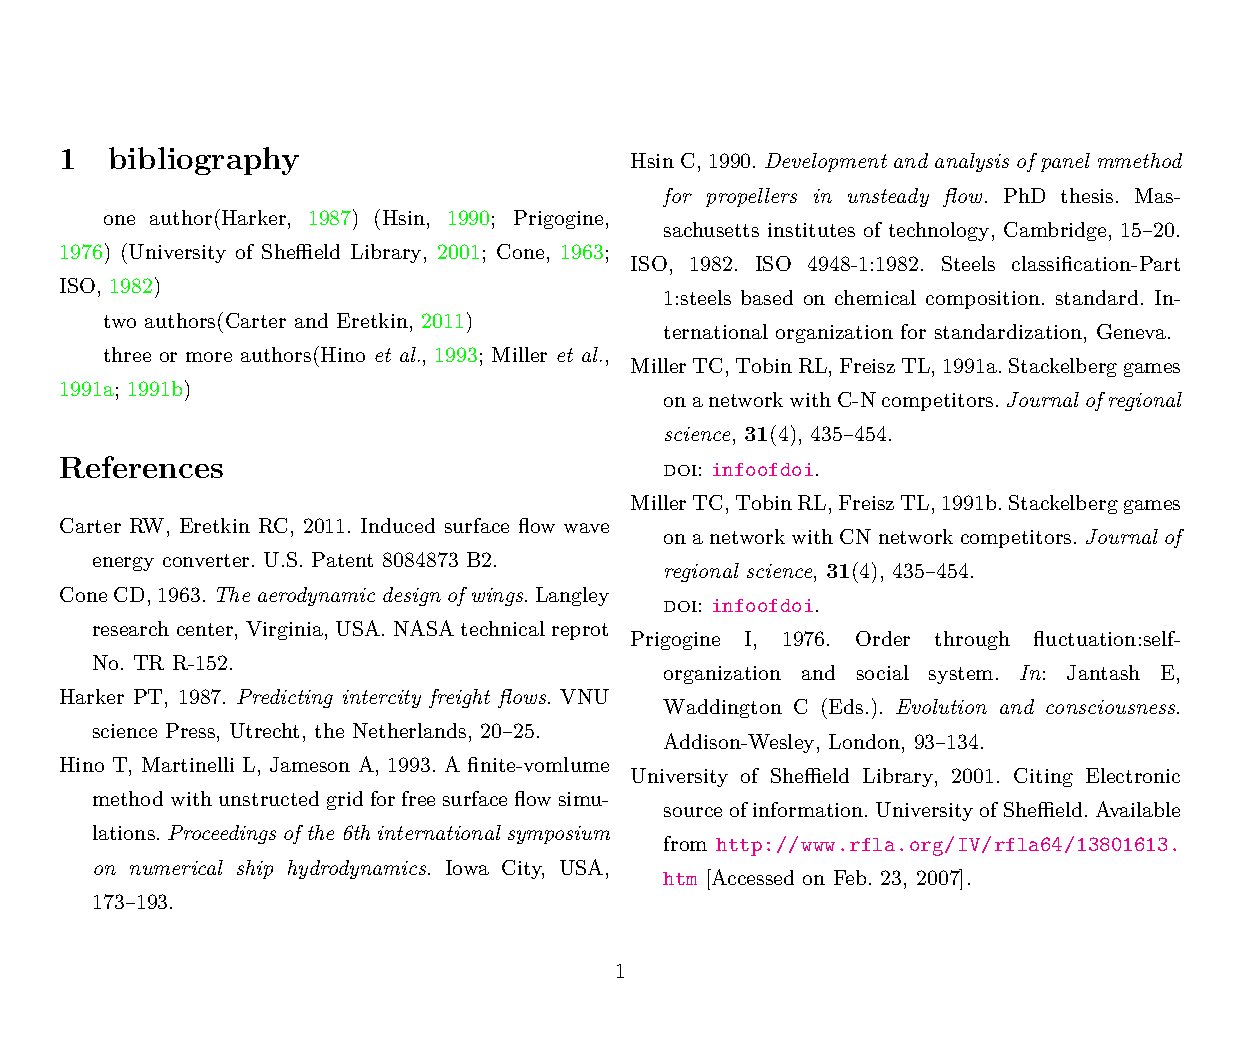
\includegraphics[width=0.9\textwidth,page=1]{egzazhi.pdf}
  \caption{样式定制结果}\label{fig:proj:res}
\end{figure}


\subsubsection{小结}
通过上述实践,我们完成了一个定制项目,可以看到biblatex的强大,它提供的api相当全面和有效,利用它以及标准样式可以较为方便构建满足需要的定制格式。

\section{结论}
通过本文的工作给出了\LaTeX 文档中文参考文献相关问题的biblatex解决方案,包括: 基本参考文献生成、分章参考文献、指定格式的著录和标注样式等,基本能够满足日常的各类参考文献生成需求,能够为\LaTeX 文档写作提供帮助。

\section{后记}
因水平有限,难免存在一些错误,请各位朋友批评指正。如果遇到什么问题,也可以邮件联系,欢迎交流。

%%----------------------------------------------------------------
\printbibliography[heading=subbibliography,title=参考文献]
%\end{multicols}
\end{refsection}
\clearpage 
%%一篇论文结束
%%----------------------------------------------------------------


%%================================================================
%%下一篇论文,格式与上一篇类似,只要修改内容即可
%%----------------------------------------------------------------
%新的一篇论文放到articlesecond.tex文件中,后面的新论文类似,通常不包含进来。


%为方便超链接查看,这里可以加入目录
\vspace{1cm}
\noindent\rule{\linewidth}{3pt}
\phantomsection
\addcontentsline{toc}{section}{目录}
\tableofcontents
%\renewcommand{\numberline}[1]{#1~}
\phantomsection
\addcontentsline{toc}{section}{插图}
\listoffigures
\phantomsection
\addcontentsline{toc}{section}{表格}
\listoftables
\phantomsection
\addcontentsline{toc}{section}{示例}
\listofegcode



\end{document} 